%TEX-template borrowed from https://github.com/idlouhy/wonsole/blob/master/report/src/report.tex

\documentclass[10pt,b5paper,twoside,openright]{report}

\usepackage[section] {placeins}

\usepackage{changepage}

\raggedbottom

\usepackage[english]{babel}
\usepackage[utf8]{inputenc}
\usepackage[T1]{fontenc}
\usepackage{float}

\selectlanguage{english}

\usepackage[usenames,dvipsnames,svgnames,table]{xcolor}

\usepackage{graphicx}
\usepackage{tabu}
\usepackage{booktabs}
\usepackage{wrapfig}
\usepackage{pbox}
\usepackage{pgfplots}
\usepackage{pgfplotstable}
\usepackage{longtable}
\usepackage{pdfpages}
\usepackage{emptypage}

\usepackage{nameref}
\usepackage{fullpage}
\usepackage{verbatim}
\usepackage{url}
\usepackage{minitoc}
\usepackage{cite}
\usepackage{caption}
\usepackage{float}
\usepackage{color}
\usepackage{pgfgantt}
\usepackage{listings}
%\usepackage{xcolor}
\usepackage{multirow}

%\usepackage{mdframed}
\usepackage[most]{tcolorbox}

\usepgfplotslibrary{dateplot}

\usepackage{tikz}
\usetikzlibrary{backgrounds}
\makeatletter

\usepackage{pdflscape}

\usepackage{afterpage}

\newcommand\blankpage{%
    \null
    \thispagestyle{empty}%
    \addtocounter{page}{-1}%
    \newpage}

\tikzset{%
  fancy quotes/.style={
    text width=\fq@width pt,
    align=justify,
    inner sep=2.5em,
    anchor=north west,
    minimum width=\textwidth,
  },
  fancy quotes width/.initial={.7\textwidth},
  fancy quotes marks/.style={
    scale=8,
    text=white,
    inner sep=0pt,
  },
  fancy quotes opening/.style={
    fancy quotes marks,
  },
  fancy quotes closing/.style={
    fancy quotes marks,
  },
  fancy quotes background/.style={
    show background rectangle,
    inner frame xsep=0pt,
    background rectangle/.style={
      fill=gray!25,
      rounded corners,
    },
  }
}

\newenvironment{fancyquotes}[1][]{%
\noindent
\tikzpicture[fancy quotes background]
\node[fancy quotes opening,anchor=north west] (fq@ul) at (0,0) {``};
\tikz@scan@one@point\pgfutil@firstofone(fq@ul.east)
\pgfmathsetmacro{\fq@width}{\textwidth - 2*\pgf@x}
\node[fancy quotes,#1] (fq@txt) at (fq@ul.north west) \bgroup}
{\egroup;
\node[overlay,fancy quotes closing,anchor=east] at (fq@txt.south east) {''};
\endtikzpicture}

\makeatother

\setlength{\parindent}{0.0in}
\setlength{\parskip}{1.5ex}

\setlength{\fboxsep}{0pt}
\setlength{\fboxrule}{1pt}

\fontfamily{ptm}\selectfont

\usepackage{hyperref}
\hypersetup{
    bookmarks=true,
    unicode=true,
    pdftoolbar=true,
    pdfmenubar=true,
    pdffitwindow=false,
    pdfstartview={FitH},
    pdftitle={Research Project},
    pdfauthor={Espen Andreassen},
    pdfsubject={Research Project Report},
    pdfkeywords={ntnu} {research project}{large-scale}{agile}{},
    pdfnewwindow=true,
    colorlinks=false,
    linkcolor=blue,
    citecolor=blue,
    filecolor=blue,
    urlcolor=blue
}

\bibliographystyle{ieeetr}
%\bibliographystyle{apalike}

\begin{document}

%TITLE

%\thispagestyle{empty}
%
%\begin{center}
%    {\Huge\textbf{TDT4900 - Computer Science, Master's Thesis}} \\
%    \medskip
%
%\vspace{0.5cm}
%
%    {\huge Coordination Effectiveness in Large-scale Agile Software Development}
%
%    \vspace{6cm}
%
%    {\large Spring 2015}\\
%
%    \vspace{0.5cm}
%
%    {\Large Author:}\\
%    {\large
%    Espen Andreassen\\
%    }
%
%    \vspace{0.5cm}
%
%    {\large
%    Advisor:\\
%    Torgeir Dingsøyr\\}
%
%    \vspace{6cm}
%
%    
\includegraphics[trim = 2mm 0mm 0mm 0mm, width=2.5in]{images/logo-ntnu.pdf}
%
%    
\includegraphics[trim = 0mm 0mm 16mm 0mm, width=3.5in]{images/idi.pdf}
%    \large{Department of\\Computer and Information Science}
%
%\end{center}

%\newpage

\cleardoublepage
\begin{abstract}

In later years agile development methodologies have seen a steady growth. Agile approaches were originally developed for small-scale contexts to cover the increasing need for flexibility and the urge to be first-to-market with technology in constant change. The benefits witnessed in this small-scale adoption has got large organisations to open their eyes. Therefore, it has not been surprising to see large-scale software development projects opt for the use of agile methodologies. However, the research regarding agile development in a large-scale context is still scarce.

Another aspect that has seen an increasing focus in the later years has been coordination effectiveness, which is identified as an important factor in software development and team performance.

These two aspects are combined and looked further into in this research study. The focus is on robust empirical studies performed on coordination in large-scale agile software development projects. Strode's theoretical model of coordination is also looked further into to identify its applicability in a large-scale context.

The main findings show similarities to coordination effectiveness in small-scale agile software development, but also some dissimilarities. Synchronisation, team co-location, an organisational openness culture, and appropriate infrastructure and supportive tools seem to have a positive effect on the team performance. On the other hand, number of sites and team size, as well as large time zone differences between teams, seem to have a negative effect on the level of effectiveness achieved through coordination in large-scale agile software development projects.

\textbf{Keywords:} Large-scale; Coordination; Coordination Effectiveness; Agile Software Development; Scrum

\end{abstract}
\cleardoublepage
\begin{abstract}

In later years agile development methodologies have seen a steady growth. Agile approaches were originally developed for small-scale contexts to cover the increasing need for flexibility and the urge to be first-to-market with technology in constant change. The benefits witnessed in this small-scale adoption has got large organisations to open their eyes. Therefore, it has not been surprising to see large-scale software development projects opt for the use of agile methodologies. However, the research regarding agile development in a large-scale context is still scarce.

Another aspect that has seen an increasing focus in the later years has been coordination effectiveness, which is identified as an important factor in software development and team performance.

These two aspects are combined and looked further into in this research study. The focus is on robust empirical studies performed on coordination in large-scale agile software development projects. Strode's theoretical model of coordination is also looked further into to identify its applicability in a large-scale context.

The main findings show similarities to coordination effectiveness in small-scale agile software development, but also some dissimilarities. Synchronisation, team co-location, an organisational openness culture, and appropriate infrastructure and supportive tools seem to have a positive effect on the team performance. On the other hand, number of sites and team size, as well as large time zone differences between teams, seem to have a negative effect on the level of effectiveness achieved through coordination in large-scale agile software development projects.

\textbf{Keywords:} Large-scale; Coordination; Coordination Effectiveness; Agile Software Development; Scrum

\end{abstract}
\cleardoublepage
\pagenumbering{gobble}
\chapter*{Preface}

I am now fulfilling my last year on a master degree in computer science where I specialise in software, or more specifically, software systems. I was introduced to agile development methodologies through different subjects at the ``Norwegian University of Science and Technology'', NTNU, and also got hands-on experience working with Scrum in a subject called ``TDT4290 - Customer Driven Project''. This subject in particular sparked my interest in agile development methodologies and the new ways of handling work and project organisation. After a summer internship with EY (formerly known as Ernst\&Young) I got more intrigued with how communication and coordination was handled in real life business and IT projects. Therefore, my previous experiences led to a motivation in exploring the combination of agile development and coordination.

The work performed in this master thesis is carried out to give an insight in the field of coordination in large-scale agile software development projects. I hope that the research performed will be beneficial for other research as the topic at hand is still scarcely studied.

I would like to use this opportunity to thank Torgeir Dingsøyr for his support, assistance and knowledge throughout the research project as the supervisor. I would also like to thank NTNU for giving me the opportunity to experiment with ideas within the boundaries of the research project, and letting me acquire interesting knowledge for the future.

\vspace{1.5cm}

Trondheim, \today

\newcommand{\singleSignature}[1]{
\vspace{0.5cm}


\noindent
%\begin{}


    \vspace{0.5cm}

    \begin{tabular}{l}
    \rule{6cm}{1pt}\\
    #1
    \end{tabular}
%\end{}

\vspace{1cm}
}

\singleSignature{Espen Andreassen}

\setcounter{tocdepth}{1}
\dominitoc
\dominilof
\dominilot
\tableofcontents
\clearpage
\listoffigures
\listoftables

% CHAPTERS

\part{Introduction and Theory}
\chapter{Introduction}

\pagenumbering{arabic}

\minitoc

The introduction chapter takes a closer look at the motivation behind the study. It also looks at the concrete problem description and the background for this description, as well as the research question. Afterwards, a closer look at the scope and limitations of the research project is performed. Ending the chapter is a section giving a closer look at the report outline.

\newpage

\section{Motivation}

In 2007 an article on the future of socio-technical coordination in global software engineering was published by James D. Herbsleb \cite{Herbsleb2007}. In this work he gathered previous research carried out on the area of coordination and looked at where future studies could focus their attention. It is interesting to notice that already at such an early stage focus on coordination and effective coordination mechanisms in global projects were present. In his research he highlighted that there was a pressing need for deeper understanding of which kind of coordination that will be required in the globalisation witnessed, and which effect this will have on the business world. This article was one of the main motivators for the master thesis.

Organisations and companies around the world are in a transformation phase with a lot of them transitioning from traditional development methodologies to agile approaches. An example is SAP AG moving from a waterfall-like approach to the introduction of Scrum and a lean development style in a large-scale context. From this transition experiences were extracted. A lot of these experiences focused on the complexity of managing multi-team development when scaling Scrum \cite{Nord2011}. This highlights and motivates the need for focus to be directed towards coordination, collaboration and communication studies in such large-scale agile software development.

As will also be seen in this master thesis the large-scale agile development world is not only present globally, but has slowly taken place at a domestic domain as well. This further shows the topical and relevant nature of the study. The master thesis was in that sense made even more interesting for the researcher because of the case company and project taking place in Norway.

\section{Problem Description and Background}
\label{pdab}

Since the introduction of agile development methodologies their usage have seen a steady growth. This has led to an increasing need for studies that reflect on the consequences and different aspects following the paradigm shift. One of these aspects is how coordination is handled \cite{Agerfalk2006, Leffingwell2007, Cockburn2002, Batra2010}. At the International Conference on Agile Software Development (XP2013) ``Inter-team coordination'' was voted the number one burning topic in large-scale agile software development, with ``Large project organization'' coming in second \cite{Dingsoyr2013b}.  In the latest years there has evidentially been an increase in companies and organisations performing development through agile development methodologies in large-scale projects \cite{Paasivaara2012, Com2013, Vlietland2015, Lindvall2004, Dingsoyr2013b, Lee2008, Paasivaara2009}, but the effects have not been well-documented \cite{Pikkarainen2008, Paasivaara2012, Freudenberg2010, Haaster2014, Dingsoyr2013a, Reifer2003}. In the study this topic will be highlighted with the focus on coordination in large-scale agile projects. Theory, literature and models from the Software-field will be used and compared to other fields to see which changes and similarities the paradigm shift has brought forth (theories and literature from large-scale will be used where this is available).

\begin{fancyquotes}
Which similarities and dissimilarities in inter-team coordination can be found between current literature on large-scale/MTS projects, and a large-scale agile software development project in practice?
\end{fancyquotes}

The purpose of the study and the planned master thesis will therefore be a combination of ``To add to the body of knowledge'', ``To solve a problem'', ``To find the evidence to inform practice'', ''To develop a greater understanding of people and their world'' and ``To contribute to other people's well-being'' \cite{Oates2006}.

While research in small-scale agile software development is starting to get a good track record \cite{Paasivaara2012, Haaster2014}, there is a clear gap in the research surrounding coordination in large-scale agile software development \cite{Pikkarainen2008, Paasivaara2012, Dingsoyr2013b}, and large-scale agile software development in general \cite{Freudenberg2010, Haaster2014}. Therefore, this master thesis will contribute in filling parts of the gap. This will involve ``An exploration of a topic, area or field'', as well as ``An in-depth study of a particular situation'' in the case study \cite{Oates2006}.

As stated above, small-scale agile software development research is starting to get a good track record with successful findings. Because of these findings large organisations have been interested in adopting the benefits agile software development has shown over traditional development methods \cite{Com2013, Vlietland2015, Agerfalk2006, Paasivaara2012}. The assumption that agile methodologies will deliver the same benefits when scaled to larger organisations and projects is therefore an interesting topic.

The combination of filling the gap and looking at the aforementioned assumption will be the pillars in the research outcomes.

\section{Scope, Limitations and Acknowledgement}

As time constraints were put on the master thesis it was obvious that some attention had to be aimed towards the scope of the report and the limitations this would imply. As mentioned in the previous section \ref{pdab} large-scale agile projects, and agile projects in general, are growing in numbers. With this growth a lot of questions and interesting research problems arise. It is therefore important to specify that this particular master thesis only aims to cover the described research question: ``Which similarities and dissimilarities in inter-team coordination can be found between current literature on large-scale/MTS projects, and a large-scale agile software development project in practice?''.

Further, the research project does not aspire to introduce a brand new theory regarding the combination of large-scale, agile software development, coordination and effectiveness. The objective is to find and categorise research performed concerning the combination of these themes and look for common conclusions in their findings, as well as identifying and calling attention to clear gaps that need to be filled in the research field. After this empirical review has been conducted the findings will be compared to a real life case project carried out at a large-scale agile software development project in Norway.

To give some insight and a clearer picture of the study, theory from agile software development, coordination and large-scale will be presented. Findings from a literature review will also be given on the combination of the aforementioned themes. It is important to note that the focus on coordination will primarily be on coordination across teams and not on coordination within these teams.

It is important to acknowledge that some of the work gathered and used in this master thesis was carried out in a preliminary study by the researcher. Some of this work is included in different chapters, e.g., the theory chapter. Also some of this work has been rewritten or made more thorough and elaborated.

Lastly, the research study will not focus on frameworks and electronic tools suggested to support the large-scale agile processes. In this study the focus will rather be aimed towards robust empirical studies performed on the research area of coordination in a large-scale context, as well as the interviews performed with all involved organisations of the Omega-project.

\section{Target Audience}

It is important to have an audience in mind when researching and publishing a work. In this particular master thesis the main effort has been on three types of audiences:

\begin{itemize}
   \item \textbf{Researchers} from the coordination and agile field could find such a research interesting because of the small pool of research articles available on similar work.
   \item \textbf{Practitioners} working with or adopting agile methodologies in a large-scale context might find such a study interesting because it could give insight to possible pitfalls and benefits.
   \item \textbf{Computer science students} could possible find such a work interesting because most of the textbooks and research in general on agile software methodologies and development has only included small-scale projects. It could also give insight to how work is performed in real life projects, and not only how the textbooks describe it.
\end{itemize}

%Researchers, practitioners, fellow computer science students

\section{Report Outline}

\begin{description}
    \item[Chapter 1: Introduction] contains a brief and general introduction to the study at hand and the motivation behind it.
    \item[Chapter 2: Theory] looks at important aspects of the research question, namely software development methodologies, coordination, large-scale, and performance in coordination.
    \item[Chapter 3: Method] explains how the literature review was carried out throughout the research project.
    \item[Chapter 4: Results] outlines the studies selected from the literature review, as well as their findings. It also links these studies to Strode's theoretical model of coordination.
    \item[Chapter 5: Discussion] contains a summarised look at the findings from the results chapter, and connects these to the research question. Strode's theoretical model of coordination is also discussed further with regards to its applicability in a large-scale context.
    \item[Chapter 6: Conclusion] carries out a summary of the most paramount points of the results and discussion chapters.
    \item[Chapter 7: Future Work] outlines possible routes to take in the research field on inter-team coordination.
\end{description}
\chapter{Theory}
\label{theory}

\minitoc

In this chapter theory and literature relevant to the study is presented. It starts of with an introduction of both traditional and agile software development methodologies, with the main focus on Scrum. Afterwards a shift towards coordination is taken. Some well-known literature is looked at, for example Malone and Crowston's coordination theory. Further, to put the study into context, a definition of large-scale is given. To end the chapter a look at different aspects of effectiveness in team coordination is introduced.

\newpage

\section{Software Development Methodologies}

The term software development methodologies has been around for quite some time now. These methodologies are frameworks for accomplishing a well-structured development process. In this section a brief introduction to the most prominent methodologies will be carried out. It will start with a quick look at the traditional software development, before ending with a presentation of the new and agile way of thinking. In the last section (on agile software development) the main focus will be on Scrum as this is the methodology found in most of the literature gathered from the literature review.

\subsection{Traditional Software Development}

Traditional software development methodologies have a distinct pattern. This pattern is sometimes called software development life cycle (SDLC) methodologies which is often found in system engineering. These ``life cycles'' are in contrast to the ``iteration''-approach found in agile methodologies, such as Scrum. The most well-known of these traditional software development methodologies is Waterfall discussed further below.

\subsubsection{Waterfall}

The Waterfall methodology is one of the classic development models. It was first described in a paper by W. W. Royce in 1970 \cite{waterfall}.  The model was not yet named in this paper, which it received later mostly due to its iconic structure (as shown in figure \ref{waterfall}).

In the aforementioned paper, it is suggested that all software development models tend to go through two distinct phases: Analysis and Coding. The author argues that it is not possible to write a software project without having a somewhat deep understanding of the underlying problems that it needs to solve. Therefore an analysis phase will always be required in advance of writing the program itself. However, he also mentions that such a simple model is only suitable for programs that are completed in a matter of days. Larger software projects require an extended number of steps.

For larger projects, the following steps are suggested:
\begin{enumerate}
	\item \textbf{System and Software Requirements:} The customer is involved with the specification of the scope and requirements of the system. The resulting documentation serves as a foundation to the next stages of development.
	\item \textbf{Analysis and Program Design:} The requirements produced in the previous stage are used to create a system plan and various design documents.
	\item \textbf{Coding and Testing:} The actual implementation of the project. This also involves continuously testing on various levels (for example unit and integration).
	\item \textbf{Operation and Maintenance:} Once the project has been completed, it has to be maintained during its usage. In addition to improving the program in various ways, this may also involve the inclusion of extra features if the customer so desires. These features can in themselves use the Waterfall model.
\end{enumerate}

\begin{figure}
\centering
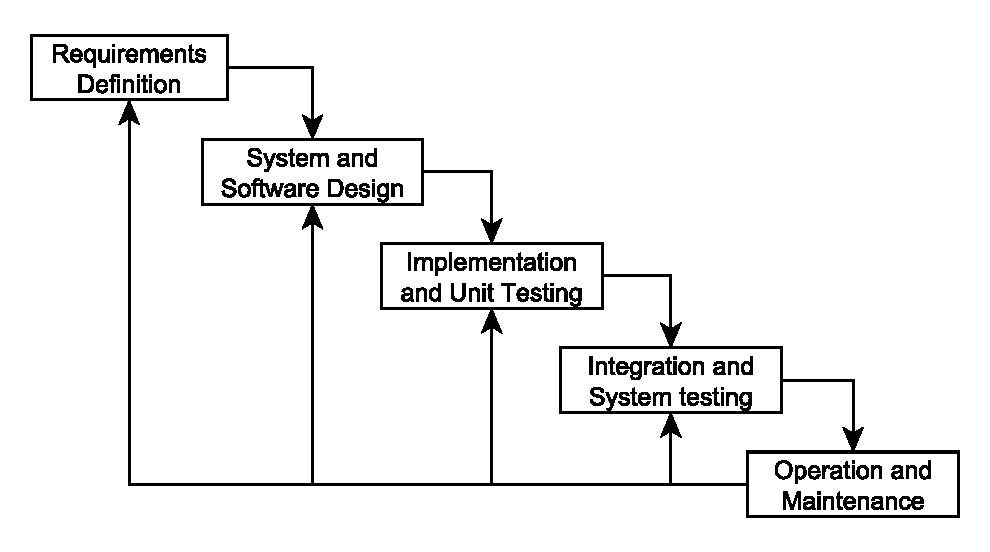
\includegraphics[width=150mm]{images/chapters/development_models/waterfall.pdf}
\caption{The Waterfall model.}
\label{waterfall}
\end{figure}

The model initially suggested by W. W. Royce discusses a linear model in which each of the aforementioned stages are used as distinct steps in the development process. Each stage is required to be completed before the next is started. This may be a sound premise in theory, but as suggested in the paper it is likely to fail in practice. The argument used is that often during development, unforeseen problems in the design are encountered. The linear model does not allow for a return to a previous stage in development. Hence, it does not allow for changes in the design that could potentially resolve such problems.

Therefore, an alternative model is suggested that allows for the process to return to earlier stages if necessary. This may not be an ideal solution either, but it does allow for encountered problems to be addressed during development.

\subsection{Agile Software Development}

As can be seen from the ending of the Waterfall-section there were doubts about its applicability already at an early stage. With the advancement of business needs and customer involvement something had to change. This opened the door for the introduction of a new software development methodology, namely agile software development. This new way of thinking tries to deal with collaboration in a way that promotes adaptive planning, early delivery and continuous improvement, making the development phase faster and more flexible regarding changes \cite{abrahamsson2002}.

\subsubsection{Scrum}
\label{scrum}

In this section an introduction to one of the most popular agile software development methodologies will be carried out, namely Scrum. This is based mainly on Abrahamsson, Salo, Ronkainen and Warsta's publication on agile methods \cite{abrahamsson2002}. In VersionOne's ``7th Annual State of Agile Development Survey'' Scrum or Scrum variants had a quoted 72\% usage making it by far the most popular agile methodology in the survey \cite{Com2013}.

Scrum is an iterative and incremental software development model (as shown in figure \ref{scrum}). It has come forth from the realisation that development methods that were common at the time of its introduction worked well in theory but did not in practice. These methods, Waterfall included, were designed to provide a structured and well-defined development process \cite{scrum}.

The agile software development processes, like Scrum, are part of a recent approach to software development. The idea with Scrum in particular is to divide the development into short periods called ``sprints''. This is done to focus effort for a limited time on short-term goals. Iterating over these goals allows the process to adapt the development plan based on progress but also to address any design problems that arise.

In short, the team concentrates on isolated parts, and through this prioritises on the most important tasks of the project first. The time span of a sprint is typically between one and four weeks long.

In order to implement the requirements step by step and in an orderly fashion, a repository is kept containing the features that have yet to be implemented. This repository is called the ``product backlog''. During development, the requirements could change over time. Therefore the product backlog is not static; it changes to the needs of the project with new topics being added, and obsolete ones being removed. The items from the backlog that a team works on during a sprint is called the ``sprint backlog''.

Meetings are also a key part of Scrum. There are several different types of meetings: sprint planning meeting, daily scrum meeting, backlog refinement, end of cycle and Scrum-of-Scrums. The sprint planning meeting is held at the beginning of each sprint cycle. Here the focus is on what work is to be done, and the sprint backlog for the coming sprint cycle is set. The daily scrum meeting, also called the daily stand-up, is a daily encounter (15 minutes) where each member of the project team answer these three questions:

\begin{enumerate}
  \item What have you done since yesterday?
  \item What are you planning to do today?
  \item Are there any impediments in your way?
\end{enumerate}

Further, there is the backlog refinement, also called ``grooming''. This is where tasks are created, large tasks are decomposed into smaller ones, tasks are prioritised, and the existing tasks are sized in the product backlog. Backlog refinement is often split into two meetings. In the first meeting the product owner and other stakeholders create and refine stories in the backlog. In the second meeting the project team sizes the tasks in the backlog to make them ready for the next sprint. Planning poker is an example of how this can be carried out.

The last listed meeting occurs at the end of each cycle, and is therefore called end of cycle (meeting). This is actually two meetings: a sprint review meeting and a sprint retrospective. At the sprint review meeting the work that is completed and yet to be finished is reviewed. The completed work is also presented for the stakeholders, often called  ``the demo''. At the sprint retrospective all members reflect on the past sprint. Two main questions are answered:

\begin{enumerate}
  \item What went well during the sprint?
  \item What could be improved in the next sprint?
\end{enumerate}

The Scrum team usually consists of five to nine members. It is important to note that Scrum teams do not use traditional roles such as programmer, tester, designer or architect. Instead the main goal for the Scrum team is to collectively complete the tasks within the sprint.

\begin{figure}
\centering
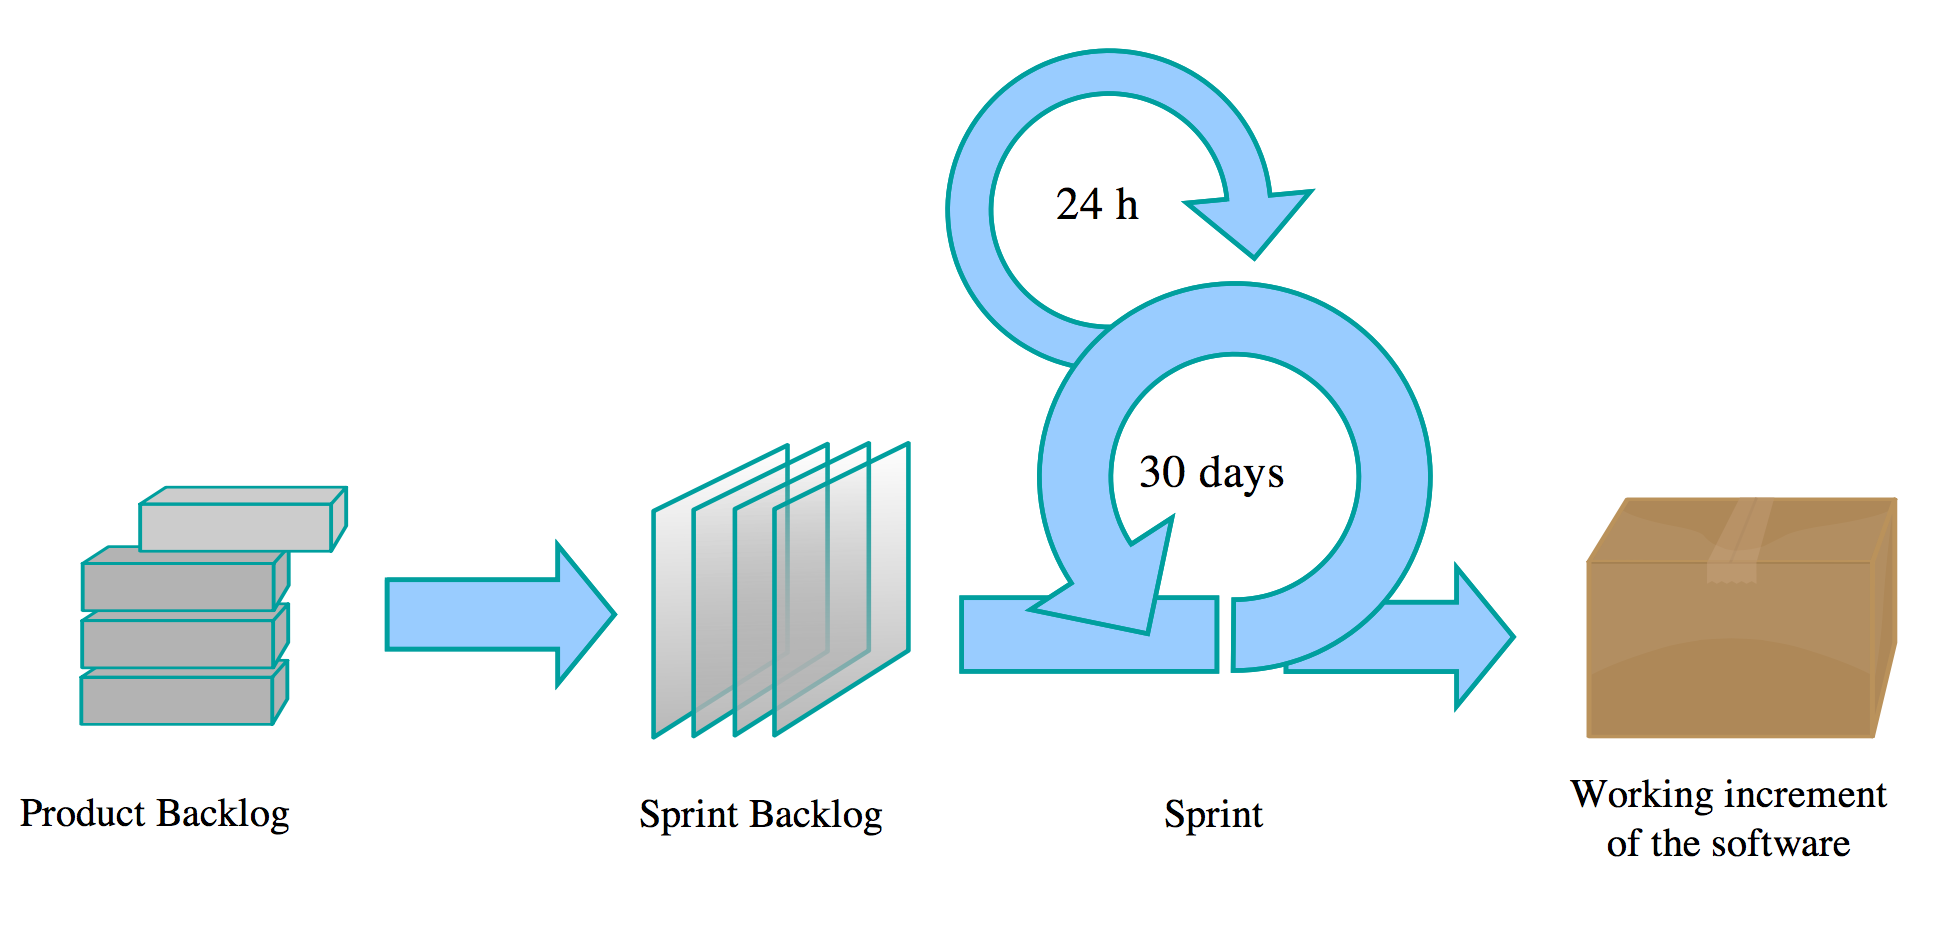
\includegraphics[width=150mm]{images/chapters/development_models/Scrum.png}
\caption{The Scrum cycle.}
\label{scrum}
\end{figure}

To end the section, as well as making a natural shift towards the next topic (Coordination), a look at Scrum-of-Scrums is carried out. It is a natural shift because Scrum-of-Scrums are used as the coordination mechanism across teams in the Scrum methodology. It works as the daily scrums (though usually implemented on a weekly basis because of time constraints and the complexity to find common times for all teams), but with one member assigned from each Scrum team to report completions, next steps and impediments for their respective teams. It is important that these impediments focus on the challenges that may impact coordination across teams and might limit other teams' work. The Scrum-of-Scrums will have their own backlog aiming to improve the cross-team coordination \cite{Sutherland2001}. Below the suggested questions for the SoS meetings are listed \cite{Cohn2007}:

\begin{enumerate}
  \item What did your team do since the previous meeting that is relevant to some other team?
  \item What will your team do by the next meeting that is relevant to other teams?
  \item What obstacles does your team have that affect other teams or require help from them?
  \item Are you about to put something in another team's way?
\end{enumerate}

Takeuchi et al. identified three strategies for distributed Scrum teams. The first type is isolated Scrum teams where teams operate as silos and no collaboration across teams is performed violating the agile principles. The second type is Scrum-of-Scrums which means overlapping Scrum teams. Here teams coordination, communicate and collaborate across teams through SoS meetings with participants from each team involved. Lastly, totally integrated Scrum teams are suggested. In this type teams are fully distributed and each team has members located at several sites. This approach creates similar characteristics as co-location. Type B is what is most common when several Scrum teams work together. The different types are visualised in figure \ref{distributedscrum} \cite{takeuchi2004}.

\begin{figure}
\centering
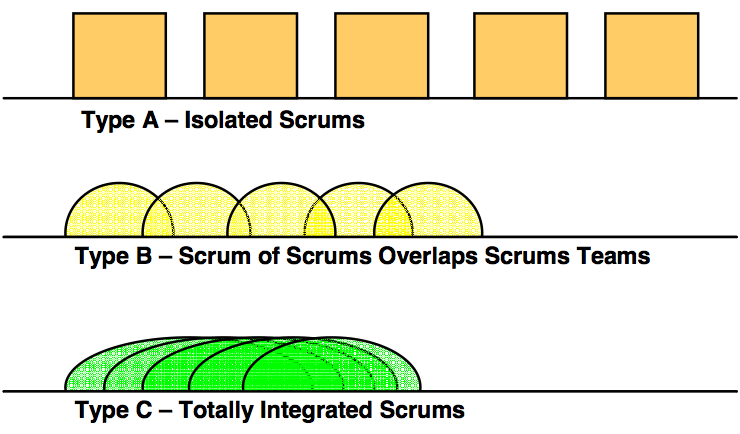
\includegraphics[width=110mm]{images/distributed_scrum.png}
\caption{Different strategies for distributed Scrum teams.}
\label{distributedscrum}
\end{figure}

\subsubsection{Kanban and Scrumban}
%Anderson

Kanban is a logistic control system that is closely related to lean software development. The word ``Kanban'' comes from two Japanese words: ``kan'' meaning visual and ``ban'' meaning board. The system was developed by Taiichi Ohno, an industrial engineer at Toyota. The reasoning behind developing this new system was to achieve and maintain a high level of production.

%http://link.springer.com/chapter/10.1007%2F978-3-642-20677-1_9
%Short description of Lean?

Cocco et al. described Kanban as the process of breaking down work to work items which are descriptions on cards (often post-it notes). These cards are then made visible for the entire team on a board. The board is used to show the flow of work within the team (or project). The high visibility comes from the cards and board showing which tasks are assigned to which member, communication priorities and highlights possible obstacles. An important feature of the Kanban method is to minimize Work in Progress (WIP) by reducing the amount of work items (cards) being developed at a time. This is done so the developers and customer can focus on smaller amounts, and should lead to an optimised process, as well as a reduced lead time. Compared to the Scrum methodology, Kanban (being a lean method) is able to release new futures more constantly, and not only at the end of each sprint iteration. Scrum is not able to change the requirements and direction of development in the middle of a sprint iteration, which Kanban can.

To get a more simplistic explanation of how the Kanban methodology works we can look at a standard work flow example. If a developer start on a task he moves this task from the ``work to be done'' section into the so-called ``work in progress'' column of the Kanban board. If there for some reason is a dependence towards other's work this particular work has to be moved to the ``on hold'' or ``waiting'' section of the board until the dependence is solved. After a task is completed it is moved into the final section of the board called the ``completed'' section. Teams also often use different colours to express the priority of the task, and tasks are often allocated to some specific part of the development, e.g., development, test etc. 

%TODO: Add kanban board?

%TODO: http://www.aboutscrumban.com/comparison-of-scrum-kanban-and-scrumban/
%TODO: http://www.aboutscrumban.com/

In later years a new approach has slowly surfaced which combines the Scrum and Kanban practices. This new methodology has been coined ``Scrumban'' (also referred to as ``Scrum-ban'' and ``Scrum ban''). The reasoning behind the evolution of this new methodology was that some practitioners felt that Scrum and Kanban did not fit all aspects of their work on their own with Scrum being too strict for constant change and releases (fast paced environments), and Kanban not being structured enough. The combination of the two methodologies is suppose to create a practice that fits a fast paced development environment. To get a better overview of the differences between Scrum, Kanban and Scrumban table \ref{coskas} is included.

\begin{center}
    \begin{longtable}{| p{2.6cm} | p{3.9cm} | p{3.9cm} | p{3.9cm} |}
   
    \hline & \textbf{Scrum} & \textbf{Kanban} & \textbf{Scrumban} \\ \hline
    \endfirsthead

    \multicolumn{4}{c}%
{{\bfseries \tablename\ \thetable{} -- continued from previous page}} \\ \hline
   & \textbf{Scrum} & \textbf{Kanban} & \textbf{Scrumban} \\ \hline
    \endhead

    \multicolumn{4}{|r|}{{Continued on the next page\ldots}} \\ \hline
    \endfoot

   \endlastfoot 

    \textbf{Iterations} & 1-4 week sprints & Continuous work alongside releases shorter than one week or bigger iterations like goals & Continuous work with short cycles for planning and longer cycles for release \\ \hline
    \textbf{Work routines} & Push and pull principle mixed with early binding to team members & Pull principle with late binding to team members & Pull principle with late binding to team members \\ \hline
    \textbf{Scope limits} & Sprint limits total work amount & Work in progress limits current work amount & Work in progress limits current work amount \\ \hline
    \textbf{Planning routines} & Sprint planning & Release/iteration planning, demand planning & Planning on demand for new tasks \\ \hline
    \textbf{Estimation} & Must be done before start of sprint & Optional & Optional \\ \hline
    \textbf{Performance metrics} & Burndown & Cumulative flow diagram, lead time cycle time & Average cycle time \\ \hline
    \textbf{Continuous improvement} & Sprint retrospective & Optional & Short Kaizen (continuous improvement) event as an option \\ \hline
    \textbf{Meetings} & Sprint planning, daily scrum, retrospective & Can be avoided & Short Kaizen event \\ \hline
    \textbf{Roles} & Product owner, Scrum master, team & Team and other work specific roles & Team and other work specific roles \\ \hline
    \textbf{Team members} & Cross-functional team members & Cross-functional team members, specialization is allowed & Specialization or preference to tasks \\ \hline
    \textbf{Task size} & The size that can be completed in sprint & Any size & Any size \\ \hline
    \textbf{New items in iteration} & Forbidden & Allowed whenever queue allows it & Allowed whenever queue allows it \\ \hline
    \textbf{Ownership} & Owned by a team & Supports multiple teams ownership & Supports multiple teams ownership \\ \hline
    \textbf{Board} & Defined/reset each sprint & Persistent & Persistent \\ \hline
    \textbf{Prioritization} & Through backlog & Optional & Recommended on each planning \\ \hline
    \textbf{Roles} & Scrum master, product owner, team & Not defined, may vary & Not defined, may vary \\ \hline
    \textbf{Rules} & Constrained process & Only a few constraints, flexible process & Slightly constrained process \\ \hline
    \textbf{Fit for} & Enterprise maturity for teams working on product or especially project which is longer than a year & Support and maintenance teams, continuous product manufacturing & Startups, fast-pace projects, continuous product manufacturing \\ \hline 

    \caption{Comparison of Scrum, Kanban and Scrumban}
    \label{coskas}
    \end{longtable}
\end{center}

%CEEOL (lasted ned artikkel)
%http://leansoftwareengineering.com/ksse/scrum-ban/
%http://en.wikipedia.org/wiki/Scrum_ban

\subsubsection{Pair programming}

Pair programming is a common practice in software development where two developers work side-by-side on the same computer, continuously collaborating and communicating on the same code. The thought behind the practice is to realise several potential benefits, such as:

%http://collaboration.csc.ncsu.edu/laurie/Papers/XPSardinia.PDF
%http://cacm.acm.org/magazines/2000/5/7671-all-i-really-need-to-know-about-pair-programming-i-learned-in-kindergarten/fulltext
%http://citeseerx.ist.psu.edu/viewdoc/download?doi=10.1.1.258.7427&rep=rep1&type=pdf

\begin{itemize}
  \item Production speed is faster in the long-term, and the pair comes up with a larger amount of possible solution than two developers working individually. This is called the ``pair programming advantage''.
  \item Code and general design quality is a lot higher (few bugs and defects). This is called the ``pair defect advantage''.
  \item Better job-satisfaction working in pairs than alone.
  \item Pair programming increases learning as knowledge is constantly shared between the two programmers.
  \item As developers are so tightly coupled in pair programming the team-building and communication improves.
\end{itemize}

There are three possible types of pairings in pair programming. These are explained below with their potential benefits and drawbacks:

\begin{itemize}
%http://www.sciencedirect.com/science/article/pii/S1071581906000644
  \item \textbf{Senior-Senior:} With two experts conducting the pair programming together this would in theory be the most productive pairing leading to the best results, however, such a pairing has shown to often cause problems as the seniors are less likely to question established practices.
%Williams, L. and Kessler, R. (2003). Pair Programming Illuminated. Boston: Addison-Wesley Professional.
  \item \textbf{Senior-Junior:} With a combination of both a senior and a junior developer often new ideas and solution surface as the junior programmer is more likely to question established practices, also leading to senior developers having to think through these practices. It is however important that the junior developer does not take an observer role, but is involved in the coding with the expert.
%http://collaboration.csc.ncsu.edu/laurie/Papers/XPSardinia.PDF
  \item \textbf{Junior-Junior:} The last pairing has two novice developers collaborating. Results have shown that two junior programmers working together yield better results than the two developers working separately, and is often used in academic settings.
\end{itemize}

\section{Coordination}

This section takes a look at different publications on coordination. It starts of with Malone and Crowston's well-known coordination theory. After this has been described a closer look at Strode's theoretical model of coordination is outlined. Ending the chapter is a brief look at the complexity factor introduced with a large-scale context in coordination.

\subsection{Malone and Crowston's Coordination Theory}

One of the most well-known papers on coordination theory was published by Malone and Crowston in 1990 and further redefined in 1994 (the focus will be on this paper) \cite{Malone1994}. Their study spanned different fields and can therefore be seen as an interdisciplinary coordination study. They listed an extensive amount of different definitions of coordination, and through these proposed definitions come up with a rather simple definition:

\begin{fancyquotes}
Coordination is managing dependencies between activities.
\end{fancyquotes}

These dependencies can occur when some task has to be postponed or extended because of its connection to another task, resource or unit. Their theory is based on a combination of coordination from several different disciplines such as computer science, organization theory, operations research, economics, linguistics, and psychology. They state that coordination consists of one or more coordination mechanisms, and that each of these address one or more dependencies.

While Strode et al. acknowledges their coordination theory as very useful for identifying these so-called dependencies, categorising them, and identifying coordination mechanisms in a situation, they conclude that it is only a theory for analysis and not intended to be used for prediction. Despite this being true, and the coordination theory not being suitable for predicting outcomes such as coordination effectiveness, their theory adds important information for better understanding of how activities or artefacts support coordination in organisational settings \cite{Strode2012}.

\subsection{Mintzberg's Coordination Mechanisms}

%TODO: Mintzberg, H.: Mintzberg on Management: Inside Our Strange World of Organizations (1989)

Around the 1980s Mintzberg performed well-known studies on organisational structures focusing on the division of labour into tasks to be carried out, and the coordination of these tasks to complete the activity. With this research six coordination mechanisms were identified in which organisations can coordinate their work:

\begin{itemize}
  \item In \textbf{direct supervision} there is typically one person, e.g., a manager, giving orders to other members and with that coordinating their work.
  \item In the \textbf{standardisation of work processes} coordination of the work happens through standards such as guidelines, orders, rules and regulations.
  \item In the \textbf{standardisation of outputs} the work is coordinated by performance standard measures of the outputs of the work.
  \item In the \textbf{standardisation of skills} coordination happens through standardisation of skills and knowledge, typically before the personnel starts performing the work.
  \item In the \textbf{standardisation of norms} it is the norms that are used to coordinate, meaning all members operate according to the same beliefs.
  \item In \textbf{mutual adjustment} the members coordinate their own work by informal communication with each other.
\end{itemize}

For agile software development it is in particular the mutual adjustment mechanism that is present. Because of its nature it is well suited for complex, dynamic and innovative environments. With the large focus on rapid and continuous delivery the use of informal communication arenas are to a great degree existent in agile software development.

\subsection{Strode's Theoretical Model of Coordination}
\label{strodechap}

Strode et al. performed a multi-case study on three different co-located agile projects in 2012 \cite{Strode2012}. From these projects the findings led to a theoretical model of coordination that will be outlined in this section. It is important to note that these projects were not large-scale.

From these case studies three main components for the theoretical model were extracted: Synchronisation, Structure and Boundary Spanning. These components combine to what is called the ``Coordination Strategy''. Coordination strategy is in this context a group of coordination mechanisms that manage dependencies in a situation. The theoretical model of coordination can be seen in figure \ref{strode}. Below the three main components will be explained in more detail:

\begin{figure}
\centering
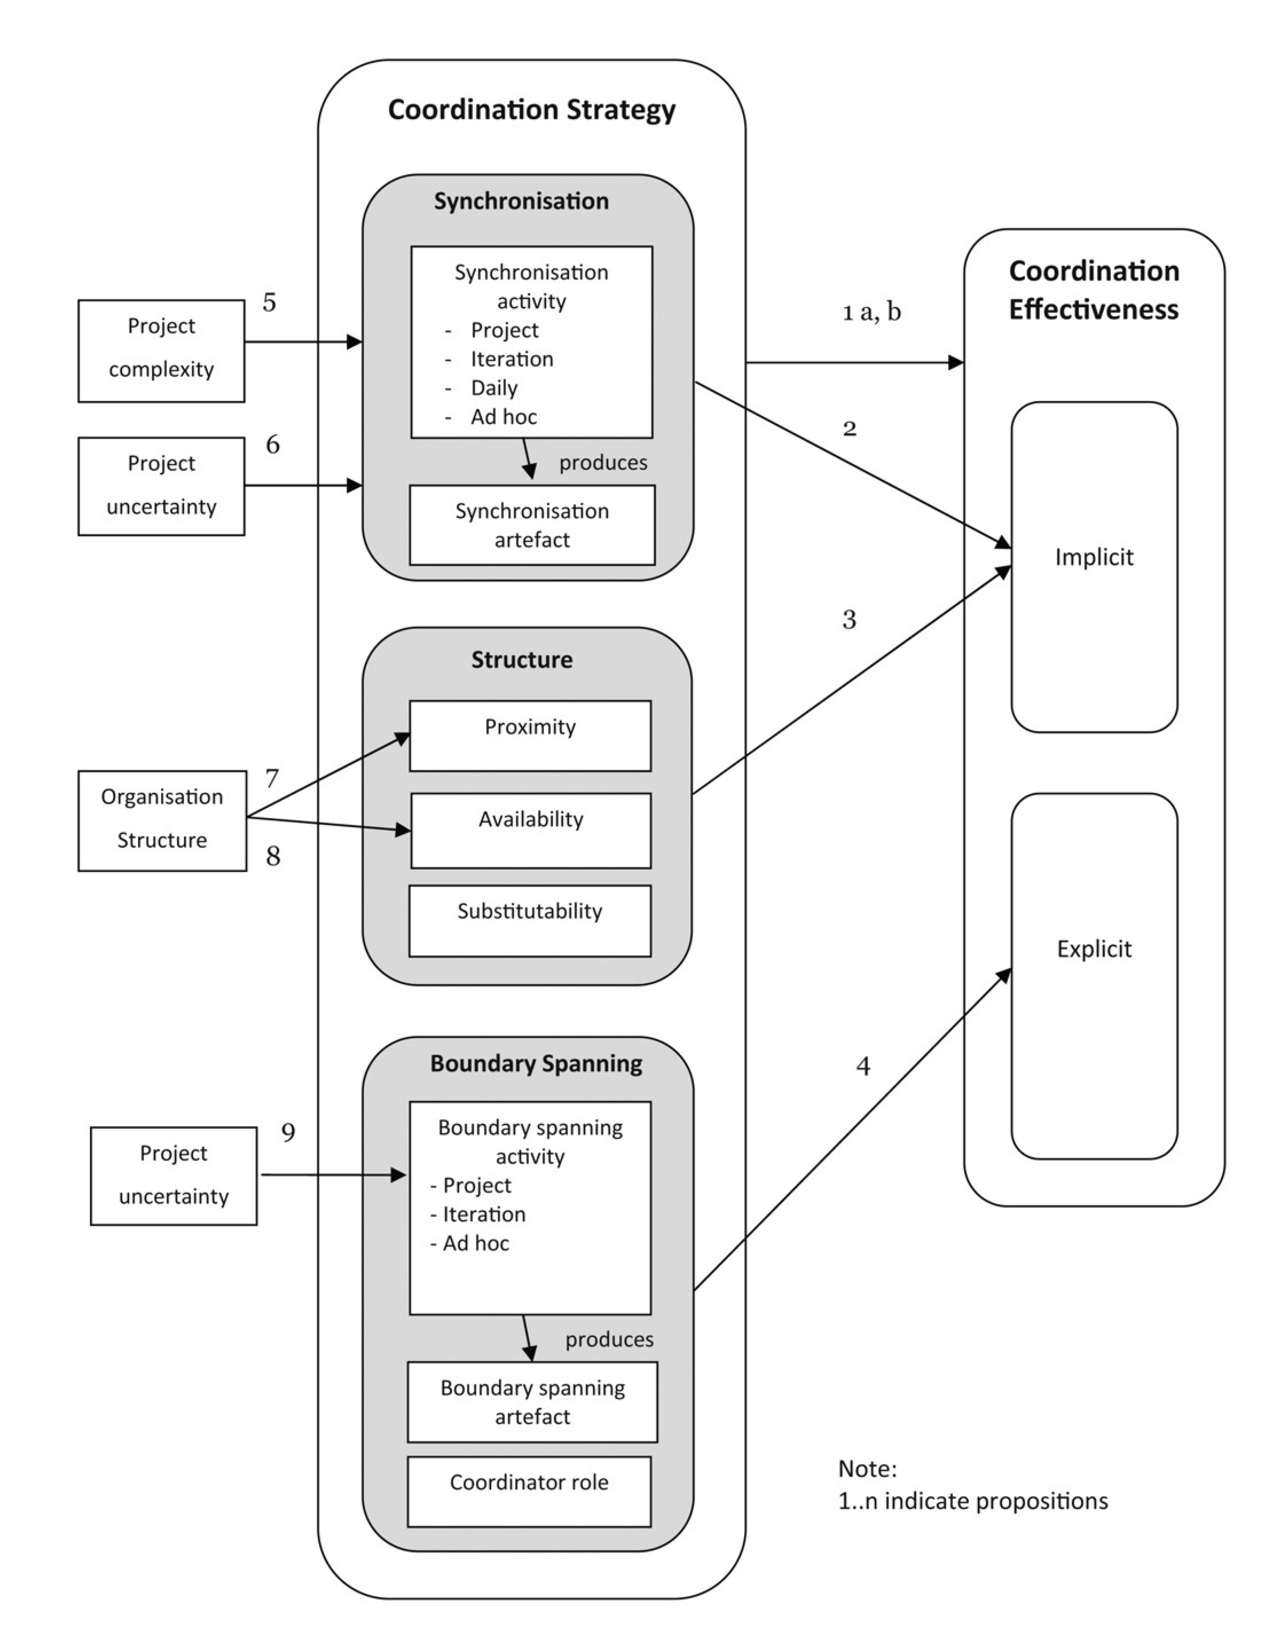
\includegraphics[width=160mm]{images/Strode.pdf}
\caption{A theory of coordination in agile software development projects.}
\label{strode}
\end{figure}

\subsubsection{Synchronisation}

Synchronisation in this context consists of synchronisation activities and synchronisation artefacts produced and used during these activities. Synchronisation activities are activities performed by all team members simultaneously. They contribute to a common understanding of the task, process, and or expertise of other team members. Synchronisation artefacts on the other hand are artefacts that are generated during synchronisation activities. These artefacts may be visible for the entire team or largely invisible but available. The artefacts can take a physical or virtual form, and are temporary or permanent.

\subsubsection{Structure}

Structure in this model is the arrangement of, and relations between, the parts of something complex. It consists of three categories: proximity, availability and substitutability. Proximity is the physical closeness of other (individual) team members. Availability means that other team members are accessible for requests or information. Lastly, substitutability has to do with the team members ability to perform others' work to maintain time schedules.

\subsubsection{Boundary Spanning}

The last component of the coordination strategy is boundary spanning. Boundary spanning has to do with the interaction with other organisations or other business units that are not involved in the project. It consists of three aspects: boundary spanning activities, boundary spanning artefacts and a coordinator role. Boundary spanning activities are activities performed to achieve help from some unit or organisation not involved in the project. The boundary spanning artefacts are artefacts produced to enable this external coordination. These artefacts have the same characteristics as synchronisation artefacts. Lastly, the coordinator role is a role taken by someone within the project team. His or her role is to support interaction to outside personnel to extract resources or information needed in the project at hand.

\subsubsection{Coordination Effectiveness}
\label{strode_ce}

There is another important part of the theoretical model of coordination, namely the coordination effectiveness concept. This concept will be further explained in section \ref{efficiency} that takes a look at coordination effectiveness.

\subsubsection{Propositions}

There are in total ten propositions (Proposition 1 has two parts) linking the coordination concepts in Strode's theoretical coordination model showed in figure \ref{strode}. These are outlined below:

\begin{fancyquotes}
\textbf{Proposition 1a:} A coordination strategy that includes synchronisation and structure coordination mechanisms improves project coordination effectiveness when the customer is included in the project team. Synchronisation activities and associated artefacts are required at all frequencies – project, iteration, daily, and ad hoc.
\end{fancyquotes}

\begin{fancyquotes}
\textbf{Proposition 1b:} A coordination strategy that includes synchronisation, structure, and boundary spanning coordination mechanisms improves project coordination effectiveness when the customer is an external party to the project. Synchronisation activities and associated artefacts are required at all frequencies – project, iteration, daily, and ad hoc. Boundary spanning activities and associated artefacts are required at all frequencies – project, iteration, and ad hoc.
\end{fancyquotes}

\begin{fancyquotes}
\textbf{Proposition 2:} Synchronisation activities at all frequencies – project, iteration, daily, and ad hoc, along with their associated synchronisation artefacts, increase implicit coordination effectiveness.
\end{fancyquotes}

\begin{fancyquotes}
\textbf{Proposition 3:} Structural coordination mechanisms i.e. close proximity, high availability, and high substitutability, increase implicit coordination effectiveness.
\end{fancyquotes}

\begin{fancyquotes}
\textbf{Proposition 4:} High levels of boundary spanning coordination mechanisms, i.e. boundary spanning activities at all frequencies – project, iteration, and ad hoc, their associated boundary spanning artefacts, and a coordinator role, increases explicit coordination effectiveness.
\end{fancyquotes}

\begin{fancyquotes}
\textbf{Proposition 5:} Under conditions of high project complexity, increasing the frequency of iteration and ad hoc synchronisation activities will maintain coordination effectiveness. The production of related synchronisation artefacts must be adjusted accordingly.
\end{fancyquotes}

\begin{fancyquotes}
\textbf{Proposition 6:} Under conditions of high project uncertainty, to maintain synchronisation activity frequency and production of associated artefacts, changing the priority of stories will maintain coordination effectiveness.
\end{fancyquotes}

\begin{fancyquotes}
\textbf{Proposition 7:} A mono-project organisation structure enables close proximity relative to multi- or matrix structures.
\end{fancyquotes}

\begin{fancyquotes}
\textbf{Proposition 8:} A mono-project organisation structure improves availability relative to multi- or matrix style structures.
\end{fancyquotes}

\begin{fancyquotes}
\textbf{Proposition 9:} Under conditions of high project uncertainty, when the customer is not part of the team, increased boundary spanning coordination mechanisms will maintain coordination effectiveness. The production of related boundary spanning artefacts must be adjusted accordingly.
\end{fancyquotes}

\subsection{Coordination in Large-scale}
\label{largescalecor}

This section takes a closer look at general studies performed on large-scale coordination and is not specifically focusing on software development. The section is added to highlight the introduction of complexity that a large-scale context brings with it.

Van der Ven et al. released an article in 1976 where they tried to identify determinants of coordination modes within organisations. They state that an increase in size will produce a trade-off between the increasing complexity and cost of coordination at the administrative level. From the research two different coordination forms are described, namely vertical and horizontal. The vertical communication includes coordination through curators, while the horizontal communication occurs by way of one-to-one communication. Their findings show that when team size increases the coordination moves towards a more vertical and impersonal style \cite{Ven1976}. This is backed up by John Child in a publication from 1973. Here he states that with a growing complexity level there is likely that administrative problems will occur regarding coordination and control \cite{Child1973}.

\section{Large-scale}

Having looked at coordination in large-scale in section \ref{largescalecor}, what is actually this so-called ``large-scale''? This was a topic brought up at a workshop regarding research challenges in large-scale agile software development where opinions regarding how large-scale should be defined varied a lot. Some suggestions were to define it through project duration, project cost, number of people involved, number of remote sites and/or number of teams \cite{Dingsoyr2013b}. This issue was further analysed by Dingsøyr, Fægri and Itkonen trying to work out a taxonomy of scale for agile software development. Their results are summarised in table \ref{Scale} where the taxonomy of scale is based on the amount of teams involved in the development project \cite{Dingsoyr2013a}.

\begin{table}
\begin{center}
    \begin{tabular}{| l | l | p{7cm} |}
    \hline
    \textbf{Level} & \textbf{Number of teams} & \textbf{Coordination approaches} \\ \hline
    Small-scale & 1 & Coordinating the team can be done using agile practices such as daily meetings, common planning, review and retrospective meetings. \\ \hline
    Large-scale & 2-9 & Coordination of teams can be achieved in a new forum such as a Scrum of Scrums forum. \\ \hline
    Very large-scale & 10+ & Several forums are needed for coordination, such as multiple Scrum of Scrums. \\
    \hline
    \end{tabular}
    \caption{A taxonomy of scale of agile software development projects.}
    \label{Scale}
\end{center}
\end{table}

Others have also discussed problems regarding large-scale. For example Schnitter and Mackert discuss the scaling of Scrum at SAP AG and concludes that in their case the maximum involved development employees that may be organised with regards to agile project management is 130 (This number sums up developers in 7 teams (max. 70 people), the product team (max. 16), development infrastructure responsible (about 10), quality assurance and testers (about 25), general management (about 10)) \cite{Nord2011}.

Another example is taken from Nord et al. defining large-scale by scope of the system, team size, and project duration. They say that the size of the development team must be more than 18 people and distributed into a few teams \cite{Robert2014}.

So the definition of a ``large-scale agile project'' used in this research will be:

\begin{fancyquotes}
An agile project must consist of a minimum amount of two teams coordinating across the teams to be categorised as large-scale.
\end{fancyquotes}

\textbf{ }

\section{Multiteam Systems}
%TODO: Ha med referanse til tidligere?
%TODO: Cites i avsnitt
As mentioned earlier the work environments have become more challenging and complex in line with the growth of communication and information technology. This growth has led to the globalisation of organisational work. With the globalisation an increase in interconnectivity across organisational boundaries has become apparent. Because of this trend new questions and problems have surfaced. Unfortunately, these questions and problems have not been possible to adapt to traditional organisational forms. This has led to the introduction of new and different organisational forms, e.g., matrix and virtual organisations, and cross-functioning and ad hoc project teams. One of these new organisational forms focus on projects where collaboration exists across traditional team and organisational boundaries. This form does not resemble traditional organisations or large-scale teams, but can be seen as an aggregation that includes tightly coupled arrangement of teams, where the different teams may have noticeable different norms, expertise, missions, structures and operating procedures to the overall work. Mathieu, Marks, and Zaccaro \cite{TODO} defined the organisations corresponding to the aforementioned form as multiteam systems (MTSs). Below their definition follows:

\begin{fancyquotes}
Two or more teams that interface directly and interdependently in response to environmental contingencies towards the accomplishment of collective goals. MTS boundaries are defined by virtue of the fact that all teams within the system, while pursuing different proximal goals, share at least one common distal goal; and in doing so exhibit input, process and outcome inter-dependence with at least one other team in the system \cite{TODO}.
\end{fancyquotes}

From this definition it is easy to see similarities with so-called ``large-scale'' projects and organisations. Both large-scale projects' and multiteam systems' taxonomies look at the amount of teams involved, where the minimum number is two, but are typically larger than this number by a considerable margin. In both categories the teams have to be somewhat interconnected, and the organisational boundaries may be crossed, meaning teams can reside in different organisations. Mathieu et al. have therefore categorised MTSs into ``internal MTSs'' where the whole system or project is situated within an organisation, and ``cross-boundary MTSs'' where teams are located in different organisations, hence organisational boundaries have to be crossed to achieve collaboration \cite{TODO}.

One of the most distinguishing factors of multiteam systems is their focus on goal hierarchies. As mentioned above interdependencies are not only witnessed within teams, but also across them. From the definition of MTSs the teams have different proximal goals, but all share at least one distal goal. Mathieu et al. define the feature of these goal hierarchies that are relatively common across different MTSs as:

\begin{enumerate}
  \item MTS goal hierarchies have a minimum of two levels
  \item Goals at higher levels entail greater interdependent actions among more component teams than goals at lower levels
  \item The superordinate goal at the apex of the hierarchy rests on the accomplishment by component teams of all lower order goals
  \item Higher order goals are likely to have a longer time horizon than lower order goals
  \item Goals vary in their priority and valence
\end{enumerate}

%TODO: Skrive om ulike typer interdependencies?

\subsection{MTS Characteristics}

Having looked at the features of multiteam systems the attention is shifted towards their attributes. These attributes are what separates different MTSs. The attributes are classified into three dimensions, compositional, linkage and development attributes, and will be presented in the following sections. The different dimensions are summarised in table \ref{domsc}.

\subsubsection{Compositional Attributes}

In the compositional dimension several demographic features of the MTS and characteristics of component teams are looked at. In total there are ten attributes, and these will be outlined in this section. Regarding the magnitude of the MTSs two attributes are used. Firstly the ``number'' of component teams located within the MTS, and secondly the total ``size'' of the MTS, meaning the amount of individual members involved in the multiteam system.

%Skrive om problemer som kan oppstå når det blir for mange team/medlemmer?

Another compositional attribute that was earlier mentioned as a distinguishing factor is ``boundary spanning''. This attribute is concerned with where the different component teams originate from. If all component teams come from the same organisation it is an internal MTS, while if the component teams come from two or more organisations it is an external MTS. External MTSs are more complex and are more likely to run into task and social complexity than its counterpart. In this context, social complexity refers to diversity, scale, scope, and dynamism of stakeholders in the MTS's environment \cite{?}. There are two more attributes concerned with boundary spanning which are at a higher detail level. Firstly the ``organisational diversity'' looks at the total amount of organisations represented in the MTS. With a higher number of organisations the likelihood of a higher level of social complexity rises. Secondly the ``proportional membership'' outlines the percentage of teams from different organisations. With an unbalanced proportional membership there is a risk that the influence level will be greater from the organisation(s) with the highest amount of teams.

%TODO: Usikker på om det er i teams eller mellom teams det er snakk om?
The sixth compositional attribute is concerned with how similar the different component teams' core task and goals are. This attribute is called ``functional diversity''. With an increase in this so-called functional diversity problems may occur. Another important factor in MTSs is ``geographic dispersion''. There are three degrees of geographical dispersion, namely co-located, partially co-located, and fully dispersed. Some problems that have been witnessed in dispersed projects has been communication issues, coordination difficulties and trust building. Building on the geographic dispersion is an attribute called ``cultural diversity''. If teams are dispersed and the boundaries extend the national borderline this could lead to cultural clashes.

The ninth attribute in the compositional dimension is ``motive structure''. This attribute refers to the degree to which the different teams commit to the MTS, and how compatible and closely linked the team goals and the MTS goals are. A problem that can occur in this compositional attribute is that a team's proximal and/or distal goals are in conflict with the overall goals of the MTS leading to more complex interteam processes. With an increase in incompatibility in goals between the MTS and the compositional team(s) this can lead to team members being less committed to the overall goal hierarchy of the multiteam system. Motive structure may be associated with the last compositional attribute called ``temporal orientation''. Temporal orientation is concerned with the amount of resources dedicated to the MTS by each component team.

As can be seen the compositional attributes are important factors in interteam dynamics within MTSs. Focus on team composition is important to keep the level of effectiveness high, as well as prohibiting evolution of subgroups.

\subsubsection{Linkage Attributes}

Moving on the focus is shifted towards the so-called linkage dimension. Linkage mechanisms and attributes are concerned with how teams are arranged and connected within a multiteam system. The first attribute is concerned with the amount of coordination between different component teams that is needed and is called ``interdependence''. The degree of interdependence will differ from different MTSs, but with an increasing interdependence the amount of interteam processes necessary will increase to achieve high MTS effectiveness.

Two other linkage attributes that often correlate are ``hierarchical arrangement'' and ``power distribution''. Hierarchical arrangement focuses on how teams are organised within the MTS with regards to their responsibility level of goal attainment. The more proximal goals the component team is involved with, the higher in the hierarchical arrangement they are. As for power distribution the focus is on the relative influence that component teams have within a multiteam system. Often the teams placed higher in the hierarchical arrangment, meaning they have more proximal goals, also have a bigger influence and power. Other factors that could lead to higher power can be team size, the team's functional centrality to the core mission of the MTS, and/or the parent organisations having assigned the team with authority. Both attributes will likely influence communication, interaction and collaboration between the component teams in a multiteam system.

Moving on to the forth and fifth linkage attributes the focus is shifted towards the communication structures of MTSs. Firstly ``communication networks'' refer to the most common interaction and communication patterns between and within component teams. These networks can be fully decentralised (everyone interactive with everyone), fully centralised (everyone communicate to and through one single member of the MTS), and various patterns between these two boundary points. It is important to notice that the chosen communication network in a multiteam system will have a great impact on the task efficiency of the MTS. Lastly ``communication modality'' is concerned with which modes are used to communicate across component teams within a multiteam system. These can be, e.g., face-to-face interaction, electronic communication, or a mixture of the two. Often the degree of which modes are used is closely linked to the aforementioned compositional attribute called ``geographic dispersion''. With co-located teams preferring a higher amount of face-to-face communication.

\subsubsection{Developmental Attributes}

The last dimension of multiteam systems is the developmental. Developmental attributes are concerned with the developmental dynamics and patterns of MTSs. The first attribute looks at how the MTS was put to life, its ``genesis''. The origin of MTSs can either occur through appointment from parent organisations, or they may emerge from collective initiative of several teams. The type of genesis can have an impact on different aspects of a MTS, e.g., the distal goal. Another developmental attribute is ``direction of development'' and looks at the direction the MTS takes from its origin. For example the MTS could have emerged from a specific event, but then move towards a more formalised entity as time passes. Another development path could be the MTS being formally planned in anticipation of a possible situation occurring, but when the event does occur acctually evolve in membership and linkages.

Two other developmental attributes are ``tenure'' and ``stage''. The tenure attribute is concerned with the anticipated  duration of the MTS, while the stage attribute looks at which particular stage of development the MTS is in. Starting as a newly formed multiteam system it will evolve through different phases to finally becoming a mature MTS. The stage of MTS development will often give a hint to the efficiency of the MTS's interteam processes. 

%Skrive mer om hva som skjer når nye team kommer inn? Skrive mer om "adaptation"?
The last two developmental attributes together combine to the group term ``transformation of system composition'', meaning if there are changes to the composition as the MTSs develop and move through the different phases of development. The first of these focuses on ``membership constancy'' and refers to how constant or fluid the number of component teams are. Often in more complex and turbulent environments the amount of component teams may change over the course of the MTS's lifespan. Lastly ``linkage constancy'' is concerned with how the component teams are connected. The focus is on if these linkages between the component teams in a multiteam system is constant or if they change as the MTS progresses. Again the likelihood of fluidity in coordination structures between teams is higher when the MTS is located in more turbulent and dynamic environments.

In the above sections three dimensions of multiteam systems and their attributes have been presented. It is important to note how the different attributes can be factors in achieving effective MTSs and MTS processes. A simple model of MTS effectiveness is outlined in figure \ref{amomse}, where the attributes of the compositional, linkage and developmental dimensions can be seen as predecessors of different intrateam and interteam processes. The effects of these attributes on the total effectiveness of the multiteam system would be arbitrated by these intra- and interteam processes.

\begin{figure}
\centering
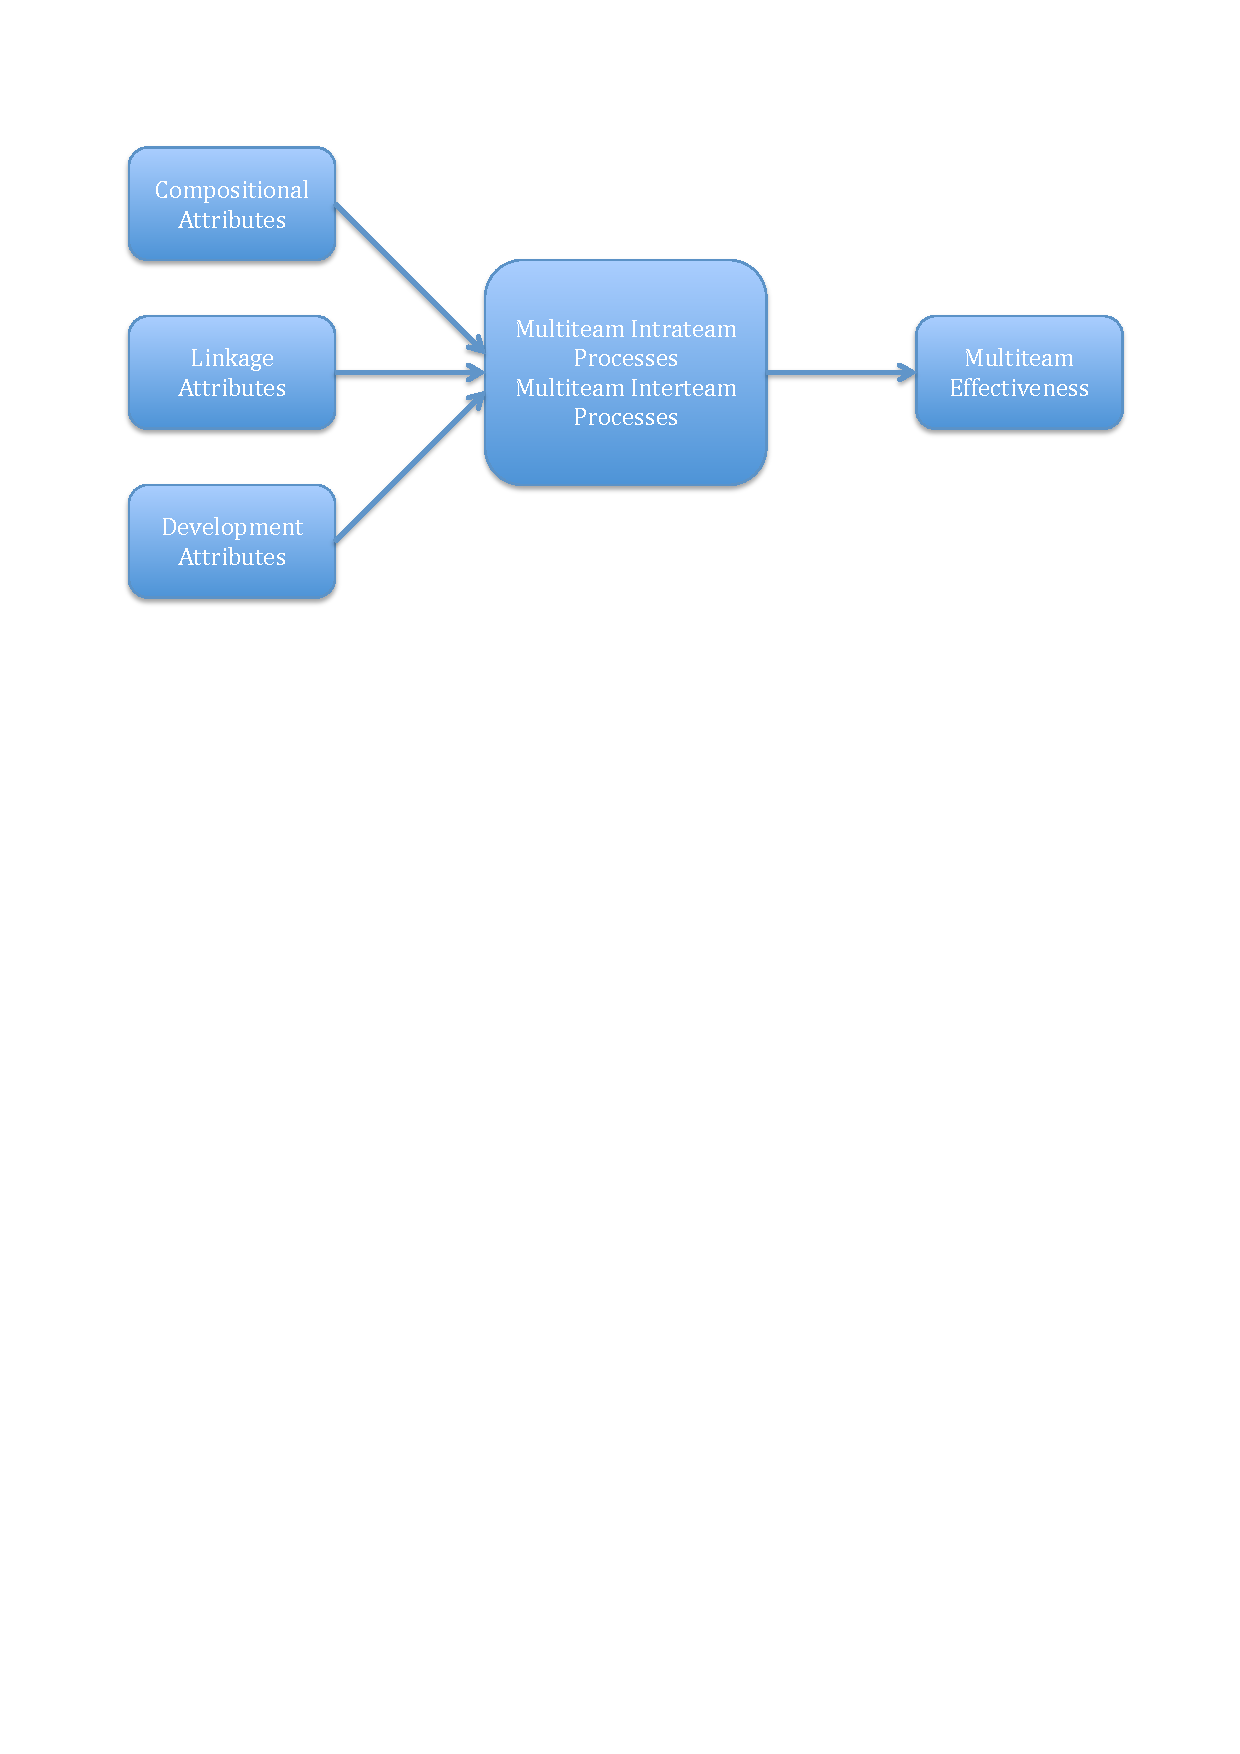
\includegraphics[trim = 15mm 190mm 15mm 10mm, width=150mm]{images/multiteam_system_model.pdf}
\caption{A model of multiteam system effectiveness.}
\label{amomse}
\end{figure}


%TODO: Fiks tabell
\begin{center}
\begin{longtable}{ | p{2.5cm} | p{4cm} | p{8cm} | }

   
    \hline \textbf{Dimension} & \textbf{Attribute} & \textbf{Explanation} \\ \hline
    \endfirsthead

    \multicolumn{3}{c}%
{{\bfseries \tablename\ \thetable{} -- continued from previous page}} \\ \hline
   \textbf{Dimension} & \textbf{Attribute} & \textbf{Explanation} \\ \hline
    \endhead

    \multicolumn{3}{|r|}{{Continued on the next page\ldots}} \\ \hline
    \endfoot

   \endlastfoot 

	\multirow{10}{*}{Compositional} & Number & Number of component teams within the MTS \\ \cline{2-3}
 	& Size & Total number of individual members across teams \\ \cline{2-3}
 	& Boundary status & Component teams come from single organization (internal) versus multiple organisations (external or cross-boundary) \\ \cline{2-3}
 	& Organisational diversity & In a cross-boundary MTS, the number of different organisations represented among the component teams \\ \cline{2-3}
	& Proportional membership & In a cross-boundary MTS, the percentage of teams from different organisations \\ \cline{2-3}
	& Functional diversity & Degree of heterogeneity in the core purposes and missions of component teams \\ \cline{2-3}
	& Geographic dispersion & Co-located or dispersed component teams \\ \cline{2-3}
	& Cultural diversity & Degree to which component teams come from different nations or cultures \\ \cline{2-3}
	& Motive structure & Degree of commitment of each component team to the MTS; the compatibility of team goals and MTS goals \\ \cline{2-3}
	& Temporal orientation & Level of effort and temporal resources expected of each component team \\ \cline{2-3}
\hline
	\multirow{5}{*}{Linkage} & Interdependence & Degree of integrated coordination (e.g., input, process, outcome) among members of different component teams \\ \cline{2-3}
 	& Hierarchical arrangement & Ordering of teams according to levels of responsibility \\ \cline{2-3}
 	& Power distribution & The relative influence of teams within the MTS \\ \cline{2-3}
	& Communication structure: Network & The typical patterns of interteam communication \\ \cline{2-3}
	& Communication structure: Modality & The modes of communication (e.g., electronic, face-to-face, or mixed) that occur across component teams \\ \cline{2-3}
\hline
	\multirow{6}{*}{Developmental} & Genesis & The initial formation of an MTS as either appointed or emergent \\ \cline{2-3}
 	& Direction of development & From emergent to formalised; an evolution from an early formal state \\ \cline{2-3}
	& Tenure & The anticipated duration of the MTS \\ \cline{2-3}
	& Stage & The stage of MTS development from newly formed to mature \\ \cline{2-3}
	& Transformation of system composition: Membership constancy & Fluidity versus constancy of component teams as members \\ \cline{2-3}
	& Transformation of system composition: Linkage constancy & Fluidity versus constancy of linkages among component teams \\ \cline{2-3}
	\hline
\caption{Dimensions of multiteam system (MTS) characteristics.}
\label{domsc}
\end{longtable}
\end{center}

\section{Efficiency, Effectiveness, Productivity and Performance in Coordination}
\label{efficiency}

There has been released a good amount of papers regarding effectiveness, productivity and efficiency in project literature. Unfortunately research in this area that focuses on large-scale is scarce. Therefore, the work highlighted in this section will mainly be extracted from small-scale studies. To start the section of a closer look at the aforementioned study by Strode et al. will be performed, before a summary of some different field studies on the matter will be carried out.

\subsection{Strode's Coordination Effectiveness}
\label{cordinationeffectiveness}

Part of the theoretical model of coordination by Strode et al. seen in figure \ref{strode} is the so-called ``coordination effectiveness''. This concept was developed by Strode et al. in 2011 having used the same three agile projects discussed earlier, as well as a non-agile software development project as a foundation \cite{Strode2011}. Coordination effectiveness is defined as the outcome of a particular coordination strategy. Coordination effectiveness is split into two components: an implicit and an explicit part.

The implicit part is concerned with coordination that occurs without explicit speech or message passing, this happens within work groups. It has five components: ``Know why'', ``Know what is going on and when'', ``Know what to do and when'', ``Know who is doing what'', and ``Know who knows what''. These aspects are pretty self-explanatory.

The explicit component on the other hand is concerned with the physical aspects of the project. It states that the objects involved in the project have to be in the correct place, at the correct time and in a state of readiness for use. A summary of the combination of explicit and implicit coordination effectiveness is provided in figure \ref{effectiveness}.

\begin{figure}
\centering
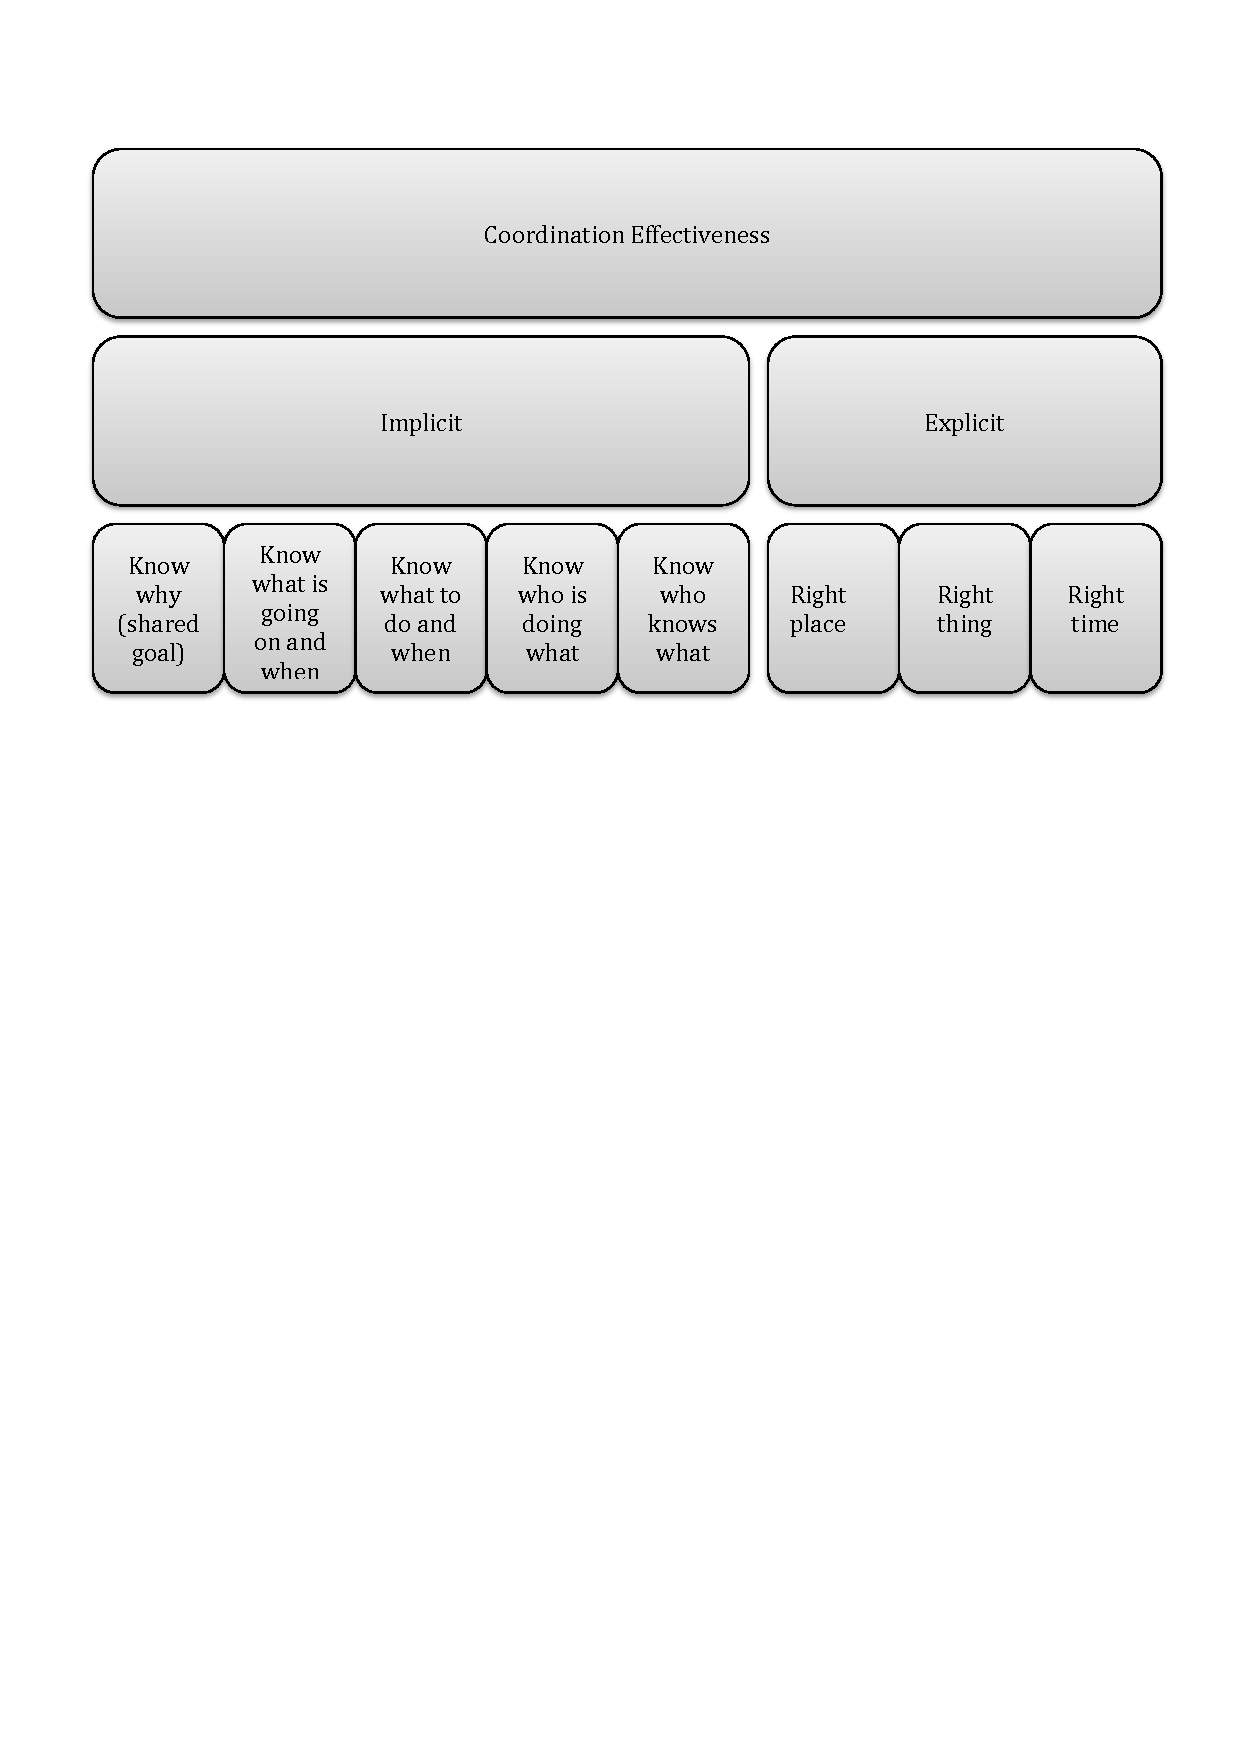
\includegraphics[trim=0cm 17.5cm 0cm 1.5cm, width=160mm]{images/Coordination_Effectiveness.pdf}
\caption{Components of coordination effectiveness from Strode et al. (2011).}
\label{effectiveness}
\end{figure}

To end this subsection a definition of coordination effectiveness from Strode et al. is provided:

\begin{fancyquotes}
Coordination effectiveness is a state of coordination wherein the entire agile software development team has a comprehensive understanding of the project goal, the project priorities, what is going on and when, what they as individuals need to do and when, who is doing what, and how each individuals work fits in with other team members work. In addition, every object (thing or resource) needed to meet a project goal is in the correct place or location at the correct time and in a state of readiness for use from the perspective of each individual involved in the project \cite{Strode2011}.
\end{fancyquotes}

\subsection{Some Studies on the Field}
\label{large_scale_coordination}

Below four studies that try to identify important factors of coordination's impact on team performance are described.

\subsubsection{Team Effectiveness 1997-2007: A Review of Recent Advancements and a Glimpse Into the Future}

Mathieu et al. takes a look at literature published on team effectiveness in a ten year period. They look at several different aspects regarding the nature of teamwork \cite{Mathieu2008}. It is important to note that the main focus of this article is on small-scale teams, and that the publications used are not gathered directly from the software and agile field. However, the article gives perspectives that are noteworthy. The main focal point here will be on Mathieu's chapter on organisational contexts, and the section on multi-team systems coordination in particular.

One aspect that was identified in several studies having a positive impact on performance was an ``openness climate''. What was concluded at the macro organisational level was that a support for an openness climate at the broader level of the organisation had a positive impact on team level processes.

Quite a few studies were identified on multi-team systems coordination as well. Here, the findings showed a positive correlation between inter-team coordination and intra-team coordination. Hyatt et al. indicated that teams perform more effectively as self-contained units when they have robust information networks, as well as communication and cooperation channels, both within and between teams \cite{Hyatt1997}. This again highlights the importance of studies focusing on coordination in large-scale.

\subsubsection{Interpretative Case Studies on Agile Team Productivity and Management}

Melo et al. performed a multi-case study on three large Brazilian IT companies that were using agile methods in their projects \cite{Melo2013}. The objective of the research was to provide a better understanding of which factors that had an impact on agile team productivity. To document teamwork effectiveness they used the well-known theoretical model ``Input-Process-Outcome'' (IPO). Their input factors were ``Individual and Group characteristics'', ``Stage of team development'', ``Nature of task'', ``Organizational context'' and ``Supervisory behaviors''. One process-category was identified: ``Group processes''. Lastly they identified two outcome-groups, namely ``Agile team productivity'' and ``Attitudinal and Behavioral''. All of these are summarised constituting the conceptual framework for their agile team productivity in figure \ref{atpcf}.

\begin{figure}
\centering
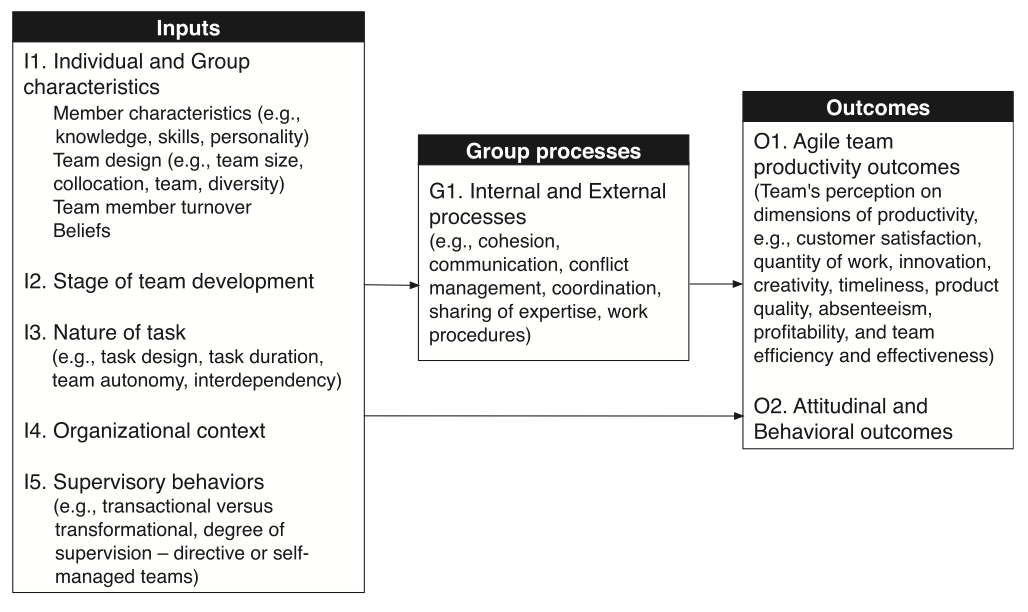
\includegraphics[width=150mm]{images/IPO.png}
\caption{Agile team productivity conceptual framework.}
\label{atpcf}
\end{figure}

After collecting the data from their multi-case study they mapped the results in a thematic map on agile productivity factors. These findings showed three main groups of team management and their impact on productivity. For this study it is the ``Inter-team coordination'' and ``Team design choices'' that are interesting because of their impact on coordination to a larger degree, meaning ``Team member turnover'' is left out. 

In ``Team design choices'' four roots of impact were identified: ``Team size'', ``Team members skills'', ``Team collocation'' and ``Team members allocation''. Out of these team collocation and team size seem to effect coordination effectiveness the most. Their findings showed that smaller teams led to better communication and alignment, while collocation had a positive influence on team productivity as it helped overcome invisible barriers between teams in a hierarchical company.

For ``Inter-team coordination'' two roots were identified: ``Lack of commitment among teams'' and ``Inappropriate coordination rules among teams''. One of the main reasons for negative impact was identified to be external dependencies because projects often were left waiting for results of entities outside the project team. So a problem in inter-team coordination was misalignment, hence, synchronisation is an important factor.

\subsubsection{Dispersion, Coordination and Performance in Global Software Teams: A Systematic Review}

Anh et al. performed a systematic literature review (SLR) to collect relevant studies on dispersion, coordination and performance in global software development (GSD), and highlighted the findings of impact factors in a thematic mapping \cite{Anh2012}. It is important to note that the findings are not from agile software development, but they are still interesting because of the global aspect in the literature used. The results are briefly summarised in table \ref{GSD}:

\begin{table}
\begin{center}
    \begin{tabular}{ | p{5cm} | p{8cm} |}
    \hline
    \textbf{Type} & \textbf{Impact on team performance} \\ \hline
    Presence of geographical dispersion & Negative (work takes longer time, less effective communication and coordination) \\ \hline
    Number of sites/Team size & Negative (complicates coordination and hampers communication) \\ \hline
    Large time zone differences between teams & Negative (creates coordination problems because of the complexity introduced) \\ \hline
    \end{tabular}
    \caption{Impact of geographical dispersion on performance.}
    \label{GSD}
\end{center}
\end{table}

\subsubsection{Team Performance in Agile Development Teams: Findings from 18 Focus Groups}

Dingsøyr and Lindsjørn carried out a focus group study looking at which factors the agile software practitioners in the research perceived as influential on effective teamwork \cite{Dingsoyr2013c}. This paper focuses on the team performance of individual teams, but is included because of its agile nature. To place the suggestions from the participants into categorise Dingsøyr et al. decided to use the ``Big Five'' model proposed by Salas et al. \cite{Salas2005} leading to eight teamwork components: ``Team leadership'', ``Mutual performance monitoring'', ``Backup behaviour'', ``Adaptability'', ``Team orientation'', ``Shared mental models'', ``Mutual trust'' and ``Closed-loop communication''. A summary of the distribution of all suggestions over these components is outlined in table \ref{summary2}.

\begin{table}
\begin{center}
    \begin{tabular}{ | p{6cm} | p{2.5cm} | p{2.5cm} | p{2.5cm} |}
    \hline
    \textbf{Teamwork component} & \textbf{Foster} & \textbf{Hinder} & \textbf{Total} \\ \hline
    Team leadership & 90 & 139 & 229 \\ \hline
    Mutual performance monitoring & 49 & 22 & 71 \\ \hline
    Backup behaviour & 44 & 57 & 101 \\ \hline
    Adaptability & 46 & 50 & 96 \\ \hline
    Team orientation & 91 & 65 & 156 \\ \hline
    Shared mental models & 104 & 59 & 163 \\ \hline
    Mutual trust & 97 & 58 & 155 \\ \hline
    Closed-loop communication & 122 & 90 & 212 \\ \hline
    Sum & 643 & 540 & 1183 \\ \hline
    \end{tabular}
    \caption{Summary of the distribution of suggestions over teamwork components.}
    \label{summary2}
\end{center}
\end{table}

The teamwork component with the strongest connection to coordination is ``closed-loop communication''. Looking at table \ref{summary2} a lot of emphasis was aimed towards the component from the practitioners (second highest total count). This again illustrates the importance of coordination. The sub-components identified of closed-loop communication are outlined in table \ref{closedloop}.

\begin{table}
\begin{center}
    \begin{tabular}{ | p{4cm} | p{5.25cm} | p{5.25cm} |}
    \hline
    \textbf{Sub-component} & \textbf{Foster} & \textbf{Hinder} \\ \hline
    Co-location & Physical presence \newline Co-location \newline Physically placed together & People are distributed \newline Distance \newline Not co-located \\ \hline
    Openness & Open communication \newline Openness in the team \newline Open dialogue & Secrecy \newline Retaining information \\ \hline
    Infrastructure & Process support tools \newline Suitable office spaces \newline Tools that work & Bad tools \newline Bad office facilities \\ \hline
    Visualising status and progress & Informative workspace \newline Visualise things that go well \newline Whiteboard/task-board & No whiteboards \\ \hline
    Social atmosphere & Good atmosphere \newline Fun \newline Friendly tone & Scolding \newline Antisocial environment \newline Bad atmosphere \\ \hline
    \end{tabular}
    \caption{Sub-components identified of closed-loop communication with their respective performance items.}
    \label{closedloop}
\end{center}
\end{table}

As can be seen from table \ref{closedloop} a lot of attention was directed towards location of team members, infrastructure and supportive tools, and organisational culture. The presence of co-location, a good infrastructure and supportive tools, and an open and social climate seem to all have a positive effect on team effectiveness.

\subsubsection{Summary}

The findings from the different studies are summarised in table \ref{summary}. Note that it could be argued that misalignment and synchronisation, as well as team collocation and presence of geographical dispersion, are contrasts of each other. They are however included in the summary table because they were identified as important aspects in the different studies.

\begin{table}
\begin{center}
    \begin{tabular}{ | p{8cm} | p{6cm} |}
    \hline
    \textbf{Type} & \textbf{Impact} \\ \hline
    Organisational openness culture & \textcolor{ForestGreen}{Positive} \\ \hline
    Misalignment & \textcolor{red}{Negative} \\ \hline
    Synchronisation & \textcolor{ForestGreen}{Positive} \\ \hline
    Team co-location & \textcolor{ForestGreen}{Positive} \\ \hline
    Presence of geographical dispersion & \textcolor{red}{Negative} \\ \hline
    Number of sites/Team size & \textcolor{red}{Negative} \\ \hline
    Large time zone differences between teams & \textcolor{red}{Negative} \\ \hline
    Infrastructure/Supportive tools & \textcolor{ForestGreen}{Positive} \\ \hline
    \end{tabular}
    \caption{Summary of impacts identified in the studies.}
    \label{summary}
\end{center}
\end{table}

\section{Shared Mental Models}

%TODO: Trust, Shared Mental Models (Cannon-Bowers et al. 1993, http://www-management.wharton.upenn.edu/klein/documents/Lim_Klein_Team_mental_models_2006.pdf,  task model, team model and team interaction model)

%TODO: Sitering: Cannon-Bowers 1990, Cannon-Bowers 1993, Rouse and Morris 1986, Mathieu 2000, Yu 2014

Shared (or team) mental models was originally proposed by Cannon-Bowers et al. in 1990 \cite{}, building on prior research in cognitive psychology on individuals’ mental models. Rouse et al. \cite{} defined the mental model of an individual as a ``mechanism whereby humans generate descriptions of system purpose and form, explanations of system functioning and observed system states, and predictions of future system states''. Hence, the mental model of a human-being can be seen as that individual's perception of the world, or put in other words, his reality. In similar fashion to individuals' mental models, Cannon-Bowers et al. propose that team members have shared mental models in regards to the equipment, interaction patterns, team procedures etc. within their respective teams. Below their definition of a shared mental model is outlined:

\begin{fancyquotes}
Knowledge structures held by members of a team that enable them to form accurate explanations and expectations for the task, and, in turn, to coordinate their actions and adapt their behaviour to demands of the task and other team members \cite{}.
\end{fancyquotes}

Cannon-Bowers et al. \cite{} goes on to suggest four shared mental models (or team mental models as they called them) that should be present to achieve a higher degree of team effectiveness: ``equipment model'', ``task model'', ``team interaction model'' and ``team model''. Firstly the ``equipment model'' is concerned with the technology used by the team to perform their team tasks, and their shared understanding of this technology. The ``task model'' looks at how team members perceive the team procedures, strategies, environmental conditions, and task contingencies. The third mental model described by Cannon-Bowers et al. is the ``team interaction model'' which captures how members understand their own and other team personnels' responsibilities, norms, and interaction patterns. The last model suggested is the ``team model'' which reflects how team members understand the others' skills, attitudes, knowledge, strengths and weaknesses.

Mathieu et al. \cite{} however argued that these four team mental models suggested by Cannon-Bowers et al. \cite{} could be divided and categorised into two areas. The first of these he called ``task-work'' containing the ``equipment'' and ``task'' models, and the second he labelled ``teamwork'' including the ``team interaction'' and ``team'' models. The ``task-work'' mental models describe how team members' mental models are structured in regards to the equipment and procedures used to carry out their tasks. The ``teamwork'' mental models on the other hand outline how team members' mental models are structured in regards to team interaction processes and the perception of other team members' knowledge. In the study by Mathieu et al. \cite{} they found that both task-work mental model similarity and teamwork mental model similarity were notably positively related to team processes, e.g., communication, cooperation and coordination, which in turn were to a large degree associated to team performance.

Yu et al. \cite{} also performed a conceptual analysis using shared mental model theory as a lens to examine three agile practices from Xtreme Programming (XP) and Scrum (system metaphor, stand-up meeting, and on-site customer). The objective of their research was to examine and understand how agile methodology practices enable software development teams to accomplish effective teamwork. In a short summary their work shows that the creation of shared mental models is one of the main benefits that agile development methodologies and practices brings with them, where the main benefit is enabling better collaboration within the teams. Their work demonstrates that the analysed agile practices assist the progress of the four stages of shared mental model development: knowing, learning, understanding and executing. Further, the research shows how agile practices contribute to achieving the two earlier mentioned shared mental models: teamwork and task-work.

\section{Mutual Trust}

%A teamwork model for understanding an agile team: A case study of a Scrum project
%http://www.uio.no/studier/emner/matnat/ifi/INF5181/h14/artikler-teamarbeid/salas_etal_2005_is_there_a_big_five_in_teamwork---copy.pdf
% http://onlinelibrary.wiley.com/doi/10.1111/j.1467-8608.2008.00517.x/full
%Webber, S. S. (2002). Leadership and trust facilitating cross-functional team success. Journal of Management Development, 21, 201-214.
%Bandow, D. (2001). Time to create sound teamwork. The Journal for Quality and Participation, 24, 41-47.
%Cooper, R., & Sawaf, A. (1996). Executive EQ: Emotional intelligence in leadership and organizations. New York: Grosset/Putnam.
% McEvily, B. and Marcus, A. 2005. ‘Embedded ties and the acquisition of competitive capabilities. Strategic Management Journal, 26:11, 1033–1055. 
%Trust, coordination and knowledge flows in R&D projects: the case of fuel cell technologies, Stian Nygaard and Angeloantonio Russo, 27 DEC 2007

Trust has been an aspect brought up by several researchers and seems to be closely linked to the previously described shared mental models. The general thoughts on mutual trust seems to be that it is an important aspect for achieving efficient teams and coordination within and across teams. However, a lot of these researchers use different definitions of the word. In this work the definition of trust used is the one Sheila Simsarian Webber provided in 2002:

\begin{fancyquotes}
The shared perception that individuals in the team will perform particular actions important to its members and will recognisee and protect the rights and interests of all the team members engaged in their joint endeavour.
\end{fancyquotes}

One of the more recognised papers on teamwork by Salas et al. highlights the importance of mutual trust. In their work they describe a set of ``Big Five'' which generates teamwork, however they stress that these five dimensions can not function without three supporting and coordinating mechanisms. These three coordinating mechanisms are namely shared mental models, mutual trust and engagement in closed-loop communication. A graphical representation of their model can be witnessed in figure \ref{salas}, but will not be further explained.

\begin{figure}
\centering
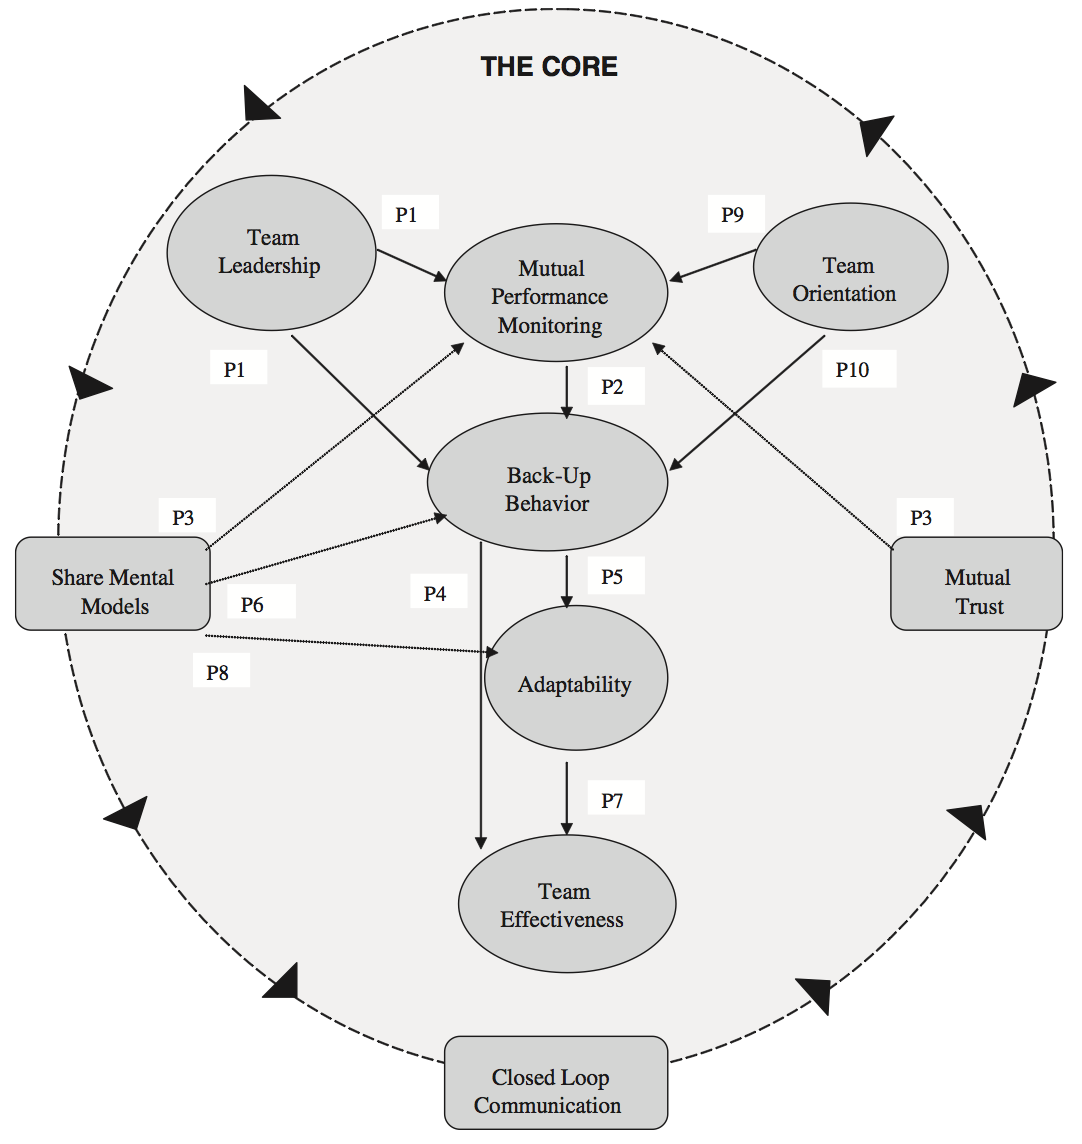
\includegraphics[width=150mm]{images/salas.png}
\caption{Graphical representation of the ``Big Five'' and supporting coordination mechanisms.}
\label{salas}
\end{figure}

There has been identified several impacts that trust can have on teams and team members. Bandow published a research on teamwork where she highlighted that trust affected several team processes and outcomes, e.g., membership contribution, team participation, product quality and cycle time. She further outlined that it is important that team members feel that their voice is heard, if not they will most likely be less willing to share their opinions and information. As a worst case scenario this might even lead to members not participating in information sharing arenas as they fear other members will perceive them as incompetent \cite{Bandow}. Also, without sufficient trust the team members might waste time and effort on checking each other as opposed to collaborating \cite{Cooper}. In general achieving mutual trust within projects seems to allow for information to flow more freely between the members. Without it there is a big chance it could spiral negatively and grow in concern where productivity goes down.

Similar findings to Salas et al. \cite{salas} were identified by Moe et al. \cite{moe} when they carried out a case study on a Scrum project. They state that ``without sufficient trust, team members will expend time and energy protecting, checking and inspecting each other as opposed to collaborating to provide value-added ideas. It is evident that trust is a prerequisite for shared leadership, feedback, and communication. Our finding regarding the lack of trust also confirms previous research on trust \cite{bandow}, such that team members may not be willing to share information if they fear being perceived as incompetent.". This highlights that trust is also identified as an important aspect in agile development.

Trust was also identified as a key factor both in small and large R\&D projects by Nygaard et al. \cite{}. They argue that small projects generally have a high level of trust because of the tight connections witnessed between partners and coordination benefits, while the larger projects usually benefit from having a high degree of variety in knowledge sources. They state that trust is a key factor for explaining exchange of knowledge and the creation of coordination benefits for organisations in most industries. They state that trust among partners supporting coordination and the aforementioned variety of knowledge flows within the projects is of uttermost importance to increase the likelihood of success. They back their work up by pointing to previous literature on similar research by McEvily et al. \cite{}.
\part{Research Methodology}
\chapter{Method}

\minitoc

The research study used different methods to gather the relevant publications that were selected. These are further outlined in this chapter starting with a detailed look at the literature review performed, as well as highlighting other parts of the gathering methodology, namely snowball sampling and general accumulation of papers.

\newpage

\section{Literature Review}

%Databases: Web of science (ISI), ACM, Science Direct (Elsevier), Google Scholar
%Keywords:
%Coordination, communication, collaboration
%Large-scale, multiteam, global
%Efficiency, Effectiveness, Productivity, Performance
%Location (co-located, collocated, colocated), distributed, dispersed
%Agile

For this study a literature review was chosen as the information gathering method. For the searching process and selection of articles in the literature review certain recommendations from systematic reviews were followed. The general procedure of such a review is outlined in L1 below. It is important to note that the searching had an open-mindedness regarding search words and the selection process.

\vspace{0.5cm}

\fbox{\parbox{\textwidth}{L1 - The steps of a systematic review \cite{khan2003}:
\begin{enumerate}
  \item Framing questions for a review.
  \item Identifying relevant work.
  \item Assessing the quality of studies.
  \item Summarizing the evidence.
  \item Interpreting the findings.
\end{enumerate}}}

\vspace{0.5cm}

Some of the benefits and objectives of a literature review are summarised in L2 below.

\vspace{0.5cm}

\fbox{\parbox{\textwidth}{L2 - Objectives of a literature review \cite{Oates2006}:
\begin{itemize}
  \item Show that the researcher is aware of existing work in the chosen topic area.
  \item Place the researcher's work in the context of what has already been published.
  \item Point to strengths, weaknesses, omissions or bias in the previous work.
  \item Identify key issues or crucial questions that are troubling the research community.
  \item Point to gaps that have not previously been identified or addressed by researchers.
  \item Identify theories that the researcher will test or explore by gathering data from the field.
  \item Suggest theories that might explain data the researcher has gathered from the field.
  \item Identify theories, genres, methods or algorithms that will be incorporated in the development of a computer application.
  \item Identify research methods or strategies that the researcher will use in the research.
  \item Enable subsequent researchers to understand the field and the researcher's work within that field.
\end{itemize}}}

\vspace{0.5cm}

\subsection{General Outline}

As explained in subsection \ref{general} a set of articles and publications were provided by the supervisor to give an overview on the field and agile software development in general. This made it easier to classify which studies to look for and how to evaluate their relevance and rigour. The databases used in the literature review are summarised in table \ref{databases}. When searching in these databases concepts and keywords were combined to match the research question as well as other interesting combinations. These concepts and keywords are outlined in table \ref{searchwords}. It is important to note that the last concept was an additional search word used because a lot of research seemed to either have focused on a co-located or a distributed manner.

\begin{table}[H]
\begin{center}
    \begin{tabular}{ | p{5cm} | p{8cm} |}
    \hline
    \textbf{Name} & \textbf{Impact} \\ \hline
    ISI Web of Science & apps.webofknowledge.com \\ \hline
    ACM Digital Library & dl.acm.org  \\ \hline
    Science Direct (Elsevier) & sciencedirect.com \\ \hline
    Google Scholar & scholar.google.com \\ \hline
    \end{tabular}
    \caption{Databases used in the literature review.}
    \label{databases}
\end{center}
\end{table}

\begin{table}[H]
\begin{center}
    \begin{tabular}{ | p{5cm} | p{8cm} |}
    \hline
    \textbf{Concept} & \textbf{Keywords} \\ \hline
    Coordination & Communication, collaboration \\ \hline
    Agile & Scrum, XP, Crystal, Lean, Kanban, Extreme Programming, Xtreme Programming  \\ \hline
    Large-scale & Global, multiteam/multi-team (systems), distributed, international \\ \hline
    Effectiveness & Efficiency, productivity, performance \\ \hline
    Location (Additional search words) & Co-located, collocated, colocated, co located, distributed, dispersed, global, globally, international  \\ \hline
    \end{tabular}
    \caption{Search words used in the literature review.}
    \label{searchwords}
\end{center}
\end{table}

The literature review provided an extensive amount of findings, unfortunately a lot of the publications were focusing on small-scale development. Therefore, a selection process had to be carried out. Here all abstracts of the collected literature were read and publications with the highest relevance were chosen. The articles that were still left after this selection process were then read thoroughly where some were discarded to give an appropriate amount of publications. The analysis outlined above focused mainly on finding articles focusing on large-scale agile inter-team coordination, meaning such articles were given a higher score when identified. Some other aspects that contributed to the score were mentioning of global projects, effectiveness and inter-team coordination in general. This process was important because of the time constraints specified on the study, and to obtain relevant and rigorous literature to insure a robust study.

\subsection{Snowball Sampling}

Snowball sampling is a term that reflects how new studies are selected through already chosen studies (based on their similarities) \cite{Goodman1961}. This was done in two ways in the research. In table \ref{databases} a list of databases used for the literature review are summarised. Some of these databases provided snowball sampling in the way of suggesting similar articles when a specific publication was selected from a search. This is the first way of snowballing used. The second way was through using reference lists in selected articles and publications. This extraction lead to a lot of well-written and recognised papers.

\subsection{General Accumulation}
\label{general}

Articles were also accumulated through a supervisor and fellow research students. At the start a handful of publications were received from the supervisor, and other papers were also acquired throughout the study. It is important to note that all the articles were inspected in the same manner as the publications found from the literature review to make sure their relevance and rigour were appropriate.

\section{Research Method}



\fbox{\parbox{\textwidth}{L3 -  TYPE OF CASE STUDY \cite{}:

}}

\subsection{Case Selection}
\label{case_selection}

Before the case study was conducted several criteria for a fitting case project were agreed upon. Seeing the research was suppose to focus on large-scale development/multiteam systems it was important to find a case where minimum two teams were present in the project, as well as collaborating across the teams. It was also important that the project performed in the case was an agile software development project. Another criteria was that the length of the project had to be suitable, meaning that the project had been ongoing for quite some time. The reasoning behind this was that the amount of data would be larger, and it would be easier to find patterns over a longer period of time.

There were also other criteria which were preferable, but not mandatory. One of these criteria was that it would be desirable if there were several roles within the project as a whole and the project teams. This had to do with the possibility of people with different roles within a project having various experiences from the course of the project leading to valuable data, or put in other words, having different points of view within the project. Another preferred criteria was having a large-scale project with several organisations involved. With several organisations involved there will be different cultures and protocols involved, and therefore a lot of interesting data could surface when comparing the approach of the different organisations.

\subsection{Data Collection}

For the data collection in the exploratory case study focus groups were selected. In these focus groups aspects that are known to be challenging in large-scale agile software development were brought up, as well as general discussion on the topic of large-scale software development. Focus groups are further outlined in L4, and were primarily selected because of their ability to accumulate extensive and valuable amounts of research data.

\fbox{\parbox{\textwidth}{L4 -  FOCUS GROUP \cite{}:

}}

In total three focus groups were conducted, one for each of the organisations involved. The topic that was looked at in the focus groups was ``Inter-team coordination and knowledge sharing''. The reasoning behind conducting focus groups for each of the organisations, and not performing them on a project level, was to make sure that an openness was achieved, and that data concerning specific organisations were not lost. As mentioned in section \ref{case_selection} there might be differences in cultures and methodologies between organisations, and these might not have been present in the focus groups if they were held on a joint basis.

The organisations were asked to provide their most relevant personnel to attend each focus group. In total 8 participants were involved in the focus groups. The participants had several roles in the Omega-project: development managers, scrum masters, (sub-)project managers, developers, delivery managers, functional architects and technical architects. It is important to note that most of the focus group participants were employees in management positions in the project. Most of these participants started as developers before switching to management roles with the course of the project. Because of the availability of personnel and topic in the focus groups no pure developers were present. The distribution of participants in the different focus groups is summarised in table \ref{pifg}.

\begin{table}[H]
\begin{center}
    \begin{tabular}{ | p{5.5cm} | p{4cm} | p{5cm} |}
    \hline
    \textbf{Theme} & \textbf{Organisation} & \textbf{Number of participants} \\ \hline
    \multirow{3}{*}{} & Alpha & 2 \\ \cline{2-3}
    Inter-team coordination and knowledge sharing & Beta & 3 \\ \cline{2-3}
    & Gamma & 3 \\ \hline
    \end{tabular}
    \caption{Participants in focus groups.}
    \label{pifg}
\end{center}
\end{table}

%TODO: Legg ved apendix til interview guides

Before the focus group sessions were conducted interview guides were developed, as well as a rough timeline of the project. The timeline was used to freshen the participants' memories about key events. In the focus groups the role of the researcher was to moderate the discussion and take notes. At the start of each focus group the participants were asked to explain their role(s) in the Omega-project. All of the focus group meetings were recorded digitally and transcribed at a later point in time, and whiteboard drawings were documented through pictures. In total the three focus groups resulted in 94 pages of transcribed material. Minutes of each focus group was also sent to each of the corresponding participants for needed information and review.

\subsection{Data Analysis}


\part{Results and Evaluation}
\chapter{Results}
\label{results}

\minitoc

In this chapter results from the case study will be highlighted. Starting of the chapter is an introduction and overview of the Omega-project, as well as a classification of the project in a multi-team system context. When this is performed the findings from all three focus groups are presented.


\newpage

\section{Clarification}

Before giving an overview of the Omega-project, both in a general fashion and in a multi-team system context, it is important to clarify that all quotations used in this chapter are translated from Norwegian to English by the researcher. The reason for this is because the focus groups and interviews carried out in the case study were conducted in Norwegian.

\section{Overview of the Omega-project}

To start of the result chapter it is important to get a clear overview of how the project was organised and conducted. The Omega-project was initiated and conducted by the public sector department Gamma. Gamma saw a need for a new office automation system, and especially argued that a new system was needed because the current platform was outdated and about to be abandoned. It is important to note that with the commencement of the Omega-project little was known about the content of the public reform, and therefore an agile development methodology and mindset was selected to take into account the high level of uncertainties and complex nature of the proposed project.

Omega is one of the largest IT development projects in Norway to date, consisting of approximately 175 members, where 100 of these came from five external companies. The project had a final budget of roughly 140 million euro. It lasted for about four years (January 2008 to March 2012) and had a strict deadline because of the reform. Around 800.000 person hours were used in developing {\raise.17ex\hbox{$\scriptstyle\mathtt{\sim}$}}300 epics with a total of {\raise.17ex\hbox{$\scriptstyle\mathtt{\sim}$}}2500 user stories. All of these were divided into 12 main releases (there were also smaller releases throughout the project). Figure \ref{releases} shows how these 12 releases where located in the timeline of the project.

\begin{figure}
\centering
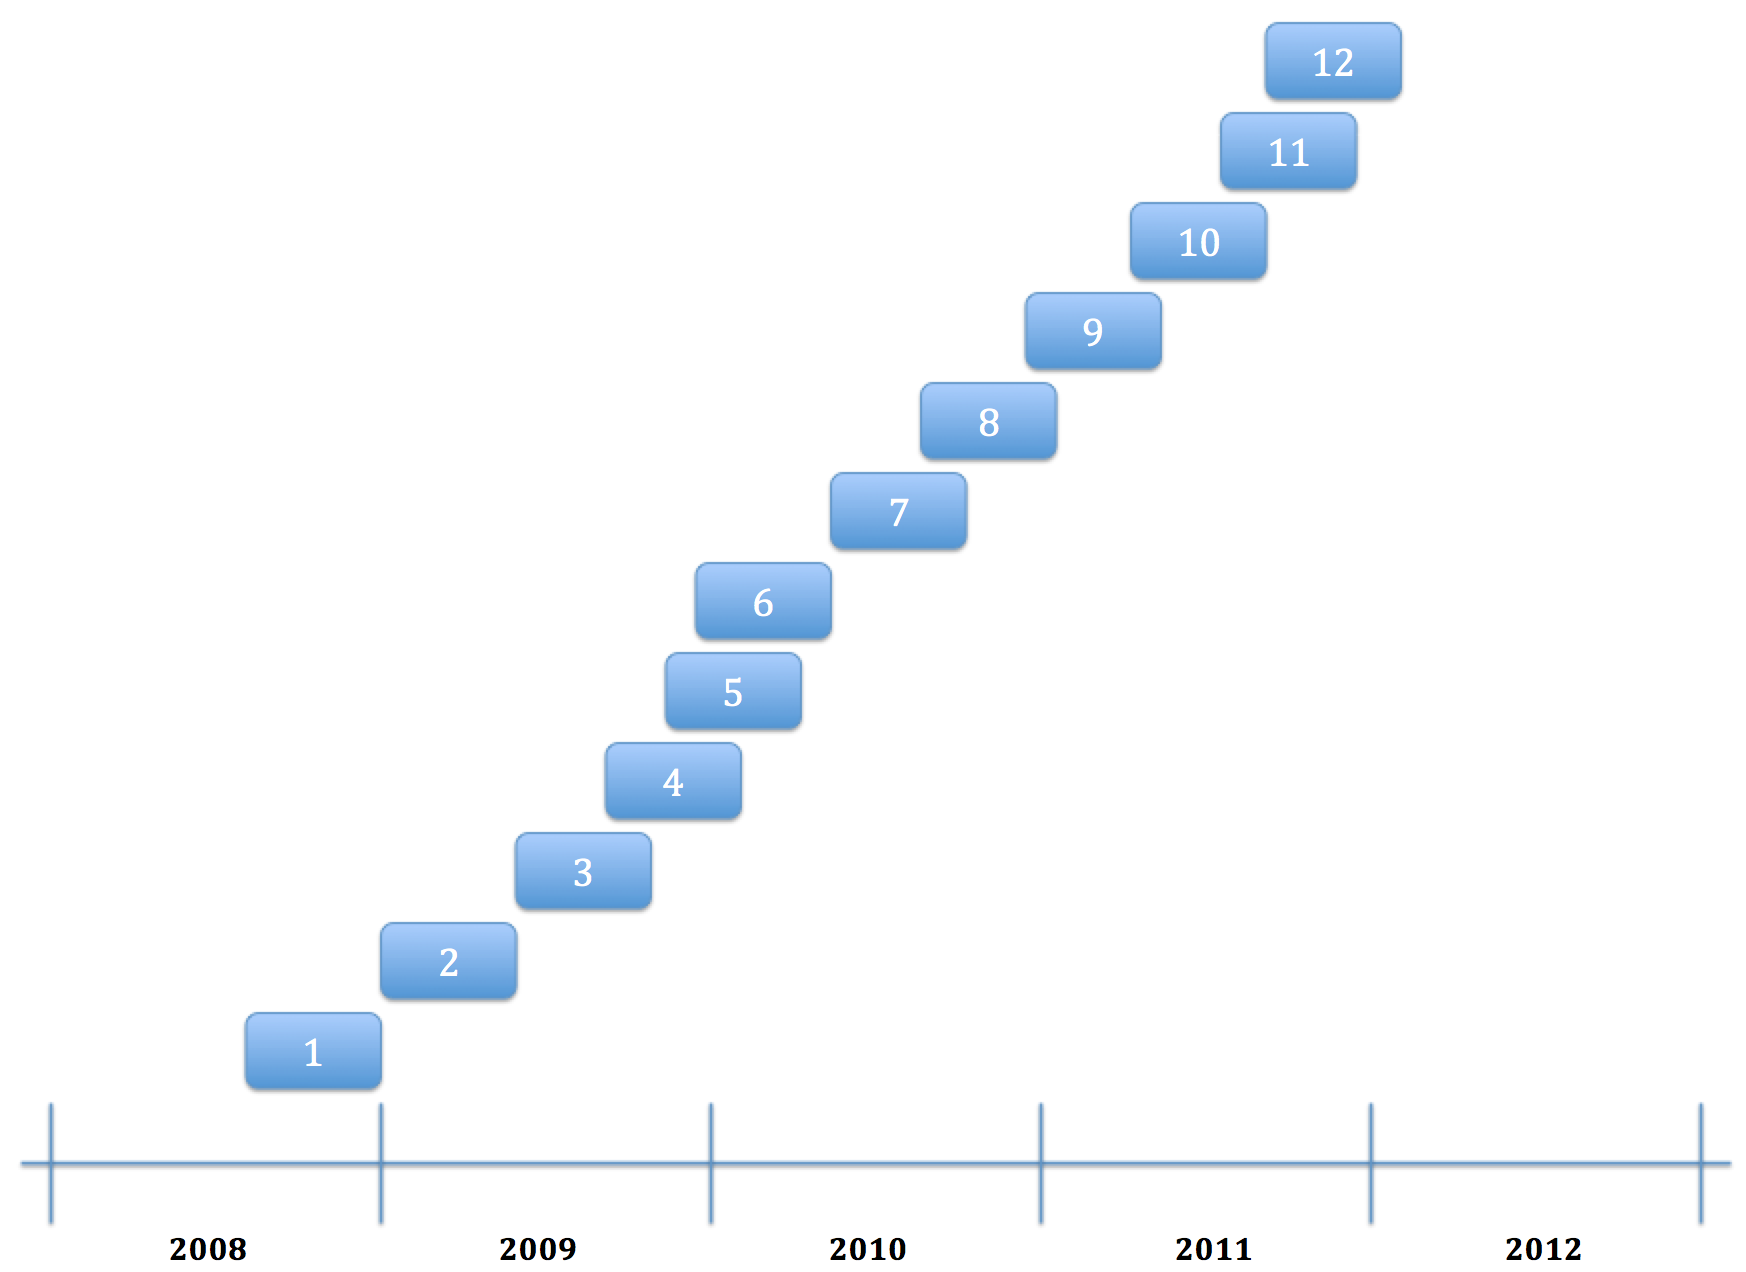
\includegraphics[trim = 0mm 0mm 0mm 0mm,width=155mm]{images/project_releases}
\caption{Main project releases in Omega.}
\label{releases}
\end{figure}

The initial project execution model consisted of six phases involving different personnel. The planned project execution was as follow: Starting of the project was a general requirements phase where potential impacts also were assessed. Here both business resources and architects were present. Following the general overview phase was a requirements analysis phase, again with both business and architecture resources. After these more general phases the solution description was worked on. The solution description was the main responsibility of the architecture unit, but business resources, developers, test resources and the heads of delivery were included. Going into the construction and approval phases all resources were collaborating to get continuous deliveries finished for production. In the production phase the main responsibility was put on the heads of delivery, but business and line resources were also present throughout the whole process, and architects, developers and testers were included in parts of the phase. The whole project execution model can be seen in figure \ref{project_execution}.

\begin{figure}
\centering
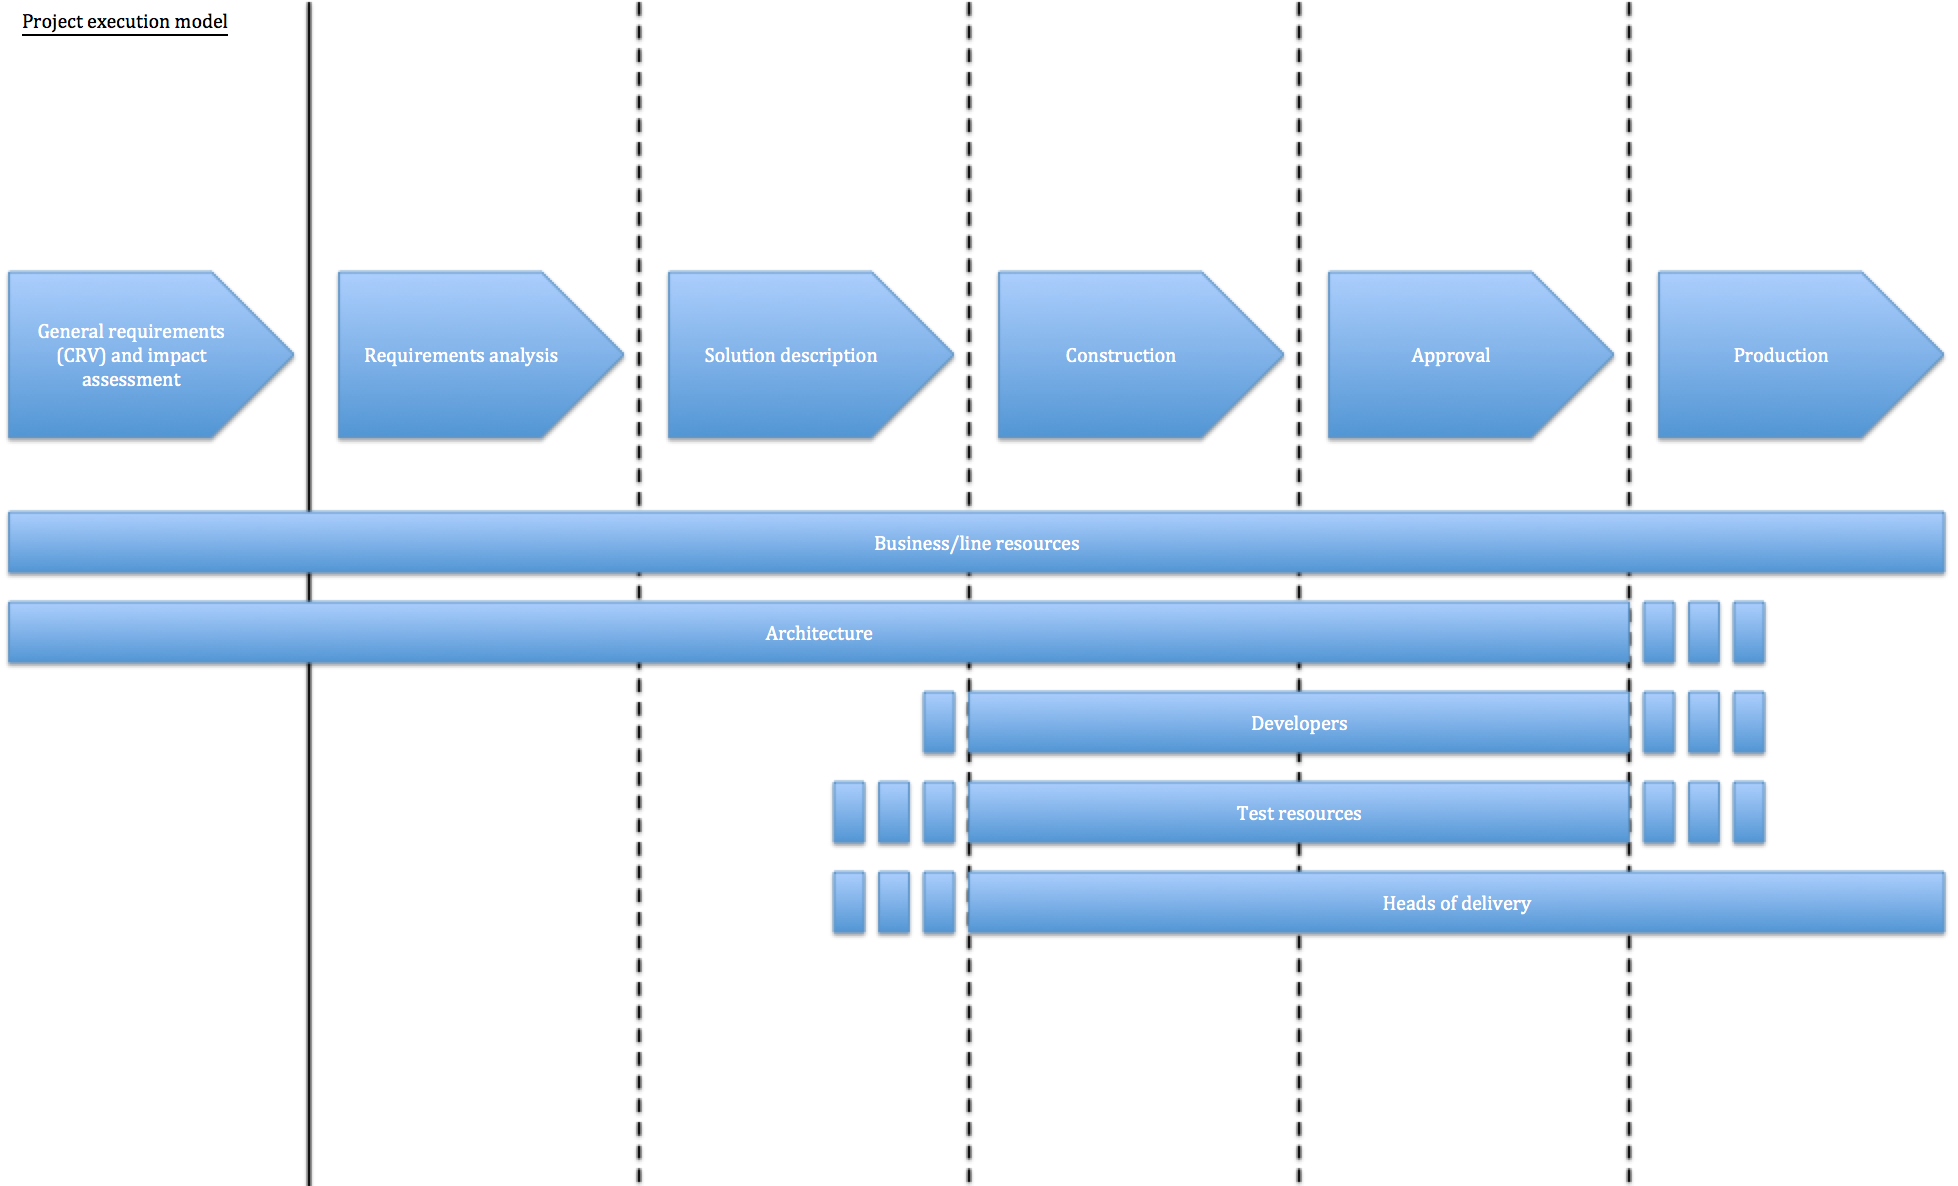
\includegraphics[trim = 0mm 0mm 0mm 0mm,width=155mm]{images/execution_model.png}
\caption{Project execution model.}
\label{project_execution}
\end{figure}

The project was organised with a ``project director'' at the top of the hierarchy mainly focusing on external relations. Underneath the project director there was a ``project manager'' responsible for operations. Omega also had four sub-projects with one ``sub-project manager'' each. These sub-projects were architecture, business, development and test, and are further described below. There were also a ``controller'' (or ``secretary'') present for administrative reasons. As can be seen from figure \ref{omega} the project used a matrix structure where the business and development sub-projects were both closely linked to the test and architecture sub-projects.

%TODO: Endre Alfa til Alpha
\begin{figure}
\centering
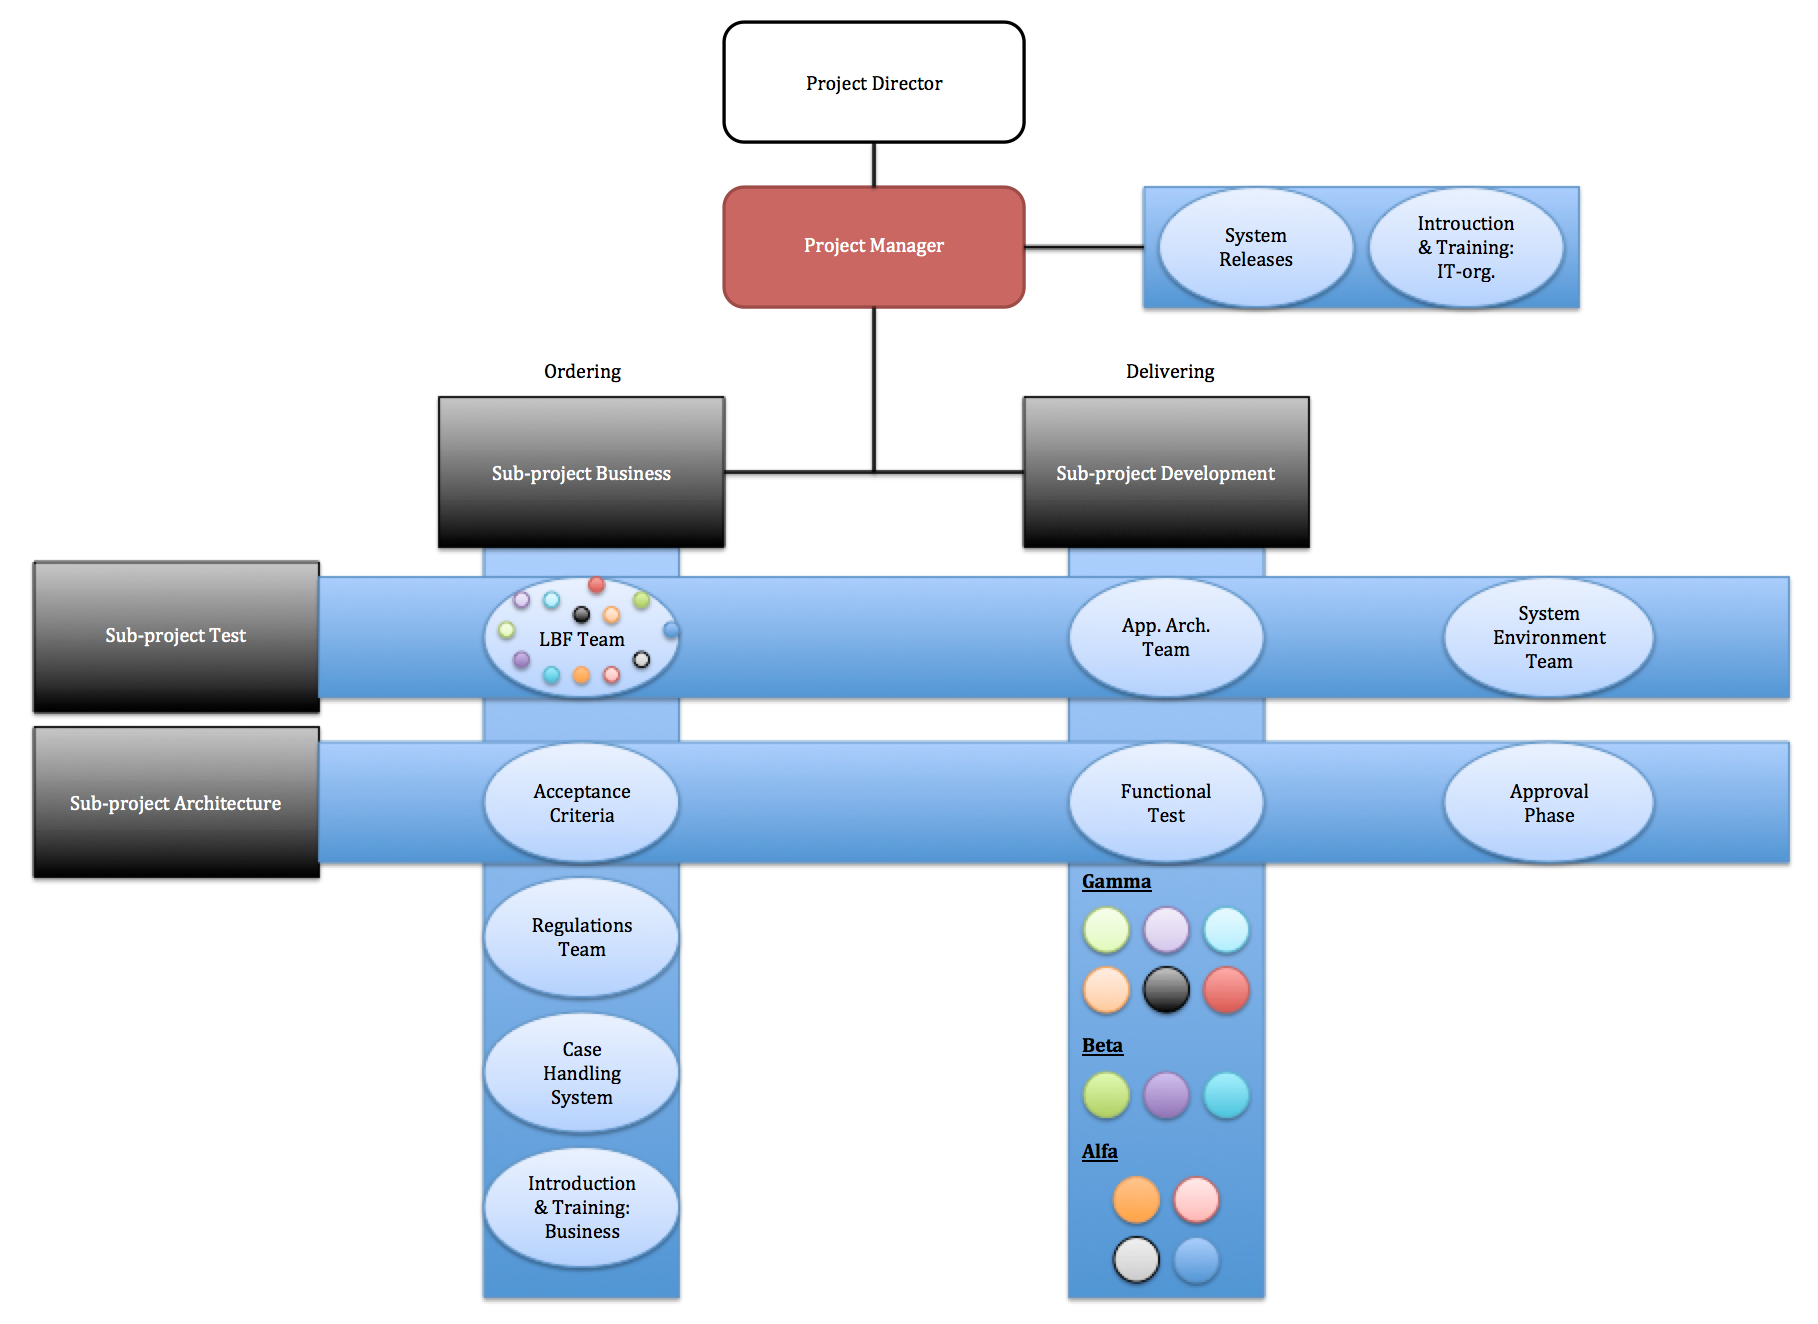
\includegraphics[trim = 0mm 0mm 0mm 0mm,width=155mm]{images/omega_organisation.png}
\caption{Omega-project's organisation.}
\label{omega}
\end{figure}

\begin{itemize}
   \item \textbf{Architecture:} Architects were in general responsible for the overall architecture of the project, but more specifically focused on solution description. They were also important in dealing with dependencies in Omega, and continuously updated a dependency map. The sub-project had head architects at a project management level and technical and functional architects located on a team level.
   \item \textbf{Business:} The business and line resources were present in the whole execution of the project (as can be seen from figure \ref{project_execution}). The responsibility of the business sub-project was to categorise needs and requirements, and then defining these into epics and user stories in a product backlog. In this sub-project there was a product owner team, but also other business and line resources (approximately 30 members at a peak period). Both functional and technical architects from the Scrum teams were also involved in the business sub-project.
   \item \textbf{Development:} The construction sub-project was further divided into three sub-projects led by Alpha, Beta and Gamma. The Gamma organisation had at most six development teams involved with both their own personnel and external consultants hired in from five different consulting companies. Alpha had at most four teams, while Beta had a maximum of three development teams. All 13 component teams worked corresponding to the Scrum methodology and delivered on a common demo day at the end of every three-week sprint iteration. There was also a system environment team present which was in charge of development and test environments. All roles of the Scrum teams are outlined in table \ref{trpist}.
   \item \textbf{Test:} The test sub-project had responsibility for all the testing of the project and the providing of deliverables from the development teams. Hence, they were important for quality assurance. The sub-project included a test leader, as well as test personnel from the development teams.
\end{itemize}

The main focus of this master thesis has been on the development of the system, and the personnel involved in this process. The development iterations had four phases: ``analysis of need'', ``solution description'', ``construction'' and ``approval''. These are further described below. The development process can be seen in figure \ref{initial_development_process}.

\begin{itemize}
   \item \textbf{Analysis of need:} Starting of each development release was an analysis phase. Here the focus was on functionality to be included in the coming release, and identifying and working out user stories. The product owner was involved in this process and was, e.g., responsible for prioritising the product backlog.
   \item \textbf{Solution description:} After identifying and working out general user stories in the ``analysis of need'' phase the user stories were further developed and made more comprehensive in the ``solution description'' phase. These user stories were also assigned to epics, and further estimated in approximate work-hours to completion before being assigned to different Scrum teams. Design and architectural choices were also determined in this phase.
   \item \textbf{Construction:} The construction phase typically consisted of five to seven sprint iterations per main development release. Here all development was carried out, and all work was functionally tested.
   \item \textbf{Approval:} In the last phase of each development release the delivered functionality was tested, both formal and non-formal functional testing was performed. This was done to assure both the internal and external interfaces were working as expected.
\end{itemize}

\begin{figure}[H]
\centering
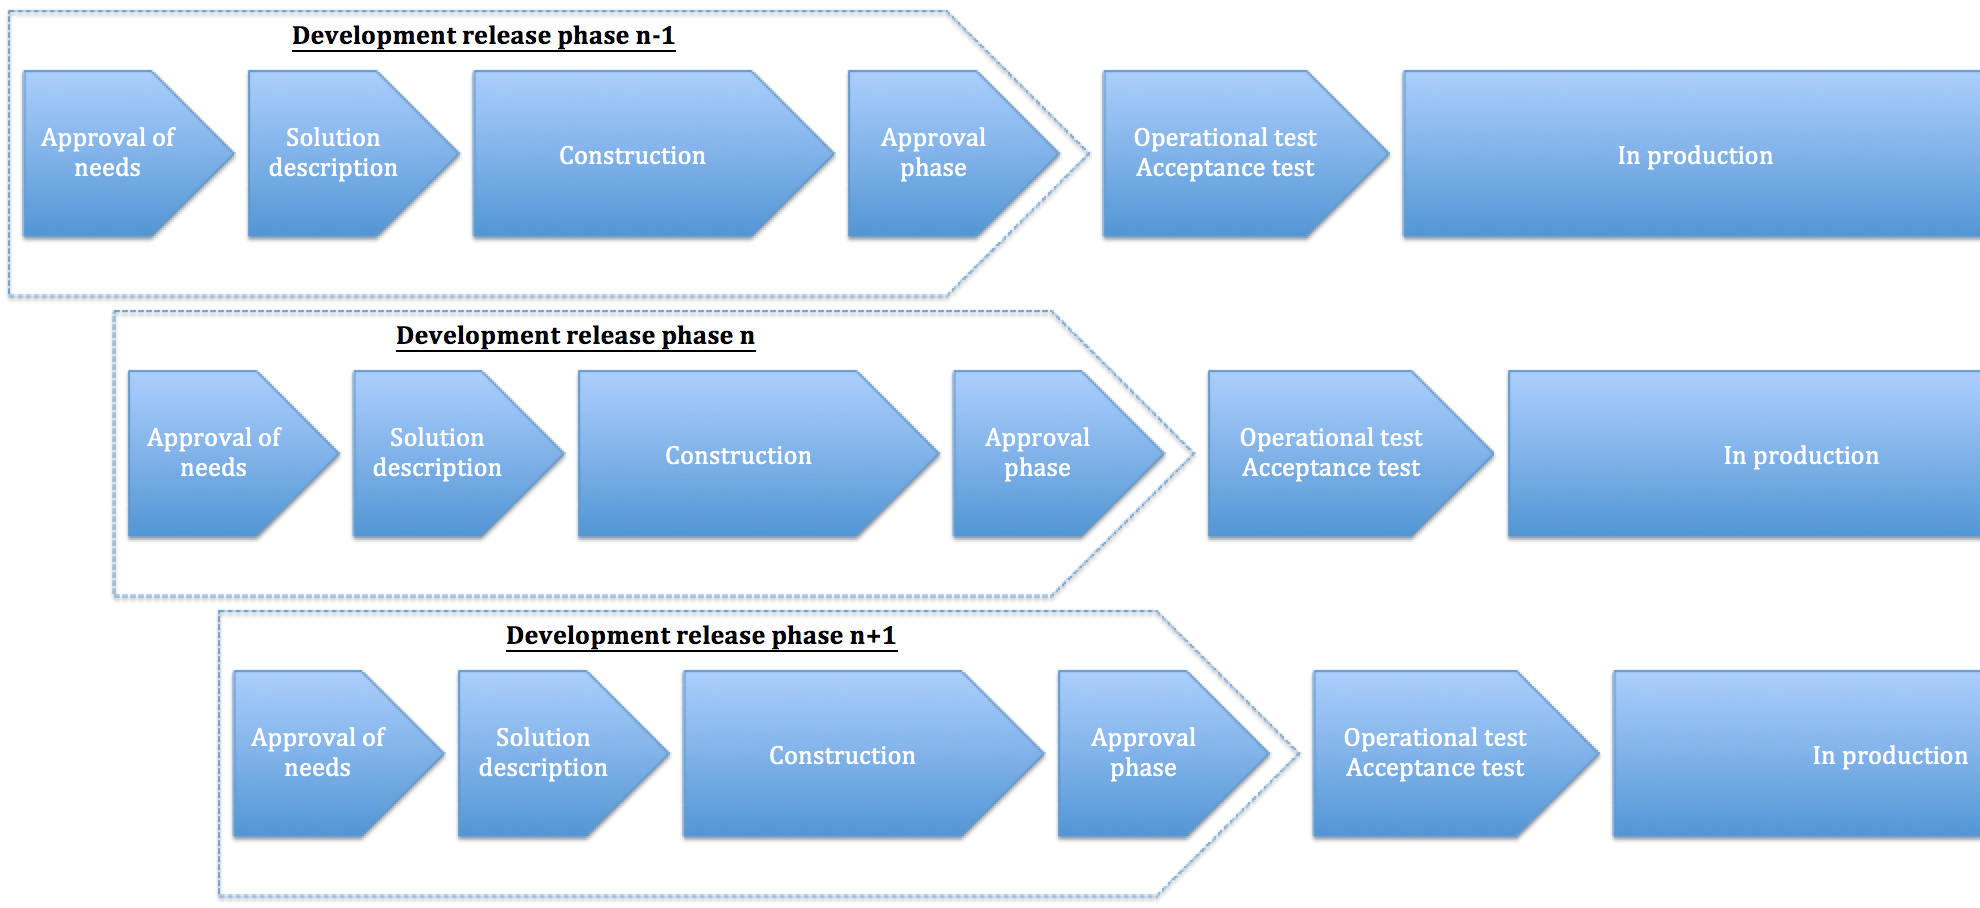
\includegraphics[trim = 0mm 0mm 0mm 0mm,width=155mm]{images/initial_development_process}
\caption{Initial development process.}
\label{initial_development_process}
\end{figure}

The development phase consisted primarily of several Scrum teams typically involving eight to nine members each. The roles in the different Scrum teams are further outlined in table \ref{trpist}. It is however important to remember that all members were somewhat cross-functional in the project. This means that a tester could for example have been 60\% tester, 30\% developer and 10\% designer, and a Scrum master could have been 50\% leader, 30\% architect and 20\% developer. 

\begin{center}
    \begin{longtable}{| p{4cm} | p{8cm} |}
   
    \hline \textbf{Role} & \textbf{Description of role} \\ \hline
    \endfirsthead

    \multicolumn{2}{c}%
{{\bfseries \tablename\ \thetable{} -- continued from previous page}} \\ \hline
    \textbf{Role} & \textbf{Description of role} \\ \hline
    \endhead

    \multicolumn{2}{|r|}{{Continued on the next page\ldots}} \\ \hline
    \endfoot

   \endlastfoot 

    Scrum master & The Scrum master facilitated all meetings such as the daily stand-up, demo presentations, retrospectives and iteration planning. Some teams rotated the role, while others had a fixed Scrum master. \\ \hline
    Functional architect & The functional architect was typically working 50\% with analysis and design, and 50\% as a developer. \\ \hline
    Technical architect & About half of the time went towards technical design, while the other half usually was spent developing. \\ \hline
    Tester & The person with the title ``tester'' was not responsible for doing all the testing, but was rather responsible for the tests being conducted. He was also in charge of writing and delivering test criteria to the sub-project test. The tests at the team level was unit tests, integration tests, system tests and system integration tests. Some of the teams did not have fixed testers, but rotated the role somewhat, e.g., at Beta. \\ \hline
    Developer & Each team had a mixture of four to five junior and senior developers. \\ \hline
    \caption{Team roles present in Scrum teams.}
    \label{trpist}
    \end{longtable}
\end{center}


\subsection{MTS Categorisation Overview}

To get a better overview and insight on how the project fits in a large-scale and MTS perspective a short description and classification is carried out. This is done through the use of multi-team system's three dimensions and their respective attributes, namely the ``compositional'', ``linkage'' and ``development'' dimension. For a description of each attribute please take a closer look at table \ref{domsc}. The overview of Omega is outlined in table \ref{ootopiamf}.

%Fiks tabell
\begin{center}
\begin{longtable}{ | p{2.5cm} | p{4cm} | p{8cm} | }

    \hline \textbf{Dimension} & \textbf{Attribute} & \textbf{} \\ \hline
    \endfirsthead

    \multicolumn{3}{c}%
{{\bfseries \tablename\ \thetable{} -- continued from previous page}} \\ \hline
   \textbf{Dimension} & \textbf{Attribute} & \textbf{} \\ \hline
    \endhead

    \multicolumn{3}{|r|}{{Continued on the next page\ldots}} \\ \hline
    \endfoot

   \endlastfoot 

	\multirow{10}{*}{Compositional} & Number & There was a maximum of 13 development teams at any given time (but also other teams involved such as project management) \\ \cline{2-3}
 	& Size & Approximately 175 members were involved in the MTS \\ \cline{2-3}
 	& Boundary status & The MTS is classified as an ``external MTS'', meaning there were more than one organisation involved in the project \\ \cline{2-3}
 	& Organisational diversity & There were in total five organisations taking part in the project, though three of these were the main organisations with the most members allocated to the project \\ \cline{2-3}
	& Proportional membership & Alpha had four development teams (31\%), Beta had three teams (23\%) and Gamma had six component teams (46\%) \\ \cline{2-3}
	& Functional diversity & Somewhat high degree of heterogeneity in core purposes and missions of the development teams \\ \cline{2-3}
	& Geographic dispersion & The teams were co-located in the same open-plan office space \\ \cline{2-3}
	& Cultural diversity & Low degree \\ \cline{2-3}
	& Motive structure & High degree \\ \cline{2-3}
	& Temporal orientation & High degree \\ \cline{2-3}
\hline
	\multirow{5}{*}{Linkage} & Interdependence & The degree of interdependence varied throughout the course of the project. The degree was also higher between certain teams compared to others, especially teams working on similar functionality \\ \cline{2-3}
 	& Hierarchical arrangement & Development teams were located at the same level in the hierarchical arrangement \\ \cline{2-3}
 	& Power distribution & The development teams had an even power distribution \\ \cline{2-3}
	& Communication structure: Network & Both informal and formal communication patterns were used \\ \cline{2-3}
	& Communication structure: Modality & Mainly face-to-face communication \\ \cline{2-3}
\hline
	\multirow{6}{*}{Developmental} & Genesis & Appointed \\ \cline{2-3}
 	& Direction of development & Became a formalised MTS, but now finished \\ \cline{2-3}
	& Tenure & Approximately four years \\ \cline{2-3}
	& Stage & Finished \\ \cline{2-3}
	& Transformation of system composition: Membership constancy & Some fluidity depending on need throughout the Omega-project \\ \cline{2-3}
	& Transformation of system composition: Linkage constancy & Some communication lines and arenas were fluid, changing base on a need basis, while others were constant through the whole project \\ \cline{2-3}
	\hline
\caption{Overview of the Omega-project in a MTS fashion}
\label{ootopiamf}
\end{longtable}
\end{center}

\section{Coordination Arenas and Important Aspects}

After the transcription and coding of the three interviews it was soon established that the amount of coordination arenas carried out throughout the course of the Omega-project was extensive. The different coordination arenas and mechanisms witnessed in the project were both performed across the three organisations (Alpha, Beta and Gamma), and across teams within each of the specific organisations. These coordination mechanisms are summarised in three tables. Table \ref{cmuatwo} summarises all the coordination mechanisms identified across the boundaries of the organisations. Table \ref{cmuasito} outlines different coordination methods used within the different organisations to achieve coordination, collaboration and communication across their respective teams. While table \ref{ocmaia} describes several other mechanisms and aspects which were deemed important in the success of the project.

Considering the sheer amount of coordination mechanisms and other important aspect it was necessary to decide which ones to prosecute further. After reading through both the transcribed interviews and the coding numerous times some mechanisms and aspects seemed to surface in several of the interviews. The main themes identified were these five elements which will be investigated and described further in the coming sections (it is important to note that some of these might overlap to some degree, e.g., co-location and the use of informal communication arenas):

\begin{itemize}
   \item Co-location
   \item Informal communication arenas
   \item Continuous change and improvement
   \item Presence from project management and owner
   \item Mutual trust and shared mental models
\end{itemize}

%\begin{table}[H]
\begin{center}
    \begin{longtable}{| p{6cm} | p{9cm} |}

    \hline \textbf{Coordination mechanism} & \textbf{Description of mechanism} \\ \hline
    \endfirsthead

    \multicolumn{2}{c}%
{{\bfseries \tablename\ \thetable{} -- continued from previous page}} \\ \hline
    \textbf{Coordination mechanism} & \textbf{Description of mechanism} \\ \hline
    \endhead

    \multicolumn{2}{|r|}{{Continued on the next page\ldots}} \\ \hline
    \endfoot

   \endlastfoot

    Metascrum & A meeting similar to Scrum of Scrums but with less details which was held twice per week. Attending the metascrum was the project leaders and all the sub-project leaders from test, architecture, business and development. A ``technical metascrum'' was tested, but was shortly shut down after initiation. \\ \hline
    Planning day & The planning day was a form of kick-off for each sprint iteration where the project members met up with the project owner. The planning day was performed on three levels: project, organisation (Alpha, Beta and Gamma) and team. A rough sketch of the focus areas and work to be performed in the coming sprint was presented with a distribution towards each of the three organisations by the project owner. After this the organisations distributed the work on their respective teams, and lastly the teams got together separately and worked out a contract with estimated work to be performed which was delivered to the project owner team. Before the planning day commenced the developers also had a ``developer forum'' where development-oriented information and discussion was carried out. This was however held on an organisation basis, and not across the three organisations. \\ \hline
    Demo & Demo presentations were held by all Scrum teams at the end of each sprint iteration where everyone could attend. Each team was allocated approximately 10 minutes. There were also larger demo presentations for the project owner when a new release was finished. Some teams in addition started performing smaller demo sessions within the iterations to get rapid feedback. \\ \hline
    Pre-planning day & Before the ``planning day'' was carried out a pre-planning day was performed. Here typically different types of architects (especially functional architects) and the project owner (as well as some other members of the project owner's team) met to create a rough classification and allocation of work to the different Scrum teams for the coming sprint iteration. The allocated work was listed in a prioritised manner. \\ \hline
    Dependency meeting & A meeting held between all Scrum masters from the Alpha, Beta and Gamma teams. This meeting was held on the ``Planning day'' where the focus was on discovering dependencies across Scrum teams. However, these meetings faded away early on because of the dependencies being discovered and handled elsewhere. \\ \hline
    Solution description / ``Master plan'' & At the start of the Omega-project a larger solution description phase was performed involving a lot of architects (as can be seen from figure \ref{project_execution}). This lead to a ``master plan'' for the project and was documented in an issue tracker program called Jira. The ``master plan'' was continuously altered throughout the course of the development phase as outlined in figure \ref{initial_development_process}. In the solution description meetings important aspects were discussed such as coordination across organisations and management of activities. An example of what came out of these meetings was a dependency map of the whole Omega-project, which was in constant change. Part of the solution description meetings were also negotiation and estimation meetings which were important for the contract for each release. \\ \hline
    Jira and Wiki/Confluence & Different programs and forums were used for documentation and tracking within the project. In Jira all user stories and epics were located, and different information about the project and current sprint iteration could be seen on different levels, such as project and team level. The dependency map for the whole Omega-project was also located in Jira. Confluence was the main program used as a wiki. Here solution descriptions, team routines, routines across teams, system documentation, check lists, retrospectives, architectural guidelines, functional test etc. were all located. \\ \hline
    Open-space & An arena held on a voluntary and need basis, which was used for exchanging experiences. It was however only used during a few of the releases. Participants suggested the topics beforehand, leading to agendas for the open-space sessions. \\ \hline
    Jabber & Jabber was introduced as an instant messaging service in the Omega-project after being identified as something needed in one of the Open-space sessions. Here project members could ask both formal questions, e.g., technical questions, and informal questions or activities, e.g., wine lotteries. \\ \hline
    Lunch seminars & Lunch seminars were kind of similar to the ``open-space'' sessions. Typically two to three topics were held by project-personnel on relevant and interesting topics, often regarding themes correlated to the current situation of the project. As with the ``open-space'' session these seminars were also held on a certain period of the project before fading away. \\ \hline
    Front-end meeting & The front-end developers worked with a complex framework called Flex. Because of this a lot of coordination had to be handled between teams working with this framework from all organisations. Therefore, front-end meetings were held, were typically the most prominent Flex-developers happened to be present. \\ \hline
    Technical architecture forum & At the technical architecture forum all technical architects met up to discuss what was to be done in the coding base to prevent coordination issues. These meetings were slowly fading away because the need was covered in other arenas. \\ \hline
    Architecture council & At these gatherings an architecture council listened to all team architects present their respective team's tasks for each sprint iteration. \\ \hline
    Business meeting & The business part of the Omega-project was coordinated through meetings where the business architects from Alpha, Beta and Gamma met up with the business unit from the project owner. Here the sprint iteration queue, and the current status of the project and sprint was presented. This meeting was held around one time each week or every other week. \\ \hline
    Bug-board discussion & The quality assurance unit with its testers had frequent meetings around bug-boards, especially after new releases and around acceptance testing. In the period after a new release these meetings were often held on a daily basis. Here all the bugs were gone through and allocated to the responsible Scrum team in either Alpha, Beta or Gamma. \\ \hline
    
    \caption{Coordination mechanisms used across the whole Omega-project.}
    \label{cmuatwo} 
    \end{longtable}
\end{center}
%\end{table}

\begin{center}
    \begin{longtable}{| p{6cm} | p{9cm} |}

    \hline \textbf{Coordination mechanism} & \textbf{Description of mechanism} \\ \hline
    \endfirsthead

    \multicolumn{2}{c}%
{{\bfseries \tablename\ \thetable{} -- continued from previous page}} \\ \hline
    \textbf{Coordination mechanism} & \textbf{Description of mechanism} \\ \hline
    \endhead

    \multicolumn{2}{|r|}{{Continued on the next page\ldots}} \\ \hline
    \endfoot

   \endlastfoot

    Scrum of Scrums (SoS) & Scrum of Scrums were meetings held by all organisations (Alpha, Beta and Gamma) ranging from two to three times per week. In these meetings all Scrum masters from the corresponding organisation, as well as project management (project leader, test leader, head technical architect, head functional architect, business leader and development leader). The main goal of the SoSs was to identify and handle obstacles. There were also held a few SoS meetings across organisations to handle potential changes to the contracts. \\ \hline
    Technical corner & The ``technical corner'' was a meeting Beta had in an early stage of the project. It was held on Fridays for about 1-1,5 hour. Here team architects presented important themes for the Beta-members. After a while it was shut down because of lack of interest and topics. \\ \hline
    Experience forum & The experience forum was an arena established in the Alpha-organisation for exchanging experiences. Here Scrum masters and the development manager met to discuss topics such as retrospectives, the planning day, and how work was performed by the Alpha-organisation's Scrum teams. It could be seen as a coaching-session with exchange of ideas and thoughts. \\ \hline
    Retrospective & Retrospectives were used on several levels in the project. All of the organisations used it on a pure Scrum team level, but some also used it on both the solution description personnel and in the project management team. The retrospectives for each Scrum team were held after the demo on Fridays. Here negative and positive information and aspects were brought forward and documented in Confluence. A few ``global retrospectives'' were also tested but swiftly faded away. \\ \hline
    Technical and functional architecture meetings & Both technical and functional architects had separate meetings within the different organisations. These meetings were typically short and held on a weekly or biweekly basis. The meetings were as mentioned brief and were primarily used for status updates, and keeping the technical and functional managers up-to-date to make the cross-coordination meetings with the other organisations easier and more precise. \\ \hline
    Supplier meeting & At Alpha a supplier meeting was held by the project leader for all Alpha-members. The project leader contributed with practical information regarding the project. In these meetings different members held presentation on different topics such as clean code, test driven development and project guidelines to keep the technical level of the personnel up to scratch. \\ \hline
    Meeting about queue & Alpha also had a meeting regarding ``what was next in the queue?'', ``what is the next delivery?'', ``what is the status on current user stories?'' and ``what is it that we feel is needed to drive the queue forward?''. These meetings were held with the functional architect, development manager and product owner from Gamma. \\ \hline

    \caption{Coordination mechanisms used across teams within the specific organisations (Alpha, Beta and Gamma) in the Omega-project.}
    \label{cmuasito}
    \end{longtable}
\end{center}

\begin{center}
    \begin{longtable}{| p{6cm} | p{9cm} |}
   
    \hline \textbf{Mechanism/Aspect} & \textbf{Description} \\ \hline
    \endfirsthead

    \multicolumn{2}{c}%
{{\bfseries \tablename\ \thetable{} -- continued from previous page}} \\ \hline
    \textbf{Mechanism/Aspect} & \textbf{Description} \\ \hline
    \endhead

    \multicolumn{2}{|r|}{{Continued on the next page\ldots}} \\ \hline
    \endfoot

   \endlastfoot 

    Stand-up & Daily stand-ups were used on all Scrum teams in the project. Here obstacles, progression and possible needs were voiced around the Scrum-boards. Introduced by Gamma was also the way of organising the stand-up meeting such that they were held on different timeslots. This made it possible for members to attend several stand-ups if necessary. \\ \hline
    Board discussion & An important aspect for coordination, discussion and status updates in the project was the frequent use of whiteboards. The stand-up meetings were for instance held around these boards, and on these boards the workload for each sprint iteration was put up and updated as the sprint moved along. The backside of the boards were left open to carry out informal discussion when needed. \\ \hline
    Co-location & One of the biggest impacts on the project, and coordination, collaboration and communication within the project was the radical co-location. This co-location came at an early stage (with the introduction of Alpha and Beta) in the project where all teams, as well as project management, were located in an open-plan office space at the same floor. \\ \hline
    Project management in same location & In both Alpha and Beta management by ``walking around, talking around'' was brought up. Because the project management was located in the same office space as the other project teams it was easy for them to keep track and manage by just being present. With management being close by it was, e.g., possible for development managers to have informal communication with each Scrum master every day, making sure they were up-to-date on the progress. This lead to easier decision making and problem handling for the project management team. Another important and positive factor was that decision making could be taken rapidly through more informal arenas, as teams could address project management at once without having to book formal meetings every time a decision had to be made. \\ \hline
    Informal communication & Another important impact on the coordination and general information sharing was the extensive use of informal communication. These communication arenas seemed to be very important in the agile mindset because of the pressure to deliver within a short period of time. With the use of informal communication arenas decisions could be made faster than using formal arenas such as having to book meetings where, e.g., timeslots had to match for participants. As the project progressed the informal communication arenas were more and more present, often replacing some of the formal communication arenas. \\ \hline
    Joint coffee break & An informal communication arena that was present throughout the Omega-project was the ongoing discussion around the coffee machine area. There were even joint coffee breaks at 2PM every day. These informal meetings saw a growth as the project moved along. \\ \hline
    Pair programming & Pair programming was introduced by Beta and adopted by some of the other organisations. Often the pairs consisted of one senior and one junior developer. The main reasons for using pair programming was to achieve a higher standard on the coding, increase knowledge (especially of junior developers) and to build better relationships and trust within teams. Pair programming was also tested across teams, but was not deemed successful. \\ \hline
    Trust & Another important aspect of the project was trust, both within and across organisations, but also between the organisations (Alpha, Beta and Gamma) and the product owner. Trust was increased through several ways, e.g., social gatherings, co-location and a general openness culture. With the increase in trust between the different project-members there was an increase in informal communication arenas, and a decrease in formal ones, leading to more rapid decision making, in line with the agile mindset. \\ \hline
    Rotation of team members & At Beta some rotation of members across the Scrum teams happened. This was mainly to spread competence and knowledge across teams to make them more ``all round teams'' able to handle different types of work. There were also a few rotations because of personal chemistry. \\ \hline
    Rotation of team placement & Another decision made by Beta and Gamma was to change location within the office space of some teams. This was a deliberate move by the project management to achieve better collaboration and communication, especially on the informal level, between teams working on similar parts of the project. \\ \hline
    Alpha/Beta-personnel placed in Gamma teams & An aspect that might have been important both for trust and the informal communication was that both Alpha and Beta members were located in Gamma teams. This probably made it easier to get informal communication going at an early stage of the Omega-project because some members knew each other across the organisations and teams already. \\ \hline
    Continuous planning and change & Self-organising was present at different levels in Omega such as team, organisation and project level. At the team level the teams changed their ways as the project moved along introducing new and removing old aspects, e.g., moving from pair programming to individual programming when knowledge increased. At both the organisational level and the project level different communication arenas were changed on a need-basis. This had mainly to do with the respective arenas being covered elsewhere, e.g., through informal communication. Another part of the project where continuous planning and change was present was within the dependency mapping and solution description. \\ \hline
    3-level hierarchy from product owner & Mentioned by Gamma was the way the product owner was organised within the project. At the top of the food change the main product owner sat, then three representatives from the product owner were located at Alpha, Beta and Gamma, and at the bottom of the hierarchy the product owner had functional experts and architects inside or close to the teams. This led to easier decision making as the representatives further down the hierarchy could answer on the behalf of the product owner, or at least knew who to ask for the answer increasing the pace of development and problem solving. \\ \hline

    \caption{Other coordination mechanisms and important aspects.}
    \label{ocmaia}
    \end{longtable}
\end{center}

\subsection{Co-location}

After the introduction of Alpha and Beta into the Omega-project in 2009 it was decided that all the development teams (as well as project management teams attached to the project) were to be co-located in a single-floor open office space. In all of the interviews conducted this was something that was brought up as an important factor for achieving a high level of efficient coordination within the project. Some quotations are included from one of the project leaders at Alpha to give a brief overview of his thoughts:

\begin{fancyquotes}
But also sitting in the same landscape [was important], when you, e.g., can see that a team has been drawing on the board for two hours, then it is time to head over and check what is going on, and if you can contribute. [...] So I think being located on the same floor was an important factor. It is something I have noticed at Zeta [another large-scale development project], not being located at the same floor, it is a lot more difficult to keep track of what is going on. 
\end{fancyquotes}

This project leader further explained the importance of being co-located in the project, and how this could be an aspect hard to replicate in other large-scale projects because of the sheer amount of personnel and size connected to such development:

\begin{fancyquotes}
It is easy to recreate metascrums, Scrum of Scrums and the experience and knowledge sharing. The concrete, specific aspects are easy to replicate, but the team dynamics, \textbf{having everyone located at the same floor}, constant communication, the togetherness witnessed, and similar things, the less concrete aspects, they are harder to reproduce.
\end{fancyquotes}

The views regarding co-location identified in the Alpha-interview was also shared by interviewees from the other interviews. An architect from Beta described an example of two teams located in the building next-door, where this small distance already caused problems for communication and general collaboration:

\begin{fancyquotes}
I for instance talked to a management team located with an environment team in the building next-door, and they rarely experienced visitors from other units of the project. So having to walk up one stair [which was one meter long], as well as opening and closing two doors seemed to be enough [to hinder communication].
\end{fancyquotes}

Another project leader, now from Beta, also added his thoughts on the impact of co-location on communication, collaboration and coordination which nicely sums up the general view of the interviewees:

\begin{fancyquotes}
I think being co-located was a big advantage, especially having all the teams located on the same floor and space. If you are, e.g., located at each side of a town or building it would be a barrier for communication.
\end{fancyquotes}

\subsection{Informal Communication Arenas}

An aspect that was identified several times throughout the different interviews was the mentioning of ``informal communication arenas''. Several of the interviewees seemed to suggest that the informal communication witnessed in the project was one of the reasons behind achieving a higher degree of efficiency in the everyday work. In the interview with Gamma one of the project leaders from the organisation noted that the high degree of verbal face-to-face communication internally in the project was important. It was especially three arenas that were mentioned numerous times (outside of the general day-to-day conversations and communication): shared lunches, fixed joint coffee breaks, and the extensive use of whiteboards.

What was also mentioned as an enabler for the high level of informal communication arenas was the aforementioned co-location of the project teams. A Scrum master from Gamma noted:

\begin{fancyquotes}
With short distance to the other teams it was easy to make decisions orally and upfront, and we avoided misunderstandings that could have occurred with having to write everything down on paper, sending e-mails and similar stuff. You could handle everything upfront.
\end{fancyquotes}

A functional architect from Beta also had similar thoughts on the matter of informal versus formal meetings on the spot. As can be seen from the quotation below he felt that it was easier to just handle the needed discussion then and there without having to go through formal arenas, such as booking meeting-rooms which were located on another floor. Again this shows the impact of co-location on the increased use of informal communication arenas:

\begin{fancyquotes}
When spontaneous need for discussion emerged, the need to walk up a few floors or having to book a meeting-room or similar, it was just too cumbersome.
\end{fancyquotes}

Another aspect that was mentioned as a possible support for the informal communication arenas was having consultants from both Alpha and Beta located in Gamma-teams. This was both noted in the interview with Beta and Gamma. An architect from Gamma had the following to say on the matter:

\begin{fancyquotes}
But there were quite a few Alpha- and Beta-consultants in the Gamma-teams. So there were always several members knowing each other across the teams and organisations, meaning the informal channels were definitely present.
\end{fancyquotes}

Not only was the use of informal communication present from an early stage of Omega, it also seemed to be increasing throughout the project. Quite a few of the interviewees highlighted the increasing use of whiteboards, joint coffee breaks and common lunches. There was even introduced an internal system called ``Jabber'' where project members could ask anything, e.g., technical questions or arranging wine lotteries. An architect from Beta suggested that the use of formal arenas seemed to be of a higher importance in the earlier stages of the project, but decreased after a while when people knew who to contact for different inquiries:

\begin{fancyquotes}
I imagine that the need for such [formal] meeting-places are important in the start, but less important as the members get to know each other. You get more comfortable with just approaching the person you know can fix the issue.
\end{fancyquotes}

The most important aspect of the use of informal communication seemed to be that things got handled instantly, and were not left alone, or postponed to the formal meetings. One of the project leaders at Alpha tried to describe how this was important to achieve an agile way of developing and working:

\begin{fancyquotes}
What is important in agile [development]? You need to deliver within three weeks. Then you don't have the time to wait for someone to read through all his e-mails before he answers yours after two weeks of waiting. You should rather just approach the person and ask for a few minutes of his time. You might even get the answer in ten seconds, but having to open and read an e-mail is time-consuming. But it is important to not overdo it [the informal communication] either, because this could lead to disturbances in the workplace. There is always a balance [between formal and informal communication].
\end{fancyquotes}

An architect at Beta further outlined this aspect of informal communication describing how these arenas in turn made the formal arenas less complex and time-consuming because, e.g., dependence issues were already dealt with and did not have to be handled in the formal meetings:

\begin{fancyquotes}
I think there were few [dependencies], because the teams did not wait for the Scrum of Scrums, they handled it then and there. [...] I felt that the informal channels worked better than trying to arrange formal meetings where things were discussed [e.g., dependencies].
\end{fancyquotes}

Some side effects were also spawned with these informal arenas. Something that was witnessed as a response to the increasing use of informal communication across and within the teams was the use of earplugs or headsets. As a project manager at Alpha described it:

\begin{fancyquotes}
If you saw someone wearing a headset you instantly became more restrictive towards approaching and talking to that person.
\end{fancyquotes}

Even though the informal communication arenas seemed to be more and more present throughout the course of the project some interviewees highlighted that there has to be a balance between the informal and formal channels, and that a project will not function efficiently without both being existent. As a project leader from Beta put it:

\begin{fancyquotes}
I think you need both [informal and formal arenas], but without the informal communication and the common determination to work things out, then I don't think large-scale projects will work. However, I don't think you can manage to control such a project well enough with only formal channels.
\end{fancyquotes}

\subsection{Continuous Change and Improvement}

A third aspect that was identified as being important for the project was how everything was continuously improving through change, especially coordination arenas. When it was identified that an arena had ceased to serve its purpose it was shutdown. The decision to stop or start using a particular meeting or arena was typically decided in the metascrum-meetings as one of the project leaders at Gamma put it:

\begin{fancyquotes}
We adjusted which meetings were used on a need basis within the project. Some arenas were present throughout the whole project, while other came and went. I believe this was important. [...] E.g., we could identify in a metascrum-meeting that there were areas which needed more, or less, coordination.
\end{fancyquotes}

As mentioned in the previous section on ``informal communication arenas'' there seemed to be a growing use of informal channels, e.g., more use of whiteboards, and more joint coffee breaks and lunches. A project leader at Alpha argued that the efficiency and production level evolved with the small continuous changes and improvements, but admitted that this was probably hard to measure:

\begin{fancyquotes}
What would have been interesting to see if we had proper story-points was the actual growth in story-points delivered. Unfortunately these story-points were bound to hours, so it is not possible to say that we were way better at the end compared to the beginning, even though we definitely were. And I believe this was because of all the small changes we made. Some large, but mainly the small continuously improvements which were performed on all levels.
\end{fancyquotes}

The same project leader further added to this discussion. He felt that being able to actually set aside time for knowledge sharing and general thoughts was an important aspect of the continuous improvement, mentioning retrospectives as one of the factors:

\begin{fancyquotes}
The first delivery was somewhat a ``try-and-fail'' process. When the second delivery came along we had had done it before, and some of the stuff was standardised. And then we had continuous improvement throughout. We were even allowed to set aside time for this. Often people do not think about using retrospectives.
\end{fancyquotes}

The continuous change and improvement was not only identified in the changing of which meetings were in use, but also in other areas of the project. A project leader at Beta mentioned how the teams were self-organising, as well as how they decided to rotate some of the teams and team members to achieve more generalised component teams:

\begin{fancyquotes}
Self-organisation was a reoccurring thing. E.g., you could not force a self-organising team to do pair programming strictly throughout the whole project, but could have it as a principle, and then let the team decide when it was not needed anymore. [...] But after a while we identified the need of spreading the knowledge and competence, to go from specialised teams to more general teams. From specialists to all-rounders.
\end{fancyquotes}

Especially the architectural side of the project seemed to have a lot of changes in their communication channels. Both architects from Beta and Gamma noted this. Two architects from Beta expressed their views on the matter talking about the so-called ``technical corner'', as well as testing a technical metascrum which was rapidly shut down:

\begin{fancyquotes}
At the start of the project we ran a ``technical corner'' every Friday with each team architect highlighting and explaining their work or other aspects they felt were important for the other architects. After a while these meetings disappeared. [...] I imagine that the need for such [formal] meeting-places are important in the start, but less important as the members get to know each other. You get more comfortable with just approaching the person you know can fix the issue. [...] And after a while we tested a similar forum as metascrum on a technical level, but this shortly shut down.
\end{fancyquotes}

An architect from Gamma also mentioned a similar case where the ``technical architecture forum'' was after a while stopped or performed less frequently because the information need was gathered elsewhere. He further explained why these meetings were used to a lesser extent, which briefly explained was to achieve a higher degree of efficiency:

\begin{fancyquotes}
For a long period of time we had a ``technical architecture forum'', but it disappeared because we managed to fulfil the information needs by other means. We for example had some months where it was used more, but this continuously changed over time. But as I said, when these meetings vanished it was because the information needs were covered between us architects with shorter meetings because we got to know each other better. [...] Nearing the end of the project the meetings were shorter and happened less frequently. As you could see there were several meetings and if we were to carry out all of these throughout the project we would not have been able to perform any work. We therefore tried to limit at least some of the meetings.
\end{fancyquotes}

Ending the section, two interviewees from Gamma shared their thoughts on the continuous change and improvement witnessed in the project. They stressed that everything was based on a need-basis, and that it is hard to pinpoint specific meeting arenas that were more important than others in the project, but rather highlighted that it was the aspect of changing meetings based on needs that was crucial for achieving a high efficiency. An architect put it this way:

\begin{fancyquotes}
You asked which arenas we had, but these changed over time. As we got better at communicating with each other we saw that some information needs were already covered by other arenas, or that some information needs were not covered at all. Hence, a lot of the meeting channels came and went, while some were present throughout the whole course of the project. [...] It is kind of hard to pinpoint the ``most important meeting'', but I feel that the most important aspect was that meetings changed over time to fit the needs of the project.
\end{fancyquotes}

Adding to the discussion one of the project leaders from Gamma had this to say, putting focus on the agile mindset that was important within the Omega-project:

\begin{fancyquotes}
New meeting arenas were spawned with time passing, but others were removed when the need ceased to exist. It is the presence of an agile mindset to change based on needs.
\end{fancyquotes}

\subsection{Presence from Project Management and Owner}

Moving on to the fourth aspect that was identified as being important for Omega after reviewing the interviews was the emphasize on having both project management and representatives from the project owner located close to the development teams. Two project leaders from Alpha commented on the matter. They felt the presence of project management on site made it easier to gather information on the ongoing status of the project, and just generally being able to have a continuous conversation and close attendance with the component teams. One of the project leaders noted:

\begin{fancyquotes}
I was often early at the office, and then being able to just walk up to the Scrum-boards checking what had been done since yesterday, it was very useful for the project management. [...] But also us sitting in the same landscape. When you notice a team struggling in a discussion for hours you can just walk over and maybe have insight that solves the issue then and there.
\end{fancyquotes}

Adding to the discussion another project leader pointed out:

\begin{fancyquotes}
Within the teams, at least something I tried, was minimum having one conversation with each of the Scrum master every day. Doing this I knew what everyone was doing so I could prioritise correctly with the information I gathered. Having this information you could act as an ``information carrier'' which made decision making and problem solving easier.
\end{fancyquotes}

As mentioned in the introduction to the section it was also important having representatives from the project owner so closely attached to the project. Two project leaders form Alpha outlined it in this fashion:

\begin{fancyquotes}
Availability was important in regards to clarifications and problem solving. With the teams being able to just approach the person they knew had, e.g., worked on the solution description from Gamma and ask for further details. Also that the customer actually invested their best business architects. They sat right next to us, just past the coffee machine, and were typically available 95\% of the time. [...] And they had, not power, but at least the authority to make decisions. It was not like they had to check with fourteen other people before you got your answer. The answer came then and there, but obviously sometimes it had to be discussed further. In eight out of ten instances you would get your answer at once, or they would follow you over to look further at the problem at hand and then draw a conclusion.
\end{fancyquotes}

One of the two project leaders also highlighted that at times when there were lots going on in the project even bosses from the project owner could be present:

\begin{fancyquotes}
When we faced tougher stages throughout the project several bosses from the project owner were present. They walked around and talked to people as well, so it was not only us doing that.
\end{fancyquotes}

Continuing the focus on the project owner, an architect and a project leader at Gamma brought up some interesting insights on how the project owner was located and present within the project. They expressed how the project owner had a 3-level hierarchy inside Omega. Especially the lower level of this hierarchy which was the functional experts from the product owner were highlighted as important figures in the success of the project:

\begin{fancyquotes}
There was a product owner team that was co-located in the same floor as the rest of us. [...] They sort of had a hierarchy. There was a product owner on top which was responsible for everything. Then underneath him there were three product owners, one for each of the organisations [Alpha, Beta and Gamma]. And at the bottom level, at least at Gamma, there were quite a few functional responsible personnel which represented, or could at least answer or find the answer, on behalf of the product owner. [...] I experienced that our product owner was more of an administrator, but the functional experts were essential because they had such a strong connection to the project, and I believe that was fundamental for everything running so smoothly.
\end{fancyquotes}

Lastly, both interviewees from Alpha and Beta brought forward an aspect they referred to as ``leadership by walking''. By this they meant that the project management teams were often on their feet trying to gather information to create a better overview and status of the project, as well as breaking down the barriers between top management and the development teams. An architect and project leader from Beta put it this way:

\begin{fancyquotes}
And we walked around the office on a regular basis. I often tried to take a different path when I came to work just so I could walk past and talk to teams that were not located as naturally for me to normally communicate with them. [...] And then there is also the problem where you get so used to sitting in the project management corner, so when you walk up to for example the more fresh developers they somewhat feared you. You need to work on making sure people know it is not dangerous to say what they mean, to gain trust is not something you just buy.
\end{fancyquotes}

A project leader from Alpha had some similar thoughts on the aspect of ``walking around and talking around'', and how this was important for gaining a better knowledge of the user stories and status of the project in general. It neatly sums up the section and again highlights the importance of having the project management close-by to gather insight within the project:

\begin{fancyquotes}
In regards to walking around, we kind of had a good knowledge of all the user stories. This was because we had been in several of the discussions already, meaning you often had picked up some information here and there. So if they for example were discussing something you could jump into the discussion and say ``no, that was not what we said we were going to develop, it is in fact this over here''.
\end{fancyquotes}

\subsection{Mutual Trust and Shared Mental Models}

The last identified aspect that seemed to be brought up as an important factor in all three interviews was the growing trust, as well as a better shared understanding from the project members throughout the course of the development. A problem faced at an early stage of the project, at least by some teams, was an individualistic focus by the teams. Meaning the teams were too focused on performing well as a team, and did not point their attention to the total delivery of the project. Hence, it is important to aim focus on both managing effective teams, sub-projects and the project as a whole to deliver at a fast pace. A product owner at Beta had this to say on the matter and added an example:

\begin{fancyquotes}
After a while we were concious about the issue of an individualistic focus. We for instance removed all the burn down charts which were lined up next to each other in Jira. This was performed after a discussion on the matter where we agreed that a too individualistic team focus was not necessarily good. We tried to turn the focus towards us as a sub-project, and that we delivered together. [...] How much team this and that delivered did not mean as much, as long as we coordinated and collaborated towards the final delivery everything was good. [...] Another thing was that we for a long time had a poor access to environments in regards to integration testing, value chain testing and similar. After a while when we got everything up and running it was clear that the code we delivered and what was going to be presented in the demo, as well as being put into the production chain, needed to work throughout. And because of this it was important that everything worked together in the demo presentations. We got a better unified focus within the sprint iterations.
\end{fancyquotes}

A project leader at Alpha had similar thoughts, and nicely summed it up:

\begin{fancyquotes}
It is all about optimising the totality. A team is better than an individual member, and a sub-project is better than each of the teams on their own.
\end{fancyquotes}

One arena that was used to gain a more unified work and structure across and within the teams was the knowledge exchanging arenas. A project leader at Alpha described how the teams through the sharing of experience gained a better shared mental model and mindset, things became normalised:

\begin{fancyquotes}
It was an extreme togetherness within the teams. On the surface they worked on a very similar way because of knowledge and experience exchanging and similar arenas. For example how the Scrum-boards worked, they were basically normalised so they had almost the same standard in every team. There were colour differences, but except for that they were practically the same. [...] And this was typically something that came through the use of knowledge and experience exchange, that we normalised to have the same shared mindset.
\end{fancyquotes}

An few interviewees from Beta especially highlighted ``pair programming'' as an important source for knowledge and experience exchanging:

\begin{fancyquotes}
As for knowledge and experience exchanging we worked a lot with pair programming. Pair programming was in general the rule.
\end{fancyquotes}

There were also other aspects besides knowledge and experience exchanging arenas that seemed to have an effect on the trust and unity achieved between the teams and team members. A few interviewees from both Alpha and Beta brought up the fact that there were also more informal arenas outside of the office:

\begin{fancyquotes}
And something that was good with sprints was that they had a beginning and an end. And a good thing with the end of each sprint was that the teams had a shared lunch, typically after the demo at the end of a sprint iteration. [...] Sometimes we went out after work and took a beer together. The teams had different rituals, e.g., some travelled on trips. Even the project management was included. [...] We saw that quite a few of the teams went out on town after the retrospectives. [...] There were several social gatherings, e.g., trips out on town. I believe that a lot of things happened there which were not directly visible, but in turn were important for project members gaining trust and building a better unity.
\end{fancyquotes}

It was not only the social aspects that seemed to be important for the closely linked teams. A couple of project leaders at Alpha brought up the aforementioned co-location as an aspect that was important to gain a better understanding of, and trust for, your fellow project members:

\begin{fancyquotes}
The thing here was that we were in a way three organisations. Generally there was a good togetherness across the whole project. Everyone worked together. We were all located in the same office space, everyone were close-by. And if, e.g., one of our developers was going to use something that someone else had developed he could just approach that person or team. We were a unity, and people knew each other. [...] I think that if Beta had been located far away, then I wouldn't have been able to talk to this and this person. The fact that we knew each other, and knew where everyone was located and what they worked on made it possible to just approach the correct person for specific questions.
\end{fancyquotes}

However, a somewhat downside with the extreme unity witnessed within the teams arose in the project. The downside was that it was a lot harder to make changes to the teams, they were so tightly connected. A project leader at Alpha noted:

\begin{fancyquotes}
At least something I remember was that the teams had an extreme togetherness. Because of this trying to perform any changes to the teams could became problematic. They were incredibly tight-knit.
\end{fancyquotes}

The trust building was not only present within and across the project teams. An architect at Gamma highlighted that it was also important that the trust between the project owner and project teams was there. This was something that grew together with the progress of the project. He explained his thoughts on the matter:

\begin{fancyquotes}
I heard some of our architects say that there were some tough negotiations with the customer about the target price at the start. I believe they were pretty intense. However, after a while they became easier because you had more trust in each other. [...] I believe having a trust between the organisations and the customer was a precondition for being able to make negotiations more efficient and less formal.
\end{fancyquotes}

To end this section a quote from one of the project leaders at Alpha is included. As with both co-location and constant communication he believes it is hard to replicate such a togetherness which was witnessed within the Omega-project:

\begin{fancyquotes}
It is easy to recreate metascrums, Scrum of Scrums and the experience and knowledge sharing. The concrete, specific aspects are easy to replicate, but the team dynamics, having everyone located at the same floor, constant communication, \textbf{the togetherness witnessed}, and similar things, the less concrete aspects, they are harder to reproduce.
\end{fancyquotes}
\chapter{Discussion}
\label{disc}

\minitoc

In this chapter a closer look at the findings from the result-chapter is carried out. After all of these findings are highlighted a summary will be presented. Ending the chapter an evaluation of the study is performed to give a better understanding of the research and case.

\newpage

\section{Research Question}

The results in chapter \ref{results} outlined in detail several aspects identified from the three interviews carried out at the case project. These results will be further discussed in this chapter, focusing on comparing the results with appropriate theory and literature mainly described in chapter \ref{theory}. The discussion will revolve around the research questions of the master thesis:

\begin{fancyquotes}
Which similarities and dissimilarities in inter-team coordination can be found between current literature on large-scale/MTS projects, and a large-scale agile software development project in practice? And which aspects and mechanisms were identified as important for this inter-team coordination, as well as for general team performance?
\end{fancyquotes}

\subsection{Co-location}

It was evident from the interviews that co-location played a big part in achieving a high level of efficiency, both in a development productivity aspect, as well as a coordination aspect. Several interviewees brought up the factor of co-location and highlighted that some teams located only a building away faced lack of communication. As one of the project leaders at Beta put it:

\begin{fancyquotes}
I think being co-located was a big advantage, especially having all the teams located on the same floor and space. If you are, e.g., located at each side of a town or building it would be a barrier for communication.
\end{fancyquotes}

This is definitely in line with previous findings in similar research. As identified in studies on the field outlined in section \ref{large_scale_coordination} several of these pointed out that co-location had a positive impact on coordination efficiency and team performance in general. Both Melo et al. \cite{Melo2013} and Dingsøyr et al. \cite{Dingsoyr2013c} highlighted the correlation between co-location and coordination effectiveness.

\subsection{Informal Communication Arenas}

Another aspect that was brought up by several of the interviewees was the extensive use of informal communication within the Omega-project. One of the Scrum masters at Gamma highlighted an interesting thought that the wide-ranging use of informal communication arenas might have been present because of the teams being co-located. This gives the researcher belief that there could be a connection between the two aspects. This view is shared by Cockburn in an article on project methodology selection \cite{Cockburn2000}. He states that:

\begin{fancyquotes}
The most effective form of communication (for transmitting ideas) is interactive and face-to-face, as at a whiteboard.
\end{fancyquotes}

His work implies that co-located developers will have more frequent communication and therefore have a higher productivity level than people being dispersed. It is interesting that he brought up whiteboards as an example, as this was something several interviewees highlighted as important for communication (especially informal communication). Dingsøyr et al. \cite{Dingsoyr2013c} also pointed at the importance of such visualising tools which can be seen in table \ref{closedloop}. However, Cockburn goes on to say that as project and team size increases the informal communication should decrease, ending in communication effectiveness going down. In the case project at hand this does not seem to have been the case. Even though there were several teams and personnel involved the informal communication was present to a large degree, and at times seemed to be more efficient than formal communication arenas.

Some of the interviewees pointed out that there seemed to be less need for the formal meeting-places because members got to know each other better throughout the project. It is important to note that with the increase in use of informal communication arenas witnessed in the Omega-project, this did not mean formal communication was not important or present. As one of the project leaders at Beta highlighted:

\begin{fancyquotes}
I think you need both [informal and formal arenas], but without the informal communication and the common determination to work things out, then I don't think large-scale projects will work. However, I don't think you can manage to control such a project well enough with only formal channels.
\end{fancyquotes}

It seems as if a good balance between formal and informal communication arenas are a key part in achieving a high level of coordination efficiency and team performance. However, it seems like informal communication will have a larger weight on the scale in this balance. This is in line with Mintzberg's \cite{mintzberg1989mintzberg} coordination mechanism called ``mutual adjustment'' which states that ``members coordinate their own work by informal communication with each other'', and seems to be the coordination mechanism most present in agile development.

\subsection{Continuous Change and Improvement}

What also seemed to be an important factor in the project was how well the teams, team members and project as a whole adapted based on needs. In a way all levels of the project could be seen as self-organising, in line with the agile mindset. In particular communication and coordination, as well as knowledge sharing, arenas seemed to experience continuous change. A project leader at Gamma put it this way:

\begin{fancyquotes}
We adjusted which meetings were used on a need basis within the project. Some arenas were present throughout the whole project, while other came and went. I believe this was important. [...] E.g., we could identify in a metascrum-meeting that there were areas which needed more, or less, coordination.
\end{fancyquotes}

Having such a mindset focusing on adaptation might not be as easy in all projects, especially for companies which are not used to working with agile methodologies. Therefore this is an area where more focus could be directed because the adaptation policies seemed to achieve higher project performance on several levels. The matter at hand was nicely summed up by one of the interviewees:

\begin{fancyquotes}
New meeting arenas were spawned with time passing, but others were removed when the need ceased to exist. It is the presence of an agile mindset to change based on needs.
\end{fancyquotes}

It is important to note that there is a somewhat linkage between the changing of coordination arenas and the increase in use of informal communication, as well as trust and shared mental models which will be discussed in section \ref{mtasmm}. This has to do with the project members finding it easier to keep a fast paced communication flow and the communication getting better as the members got to know each other, leading to the discovery of communication arenas that were both needed and redundant.

\subsection{Presence from Project Management and Owner}

Moving on to the fourth identified aspect was how the presence of both the project management and project owner affected the project. Having the project management co-located with the developers seemed to have a big impact on general performance within the project. Because the different members of the project management teams were present it was easier for them to maintain a good overview of the status and relevant information throughout the course of the project. Therefore it gives the researcher reason to believe there is a correlation between co-location of the project management with the development teams, and the performance level achieved in Omega. The researcher also believes there are ties between the presence of project management, and the increasing use of informal communication channels. With the the project management being co-located they could coordinated and communicate on a more regular and freely basis with other project personnel. One of the project leaders at Gamma illustrated it this way:

\begin{fancyquotes}
Within the teams, at least something I tried, was minimum having one conversation with each of the Scrum master every day. Doing this I knew what everyone was doing so I could prioritise correctly with the information I gathered. Having this information you could act as an ``information carrier'' which made decision making and problem solving easier.
\end{fancyquotes}

Further some of the interviewees pointed out the importance of having the customer involved closely with the project. As a couple of project leaders at Alpha pointed out the project owner had representatives typically available 95\% of the time. And these representatives had authority to make decisions. This is backed up by some of Strode's \cite{Strode2012} propositions of coordination effectiveness showed in section \ref{strode_ce}. Proposition 1a states the following:

\begin{fancyquotes}
\textbf{Proposition 1a:} A coordination strategy that includes synchronisation and structure coordination mechanisms improves project coordination effectiveness when the customer is included in the project team. Synchronisation activities and associated artefacts are required at all frequencies – project, iteration, daily, and ad hoc.
\end{fancyquotes}

Further proposition 3, which is closely linked to co-location as well, states that close proximity, high availability, and high substitutability will increase implicit coordination effectiveness. This was definitely the case in the Omega-project where especially close proximity and high availability were focused on, but some measures were also taken to achieve higher substitutability, such as Beta trying to convert specialised teams towards more general teams so they could collaborated and substitute if needed.

It was also noted by one of the project leaders at Alpha that at times when there were higher complexity levels in the project the bosses from the project owner were present. This is also something included in Strode's work covered by proposition 5 which states that to maintain coordination effectiveness when facing high project complexity the frequency of iteration and ad hoc synchronisation activities should be increased. Below a quote from the mentioned project leader is included:

\begin{fancyquotes}
When we faced tougher stages throughout the project several bosses from the project owner were present. They walked around and talked to people as well, so it was not only us doing that.
\end{fancyquotes}

One of the architects at Beta also expressed his belief that the presence from the project management team helped build trust between them and the rest of the project members. This shows possibilities for a connection between the presence of the project management, and mutual trust, which will be further discussed in the coming section.

\subsection{Mutual Trust and Shared Mental Models}
\label{mtasmm}

The last of the five identified aspects from the case interviews was mutual trust and shared mental models. These two aspects seem to be closely linked to each other. Previous research on both areas have shown that they have an extensive impact on communication, collaboration and coordination, as well as team and project performance in general \cite{Bandow2001, Salas2005, cooper1998executive, Mathieu2000}. Mathieu et al. \cite{Mathieu2000}, e.g., found that there was a notable positive correlation between task-work mental model similarity and teamwork mental model similarity, and team process, which in turn were to a large degree connected to team performance.

As stated in chapter \ref{results} there were problems with an individualistic focus from project teams at an early stage of the project. This led to teams not aiming their attention towards the total delivery of the project. After this was handled, meaning project management changed the mindset of the teams towards a shared understanding, productivity and collaboration increased. This is supported by the previously mentioned research. As one of the project leaders at Alpha put it:

\begin{fancyquotes}
It is all about optimising the totality. A team is better than an individual member, and a sub-project is better than each of the teams on their own.
\end{fancyquotes}

In Omega the experience and knowledge exchanging arenas played a large part in adopting shared mental models. Especially ``pair programming'' seemed to be a key factor. Some of the benefit with this practice seem to be improved production, better code quality, enhanced job-satisfaction, increased knowledge sharing, and team building and improved communication \cite{Cockburn2001, Padberg2003}. Some, if not all, were evident at the Omega-project.

Another factor that seemed to affect trust-building was social arenas outside of the office. Team members often went out together, e.g., to celebrate the end of a sprint. These social gatherings seemed to have a positive effect on how members perceived others. Dingsøyr et al. \cite{Dingsoyr2013c} found similar findings in their focus group study where they deemed ``social atmosphere'' as an important sub-component of closed-loop communication which in turn was important for team performance. This is summarised in table \ref{closedloop}. One of the interviewees expressed his thoughts on the matter of social gatherings and their impact on the project:

\begin{fancyquotes}
There were several social gatherings, e.g., trips out on town. I believe that a lot of things happened there which were not directly visible, but in turn were important for project members gaining trust and building a better unity.
\end{fancyquotes}

Another factor that seemed to have an impact on mutual trust and shared mental models was the openness culture witnessed in the project. Again this was something identified by Dingsøyr et al. \cite{Dingsoyr2013c} as being important to achieve a higher level of performance, and is summarised in table \ref{closedloop}. This leads the researcher to believe that there might be a connection between informal communication and mutual trust.

Lastly, co-location also was identified as a key aspect for gaining better understanding and trust between project members. Which again highlights the importance of co-location in such projects. Two project leaders at Alpha shared their views on the matter explaining how they thought being located in the same office space made it easier to become a unity. It led to members knowing each other, gaining better shared mental models regarding aspects of the project.

\subsection{Summary}

As can be seen from the previously described sections several important aspects for increasing coordination and general performance were identified. As can also be witnessed most of these aspects have previously been identified as important both in small-scale and large-scale project literature, as well as in agile and software development, and other fields and industries. Looking at the research questions several aspects have in turn been shown to be similar in a large-scale/MTS agile software development project, and in previous research on inter-team coordination and coordination in general.

As shown in table \ref{summary2}, \ref{closedloop} and \ref{summary} showing the summary of impacts on team performance and coordination from previously conducted studies, several of these aspects are identified in this case study, e.g., co-location having a positive impact. However, some dissimilarities were found. The most prominent of these were regarding informal communication. Cockburn \cite{Cockburn2000} stated that with a large team and project size the informal communication levels should be lower, ending in communication effectiveness decreasing. This was not the case in this large-scale project where the informal communication arenas seemed to increase throughout the course of the project leading to improved communication, coordination and collaboration.

What could be important to note for practitioners is that some of the aspects identified in this study in general are harder to replicate than more concrete aspects. This was highlighted by one of the project leaders at Alpha. He stated the following:

\begin{fancyquotes}
It is easy to recreate metascrums, Scrum of Scrums and the experience and knowledge sharing. The concrete, specific aspects are easy to replicate, but the team dynamics, having everyone located at the same floor, constant communication, the togetherness witnessed, and similar things, the less concrete aspects, they are harder to reproduce.
\end{fancyquotes}

\section{Evaluation of the Study}

\subsection{Research Process}

%\subsection{}
\part{Conclusion and the Road Forward}
\chapter{Conclusion}
\label{concl}

\minitoc


\newpage

\section{Research Question}

\begin{fancyquotes}
Which similarities and dissimilarities in inter-team coordination can be found between current literature on large-scale/MTS projects, and a large-scale agile software development project in practice?
\end{fancyquotes}

\let\cleardoublepage\clearpage
\chapter{Future Work}


\minitoc

In this chapter possible research for the future is highlighted.
\newpage

\section{Suggestions for Future Research Focus}

With the introduction and growth of using agile approaches in large-scale software development a lot of focus needs to be aimed in this direction. This study has primarily looked at how coordination affects the performance level of such development projects. Through the study some remarks were made.

Firstly, in the practitioner world of agile software development through Scrum the so-called Scrum-of-Scrums are suggested as the coordination mechanism in large-scale projects. However, there has been little evidence of its success in practice. As could be seen from chapter \ref{results} the results from the studies used in this research had several complaints and problems regarding SoS meetings. More effort needs to be focused on this area, for example through testing CoPs as a new mechanism for inter-team coordination.

Further, a look at Strode's theoretical model of coordination's application in a large-scale context needs to be evaluated. As could be seen from earlier chapters some similarities were categorised, but more research has to be committed, especially regarding the synchronisation component, different complexity factors introduced, the coordinator role, and the proximity aspect of the structure component.

In general more solid empirical case studies need to be performed on coordination and its effect on performance achieved in large-scale agile software development, as well as focus on extracting a mechanism that works in practice (which the SoS meetings did not seem to achieve in the studies looked at here).

\newpage

\pagenumbering{roman}
\addcontentsline{toc}{chapter}{References}
\bibliography{references}

\cleardoublepage
\pagenumbering{gobble}

\part{Appendices}

\appendix
\pagenumbering{Roman}

\chapter{Interview Guide}


\subsubsection{Introduction and Information}

\begin{itemize}
	\item Background on research study and what the information will be used for
	\item Inform about interview being recorded
	\item Inform about anonymity
	\item Inform about the participation being voluntary
	\item Describe what will happen at the end of the study
\end{itemize}

\subsubsection{Organisation}

\begin{itemize}
	\item Draw teams and communication arenas between teams
	\item Who was sitting where?
\end{itemize}

\subsubsection{Timeline Exercise}

\begin{itemize}
	\item Identify important events in the project
\end{itemize}

\subsubsection{Inter-team Coordination}

\begin{itemize}
	\item How was the work organised in your part of the project?
	\item What kind of dependencies were there between the teams in your part of the project? Examples?
	\item How were dependencies managed? Examples?
	\item What was managed in established forums and what was managed outside of the forums? Examples?
	\item Who were involved in managing dependencies between teams? Examples?
	\item Did you encounter challenges with managing dependencies? Examples?
	\item Did you change the way you managed dependencies during the project? Examples?
	\item What practices do you think were most important in order to manage dependencies between teams? Examples?
	\item Are there any practices you think had little importance for managing dependencies?
	\item How did the division of the project into three main parts influence the coordination between teams?
	\item Were there differences in inter-team coordination across the sub-projects?
\end{itemize}

\subsubsection{Knowledge Sharing}

\begin{itemize}
	\item What type of knowledge was important to share between teams in this project?
	\item What kind of practices were used in order to share knowledge?
	\item How would you evaluate the different practices used?
	\item Was there any knowledge that was difficult to share?
	\item Is it possible to identify ``knowledge communities'' within the project?
	\item Which of these communities were official and which were unofficial?
	\item How was the work organised within the communities?
	\item How was knowledge sharing influenced by having several companies working together in the project?
	\item Which knowledge sharing arenas would you argue were most important for the project?
	\item Did a team know what other teams were working on?
	\item Were you able to shift workload across teams? Why was this easy/hard?
	\item Were there any tool support?
\end{itemize}

\subsubsection{Retrospective}

\begin{itemize}
	\item What worked well
	\item What was challenging?
\end{itemize}
\chapter{Non Disclosure Agreement (NDA)}
The reseracher had to sign a Non Disclosure Agreement to be allowed the data from the case study. The NDA is attached on the next page.

\begin{figure}
\begin{center}
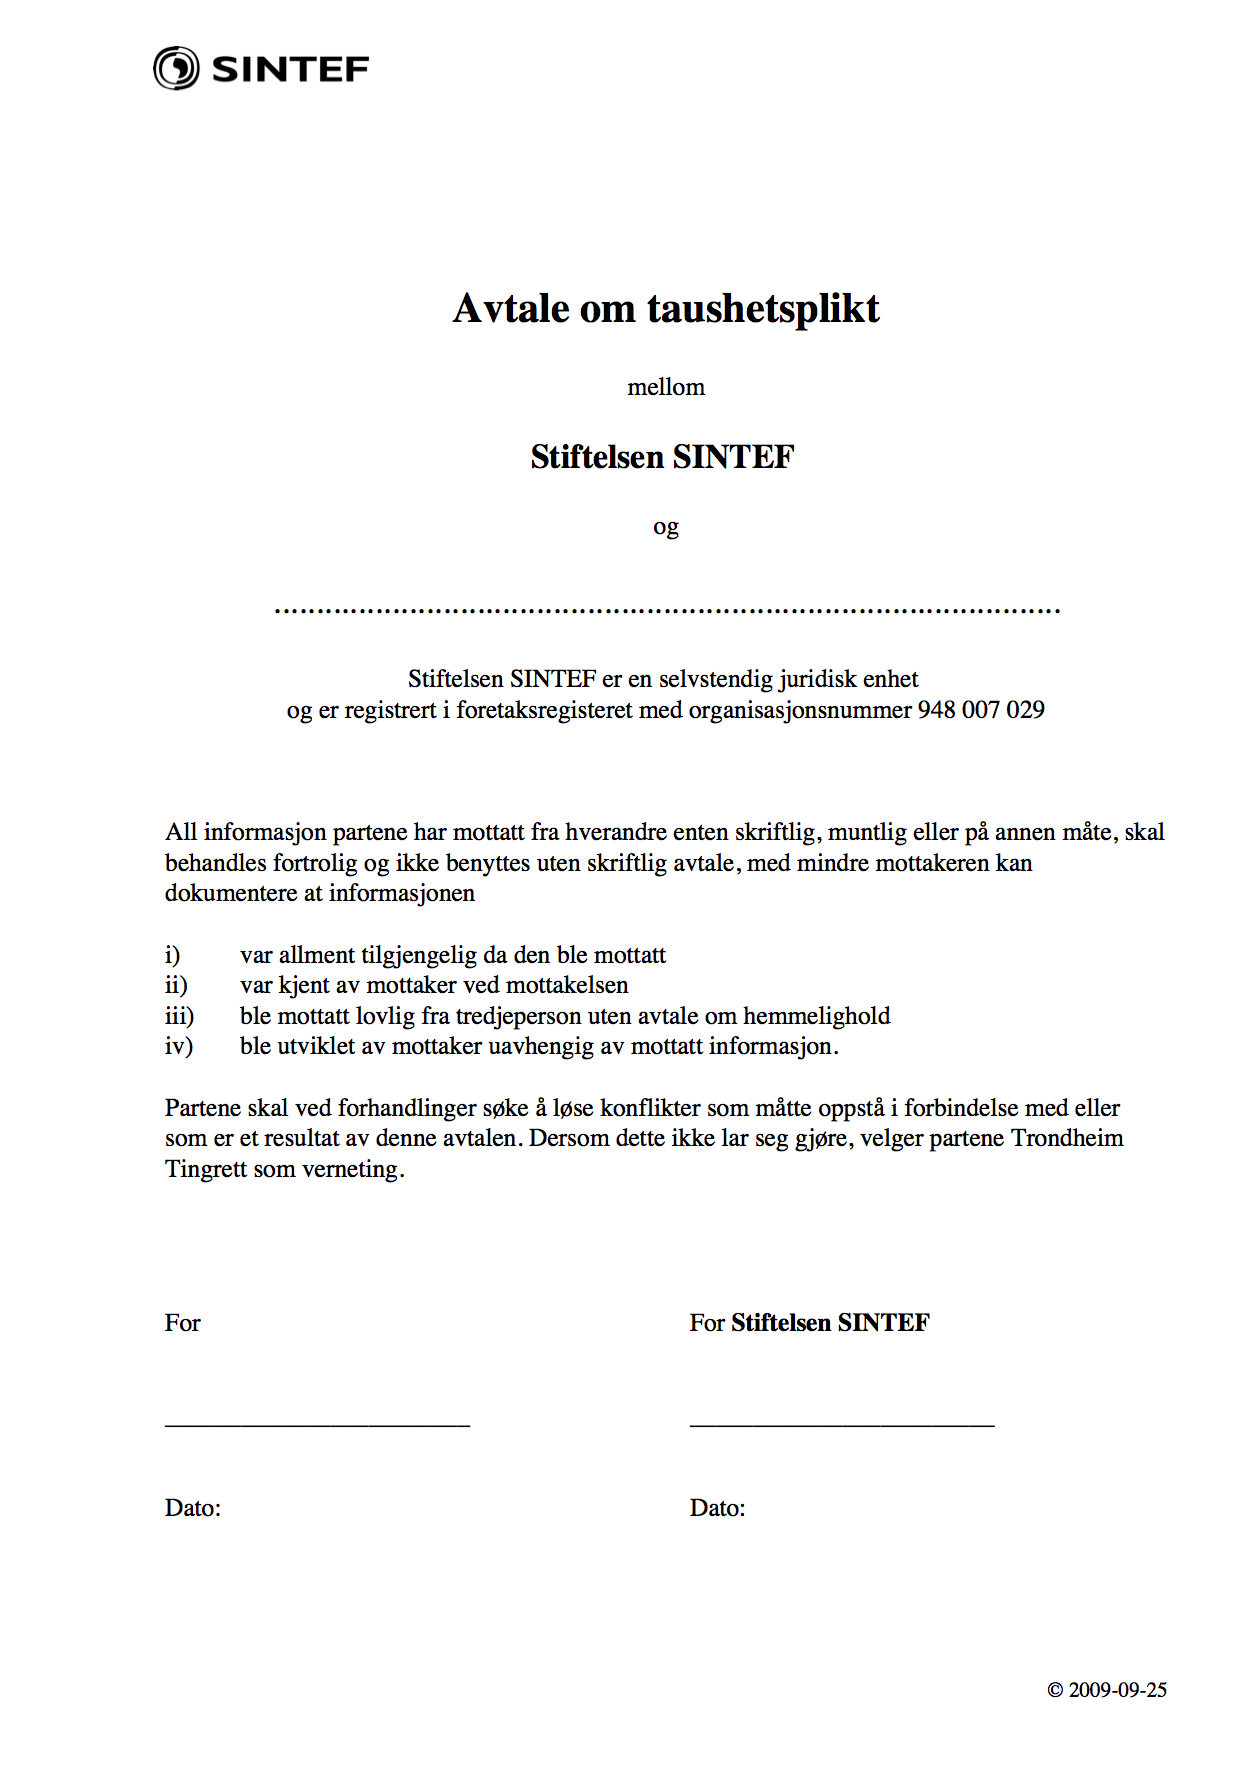
\includegraphics[trim = 0mm 40mm 0mm 0mm, clip, width=\textwidth]{images/taushetsplikt.png}
\end{center}
\end{figure}

\end{document}
